\documentclass[preprint,3p,
a4paper]{elsarticle} %review=doublespace preprint=single 5p=2 column
%%% Begin My package additions %%%%%%%%%%%%%%%%%%%

\usepackage[hyphens]{url}

  \journal{Food Microbiology} % Sets Journal name
\usepackage{amssymb,amsmath}
\usepackage{lineno} % add
  \linenumbers % turns line numbering on

\usepackage{graphicx}
%%%%%%%%%%%%%%%% end my additions to header

\usepackage[T1]{fontenc}
\usepackage{lmodern}
\usepackage{ifxetex,ifluatex}
\usepackage{fixltx2e} % provides \textsubscript
% use upquote if available, for straight quotes in verbatim environments
\IfFileExists{upquote.sty}{\usepackage{upquote}}{}
\ifnum 0\ifxetex 1\fi\ifluatex 1\fi=0 % if pdftex
  \usepackage[utf8]{inputenc}
\else % if luatex or xelatex
  \usepackage{fontspec}
  \ifxetex
    \usepackage{xltxtra,xunicode}
  \fi
  \defaultfontfeatures{Mapping=tex-text,Scale=MatchLowercase}
  \newcommand{\euro}{€}
\fi
% use microtype if available
\IfFileExists{microtype.sty}{\usepackage{microtype}}{}

\ifxetex
  \usepackage[setpagesize=false, % page size defined by xetex
              unicode=false, % unicode breaks when used with xetex
              xetex]{hyperref}
\else
  \usepackage[unicode=true]{hyperref}
\fi
\hypersetup{breaklinks=true,
            bookmarks=true,
            pdfauthor={},
            pdftitle={Plant-based meat alternatives and their associated microbial communities},
            colorlinks=false,
            urlcolor=blue,
            linkcolor=magenta,
            pdfborder={0 0 0}}

\setcounter{secnumdepth}{5}
% Pandoc toggle for numbering sections (defaults to be off)


% tightlist command for lists without linebreak
\providecommand{\tightlist}{%
  \setlength{\itemsep}{0pt}\setlength{\parskip}{0pt}}


% Pandoc citation processing
\newlength{\cslhangindent}
\setlength{\cslhangindent}{1.5em}
\newlength{\csllabelwidth}
\setlength{\csllabelwidth}{3em}
\newlength{\cslentryspacingunit} % times entry-spacing
\setlength{\cslentryspacingunit}{\parskip}
% for Pandoc 2.8 to 2.10.1
\newenvironment{cslreferences}%
  {}%
  {\par}
% For Pandoc 2.11+
\newenvironment{CSLReferences}[2] % #1 hanging-ident, #2 entry spacing
 {% don't indent paragraphs
  \setlength{\parindent}{0pt}
  % turn on hanging indent if param 1 is 1
  \ifodd #1
  \let\oldpar\par
  \def\par{\hangindent=\cslhangindent\oldpar}
  \fi
  % set entry spacing
  \setlength{\parskip}{#2\cslentryspacingunit}
 }%
 {}
\usepackage{calc}
\newcommand{\CSLBlock}[1]{#1\hfill\break}
\newcommand{\CSLLeftMargin}[1]{\parbox[t]{\csllabelwidth}{#1}}
\newcommand{\CSLRightInline}[1]{\parbox[t]{\linewidth - \csllabelwidth}{#1}\break}
\newcommand{\CSLIndent}[1]{\hspace{\cslhangindent}#1}

\usepackage{setspace}
\doublespacing
\usepackage{caption}
\usepackage{xcolor}
\usepackage{booktabs}
\usepackage{longtable}
\usepackage{array}
\usepackage{multirow}
\usepackage{wrapfig}
\usepackage{float}
\usepackage{colortbl}
\usepackage{pdflscape}
\usepackage{tabu}
\usepackage{threeparttable}
\usepackage{threeparttablex}
\usepackage[normalem]{ulem}
\usepackage{upquote}
\usepackage{makecell}
\usepackage{inputenc}
\newcommand{\beginsupplement}{ \setcounter{table}{0} \renewcommand{\thetable}{S\arabic{table}} \setcounter{figure}{0} \renewcommand{\thefigure}{S\arabic{figure}} }
\usepackage{booktabs}
\usepackage{longtable}
\usepackage{array}
\usepackage{multirow}
\usepackage{wrapfig}
\usepackage{float}
\usepackage{colortbl}
\usepackage{pdflscape}
\usepackage{tabu}
\usepackage{threeparttable}
\usepackage{threeparttablex}
\usepackage[normalem]{ulem}
\usepackage{makecell}
\usepackage{xcolor}



\begin{document}


\begin{frontmatter}

  \title{Plant-based meat alternatives and their associated microbial
communities}
    \author[LMM]{Franz-Ferdinand Roch%
  %
  }
  
    \author[LMM]{Monika Dzieciol%
  %
  }
  
    \author[LMM]{Narciso Martin Quijada%
  %
  }
  
    \author[LMM]{Patrick-Julian Mester%
  %
  }
  
    \author[LMM]{Evelyne Selberherr%
  \corref{cor1}%
  }
   \ead{evelyne.selberherr@vetmeduni.ac.at} 
      \affiliation[LMM]{Unit of Food Microbiology, Institute of Food
Safety, Food Technology and Veterinary Public Health, Department for
Farm Animals and Veterinary Public Health, University of Veterinary
Medicine Vienna}
    \cortext[cor1]{Corresponding author}
  
  \begin{abstract}
  Plant based meat alternatives (PBMA) are currently a popular way for
  flexitarians to reduce their meat consumption without having to give
  up the pleasure of burgers and Co.~But so far it is still unclear
  whether these substitutes are a short-lived trend or become
  established in the long term. Over the last few years, the trend of
  increasing sales and diversifying the product range has continued, but
  publication activities in this field are currently limited mainly to
  market research and food technology topics. The paucity of microbial
  investigations of PBMAs has prompted us to examine vegan meat
  substitutes from Austrian supermarkets using culture-dependent and
  culture-independent methods to identify potential product-specific,
  microbial communities. Based on 16S rRNA gene amplicon sequencing the
  majority of the products were dominated by lactic acid bacteria
  (either \emph{Leuconostoc} or \emph{Latilactobacillus}), and generally
  had low alpha diversity. \emph{Proteobacteria}-dominated the other
  part of the products, on which the dominance of single amplicon
  sequence variants (ASVs) is noticeably weaker and the alpha diversity
  distinctly higher than in the lactic acid bacteria (LAB) dominated
  samples. However, the cultivability of the represented genera was
  lower in the \emph{Proteobacteria}-dominated samples, which raises the
  legitimate question of whether living representatives of these genera
  are actually found on the final products. In addition to LABs, a high
  diversity of different \emph{Bacillus}, but also some
  \emph{Enterobacteriaceae} and potentially pathogenic species were
  isolated with the culturing approach. We assume that especially the
  dominance of heterofermentative LABs has a high relevance for the
  product stability and quality and that there is potential to increase
  shelf life of the products. The number of isolated
  \emph{Enterobacteriaceae} and potential pathogens were relatively low,
  but they still demonstrated that these products are certainly suitable
  nursery for them. Even though all the examined products had to be
  heated before consumption, we would like to point out that the lack of
  consumer experience with this type of product is relatively low, which
  is why we believe that further research into product safety, taking
  these aspects into account, would be desirable.
  \end{abstract}
    \begin{keyword}
    meat analogue \sep vegan meat \sep meat substitute \sep microbial
profile \sep food safety \sep 
    plant protein
  \end{keyword}
  
 \end{frontmatter}

\hypertarget{introduction}{%
\section{Introduction:}\label{introduction}}

For most of the population of the Western world, meat consumption is an
integral part of their diet. An average U.S. American consumed 102 kg
and a European Union citizen 69 kg of meat in 2020 {[}1,2{]}. The global
meat consumption increased from 24 kg per year and capita in 1990 to 34
kg in 2020 {[}2,3{]}. Although the OECD estimates that consumption will
level off at around 35 kg per year and capita by 2030, the total meat
consumption will further increase with population growth {[}3{]}. This
globally growing appetite for meat is linked to livestock farming and
consequently plays a major role in the ecological issues we are
currently facing, like land degradation, climate change, water pollution
and loss of biodiversity {[}4,5{]}. Additionally, common industrial
animal husbandry influences public health by supporting the spread of
antibiotic resistances and vector-borne disease {[}5--7{]}. Further,
high meat consumption, as practiced in the Western world and
increasingly in transition countries, contributes significantly to many
widespread common diseases, like coronary heart disease, diabetes
mellitus or colorectal cancer and consequently burdens health care
systems {[}8--11{]}. These mentioned aspects are main drivers for more
and more people in western civilization to change their meat consumption
routines {[}12,13{]}. In a survey, conducted 2021 in ten different
European countries, 2\% of the participants referred to themselves as
vegans, 5\% as vegetarians, 3\% as pescetarians and 30\% as flexitarians
{[}14{]}. The last group is characterized, among other things, by the
fact that they want to reduce their meat consumption, but do not want to
give up the positive experience that comes with it. As main target
group, flexitarians account for about 90\% of the sales of plant based
meat alternatives {[}15{]}. A market research within ``The Smart Protein
Project'' noted a sales value increase of 82\% for plant-based meat
(vegan and vegetarian) within 2018 and 2020 for Austria {[}16{]}. The
sales of this product group and the number of different products have
increased strongly over the last few years {[}16,17{]}. Despite the
increased consumption of these products, there have been only a few
studies on their microbiological properties. However, these would be
important for ensuring food safety, characterizing potential hazards,
assessing risks, and for sustainability questions. Since two of the UN's
sustainability goals (goal 2 -- zero hunger and 12 -- responsible
consumption and production) affects our eating habits, increased
attention should be paid to reducing food waste. As 30\% of food
products in primary processing does not even reach the consumer, mainly
because of microbial spoilage or pathogen contamination, it is essential
to improve the knowledge of the microbial communities of our food, which
could help to increase the shelf life and reduce the contamination with
pathogens. Still largely unanswered is the question if and how a high
microbial diversity on food (consisting of living and dead microbiota)
can have a positive effect on consumer's health. For example, a high
microbial diversity permanently stimulates the innate and adaptive
immune system and provides resistance against colonizing pathogens
{[}18--20{]}. It was also supposed recently, that the loss of microbial
diversity including the disappearance of ancestral indigenous
microbiota, which is currently happening in western countries, affects
human health and contributes to post-modern conditions such as obesity
and asthma {[}21,22{]}. For all these research questions fundamental
knowledge on the microbial compositions on food are necessary, but still
lacking. Since, little is known on these products, we sampled a
selection of plant-based meat alternatives (PBMA) available in Austrian
supermarkets to investigate the general microbial community patterns.
Further, we described characteristic microbial profiles and compared
four groups of the most common product types (pea and soybean based
products with either ``minced'' (minced meat, burgers, etc.) or
``fibrous'' (meat chunks, Schnitzel, etc.) texture. We hypothesized that
products within one group have, based on similar protein processing,
more similar communities than between the groups. Since we examined a
relatively undescribed product group, we have chosen a combined approach
using culture-dependent and culture-independent techniques. This allowed
a more complete description of the microbial community than any of the
applications could stand on their own, but also raised additional
questions and uncertainties that are relevant to future microbial
research of (highly processed) foods.

\hypertarget{material-and-methods}{%
\section{Material and Methods}\label{material-and-methods}}

\hypertarget{sample-acquisition}{%
\subsection{Sample acquisition}\label{sample-acquisition}}

We purchased 32 different PBMA, between July 12 and July 14, 2021, from
four supermarket chains in Vienna, Austria. The focus was on pea- and
soybean- protein based products with either a minced or a fibrous
texture, since they were the most common representatives of PBMA at this
time point in Austria. Additional criteria for the selection were, that
the products where entirely plant-based (vegan) and do not contain
fermented products, like tofu. Beside these characteristics, the samples
were different in their composition, packing, shelf life, etc. (Table
\ref{tab1}). All samples were transported refrigerated and stored at 4°C
until processing. Sample processing took place within the shelf life and
latest five days after purchase.

\hypertarget{sample-preparation}{%
\subsection{Sample preparation}\label{sample-preparation}}

In total, 10 g of each sample, representing all layers of a product,
were placed in sterile Stomacher\textsuperscript{\textregistered}400
classic strainer bags (Seward Ltd, Worthing, United Kingdom) and diluted
with 90 ml sterile phosphate buffered saline (PBS, gibco, Bleiswijk, The
Netherlands). A BagMixer\textsuperscript{\textregistered} 400 CC
(Interscience, Puycapel, France) was used to mechanically comminute the
samples for 120 s. To remove coarse food particles, the homogenates were
centrifuged at 300 rcf (relative centrifugal force) for 2 min at room
temperature (RT) using an Eppendorf Centrifuge 5810R and an A-4-62 rotor
(Eppendorf Corporate, Hamburg, Germany). The remaining supernatants were
transferred to new tubes and centrifuged at 3,000 rcf (30 min at RT).
The obtained cell pellets were diluted 1:10 (v/v) with sterile PBS and
were used freshly for bacterial and fungal isolation, or were frozen at
-80°C for later DNA extraction.

\hypertarget{bacterial-and-fungal-isolation}{%
\subsection{Bacterial and fungal
isolation}\label{bacterial-and-fungal-isolation}}

We carried out two sets of cultivation experiments. The first set was
done with a general selection of media (Columbia agar (BioMérieux, Marcy
l'Etoile, France), Violet Red Bile Glucose agar (VRBG, Biokar
diagnostics, Allonne, France), brain heart infusion agar (BHI broth
(Biokar diagnostics) + 1.5\% agar (bacteriological agar type E, Biokar
diagnostics)), plate count agar (PCA, Biokar diagnostics), Rose Bengal
Chloramphenicol agar (Biokar diagnostics), and Baird Parker agar
(GranuCult\texttrademark, Merck, Darmstadt, Germany)), to get a broad
range of the expected microbial community. The plates were inoculated
with 100 \(\mu\)l of a 10\textsuperscript{2} dilution and aerobically
and semi-anaerobically (using GENbox anaer, BioMérieux, in BD
BBL\texttrademark GasPak\texttrademark systems, Becton Dickinson, New
Jersey, United States) incubated at 37°C. In order to recover high
amounts of different species, the plates were incubated for 16-68 hr,
depending on colony size and growth density. Samples with growth
densities too high for picking single colonies after 16 hr of incubation
were diluted 10\textsuperscript{3} or 10\textsuperscript{4} in sterile
PBS and plated again. For the second media set we used the information
from the 16S rRNA gene amplicon sequencing to select specific media and
growth conditions in order to isolate representatives of genera we could
not isolate under the first culturing conditions. Depending on the
sample specific microbial composition we used Luria Bertani Agar (1\%
tryptone (Oxoid, Basingstoke, UK), 0.5\% yeast extract
(micro-granulated, Roth, Karlsruhe, Germany), 1\% NaCl (Sigma-Aldrich,
St.~Louis, USA), 2\% agar, pH 7.0), nutrient agar (0.5\% casein peptone,
tryptic digest (Roth), 0.3\% beef extract powder (Fluka analytical,
Seelze, Germany), 1.5\% agar, pH 7.0), trypto-casein soy agar
(TSA,Biokar diagnostics), marine agar (marine broth (Roth) + 1.5\% agar
), corynebacterium agar (1\% casein peptone, tryptic digest, 0.5\% yeast
extract, 0.5\% D(+)-glucose (Roth), 0.5\% NaCl, 1.5\% agar, pH 7.3),
De-Man-Rogosa-Sharpe agar (MRS, Oxoid) and pseudomonas agar F (1\%
tryptone, 1\% casein peptone, 0.15\%
K\textsubscript{2}HPO\textsubscript{4}, 0.15\% (Roth),
MgSO\textsubscript{4} (Merck), 1\% glycerol (Roth), 1.5\% agar) and
cultivated the samples (dilution
10\textsuperscript{2}-10\textsuperscript{5}) aerobically at 25°C for 48
hr. In both cultivation experiments, we selected morphologically unique,
single colonies for re-cultivation followed by 16S rRNA gene Sanger
sequencing of the pure cultures for identification. DNA was extracted,
using a protocol modified after Walsh et al. {[}23{]}, by lysing pure
cultures with 100 \(\mu\)l 0.01 M TRIS/HCl
(Trizma\textsuperscript{\textregistered}base, Sigma-Aldrich, St.~Louis,
United States) and 400 \(\mu\)l 2.5\%
Chelex\textsuperscript{\textregistered}100 resin solution (BioRad,
Hercules, United States) at 95°C for 10 min, followed by centrifugation
with 15,000 rcf for 30 s. The supernatants were subsequently used for
16S rRNA gene PCR, using a final concentration of 200 nM of each of the
universal primers from LGC Genomics GmbH (Berlin, Germany; 27F -- 5'-GAG
TTT GAT C\textbf{M}T GGC TCA G-3' and 1492R -- 5'-GG\textbf{Y} TAC CTT
GTT ACG ACT T-3'), 0.025 U/\(\mu\)l Platinum\texttrademark Taq
DNA-Polymerase (Invitrogen\texttrademark, Vilnius, Lithuania), 1x TaqMan
PCR buffer, 2 mM MgCl\textsubscript{2}, and 250 nM dNTP Mix (Thermo
Scientific\texttrademark, Vilnius, Lithuania). For the PCR a protocol of
95°C for 5 min (Taq activation) followed by 35 cycles of 40 s at 95°C
(denaturation) 40 s at 52°C (annealing ) and 1 min at 72°C (elongation)
was used. For negative control a reaction with ddH\textsubscript{2}0 as
well as a reaction the negative extraction control were performed.
In-house \emph{Listeria monocytogenes} DNA served as positive control.
All PCR products were checked with a QIAxcel DNA High Resolution Kit
(Qiagen, Hilden, Germany) in a QIAxcel Advanced system (Qiagen). Samples
without detectable amounts of PCR products were used for an ITS2 gene
PCR (200 nM of each of the primers ITS3 -- 5'-GCA TCG ATG AAG AAC GCA
GC-3' and ITS4 -- 5'-TCC TCC GCT TAT TGA TAT GC-3' (White et al.~1990),
0.025 U/\(\mu\)l Platinum\texttrademark Taq DNA-Polymerase
(Invitrogen\texttrademark), 1x TaqMan PCR buffer, 2 mM
MgCl\textsubscript{2}, and 250 nM dNTP Mix (Thermo
Scientific\texttrademark), with a protocol of 95°C for 5 min (Taq
activation) followed by 30 cycles of 40 s at 94°C, 40 s at 56°C and 1
min at 72°C). For cultures, negative in 16S rRNA and ITS2 PCR, we
repeated the extraction with the NucleoSpin tissue kit (Machery-Nagel,
Düren, Germany), using the manual in combination with the
recommendations for hard-to-lyse bacteria. LGC Genomics GmbH purified
and sequenced the PCR products in one direction (using 27F primer for
16S rRNA and ITS4 for the ITS2 region). Potential pathogens and
unclassified \emph{Enterobactericeae} were further whole genome
sequenced with FLO-MIN106 flow cells on a MinION Mk1C (Oxford Nanopore
Technologies, Oxford, UK). The library preparation for this approach was
done according to the protocol of Oxford Nanopore Technologies
(``Ligation sequencing gDNA - native barcoding (SQK-LSK109 with
EXP-NBD196)'' {[}24{]}) using the
NEBNext\textsuperscript{\textregistered} FFPE DNA repair kit (New
England BioLabs\textsuperscript{\textregistered} Inc., Ipswich, United
States) for DNA repair and end-preparation, NEB Blunt/TA Ligase Master
Mix (New England BioLabs\textsuperscript{\textregistered} Inc.) and
Native Barcoding Kit 96 (EXP-NBD196, Oxford Nanopore Technologies), for
native barcode ligation, Adapter Mix II (Oxford Nanopore Technologies)
and NEBNext\textsuperscript{\textregistered} Quick Ligation Module (New
England BioLabs\textsuperscript{\textregistered} Inc.), for adapter
ligation, Agencourt AMPure XP beads (Beckman Coulter\texttrademark), for
clean-up steps and SQK-LSK109 sequencing kit (Oxford Nanopore
Technologies).

\hypertarget{s-rrna-gene-amplicon-sequencing}{%
\subsection{16S rRNA gene Amplicon
sequencing}\label{s-rrna-gene-amplicon-sequencing}}

For direct DNA extraction the DNeasy\textsuperscript{\textregistered}
PowerFood\textsuperscript{\textregistered} Microbial Kit (Qiagen) was
used. That for, the in PBS stored cell pellets (-80°C) were thawed,
centrifuged (3,000 g, 30 min) and resuspended in 450 \(\mu\)l MBL
buffer. Deviating from the DNeasy\textsuperscript{\textregistered}
PowerFood\textsuperscript{\textregistered} Microbial Kit Handbook
{[}25{]}, the lysis step was proceeded in Lysing Matrix A, 2 ml tubes
(MP Biomedicals Germany GmbH, Eschwege, Germany). 16S rRNA gene amplicon
library generation and sequencing was performed at the Vienna Biocenter
Core Facilities NGS Unit (Vienna, Austria, www.vbcf.ac.at). Sequencing
libraries of the 16S rRNA gene (V3/4 region) were prepared based on
Illumina 16S Metagenomic Sequencing Library Preparation recommendations.
Primers 341F (5'-CCT ACG GG\textbf{N} GGC \textbf{W}GC AG-3') and 805R
(5'-GAC TAC \textbf{HV}G GGT ATC TAA TCC-3') (Klindworth et al.~2013)
were used together with Illumina adapter sequences (5'-CGT CGG CAG CGT
CAG ATG TGT ATA AGA GAC AG-3' and 5'-GTC TCG TGG GCT CGG AGA TGT GTA TAA
GAG ACA G-3', respectively) for amplification. Libraries were
constructed by ligating sequencing adapters and indices onto purified
PCR products using the Nextera XT Sample Preparation Kit (Illumina).
Equimolar amounts of each of the purified amplicons were pooled and
sequenced on an Illumina MiSeq Sequencer with a 300 bp paired-end read
protocol.

\hypertarget{sequence-processing-and-statistics}{%
\subsection{Sequence Processing and
Statistics}\label{sequence-processing-and-statistics}}

The data obtained from the MiSeq sequencing went through a QIIME
2\texttrademark v2021.4.0 {[}26{]} workflow including the integraded
demultiplexing, DADA2 denoising and quality control filtering. The
taxonomic classification was done with the Scikit-learn algorithm using
a pre-trained full-length-uniform-classifier based on the SILVA 138.1
database {[}27--31{]}. After removal of sequences with mitochondrial or
chloroplastic origin, further analyses were performed with R {[}32{]}.
To estimate the alpha diversities of the samples Hill-Simpson and
Hill-Shannon diversity were calculated using the ``iNEXT'' package
{[}33{]}, based on 99.5\% coverage rarefied samples {[}34,35{]}. Group
comparisons were done with Kruskal-Wallis tests followed by
Bonferroni-alpha-corrected Dunn's tests for pairwise comparisons. For
beta diversity analyses the samples were rarefied with 100 iterations
depending on a coverage of 99.5\% using the package ``phyloseq''
{[}36{]} and ``metagMisc'' {[}37{]}. Based on that we generated distance
matrices with Bray-Curtis dissimilarities, Jaccard indices and
Jensen-Shannon divergence (JSD) and use them for graphical
(t-distributed stochastic neighbor embedding - tSNE) and statistical
(PERMANOVA, LEfse) analysis. For tSNE we used the ``Rtsne'' package
{[}38{]} with a maximum of 999 iterations, a perplexity of 5 and two
initial dimensions, as recommended by Oskolkov {[}39{]}. The high
variability of the products and little knowledge on the underlying
production conditions made it impossible to find adequate variables for
PERMANOVA, besides the main protein source and the texture. The
producing facility as additional variable would be meaningful, but the
product assortment is dominated by one company, which made the model
design very unbalanced. PERMANOVA was done with the ``vegan'' package
{[}40{]} using ``betadisp'' to check for homogeneous dispersion and
``adonis'' functions for PERMANOVA with 999 iterations using main
protein source and texture as explanation variables. LEfse was done with
the relative abundance data of the coverage rarefied data in combination
with ``phyloseqCompanion'' package {[}41{]}, for data transformation and
the LEfse Bioconda tool by Segata et al. {[}42{]}, using the protein
source and texture as class, a normalization of 10\textsuperscript{6}
and a log\textsubscript{10} LDA score threshold of 4.0. In parallel, a
group comparison for the same features, as examined with LEfse, was done
with Kruskal-Wallis tests followed by a Benjamin-Hochberg alpha
correction.\newline  The Sanger sequences from the isolates were trimmed
using the ``SangerRead'' function within the ``sangeranalyseR'' package
{[}43{]} with a Phred score mean quality cutoff of 40 and a sliding
window size of 15 bp. Trimmed sequences, with \textgreater100 bp length,
were classified with the ``assignTaxonomy'' function of the ``dada2''
package {[}44{]} in R (with kmer size 8 and 50 bootstrap replicates),
based on an RDP (Ribosomal Database Project) Naïve Bayesian Classifier
algorithm (Wang et al.~2007). Further, the isolate sequences were
assigned to a database generated from the MiSeq data set to connect the
culture-based and culture-independent approaches. For figure \ref{fig1},
the isolate sequences of each genus were clustered within each sample,
group and producer using the ``IdClusters'' function from the
``DECIPHER'' package {[}45{]} with a cutoff of 0.06. More clusters
within each genus were interpreted as a higher species or strain
diversity within each genus.\newline The whole genome data sequenced
with the MinION were trimmed and filtered with Filtlong v0.2.1 {[}46{]},
assembled with Flye v2.9 {[}47,48{]} followed by several polishing steps
(four repetitions of Racon v1.5.0 {[}49{]} and a final step with Medaka
v1.6.0 {[}50{]} ), before they were used in the TORMES v1.3.0 {[}51{]}
workflow. Within the TORMES workflow genomes were assembled with SPAdes
v3.15.2 {[}52{]}, gene prediction and annotation was done with Prodigal
v2.6.3 {[}53{]} and Prokka v1.14.6 {[}54{]}. Abricate v1.0.1 {[}55{]}
with the comprehensive antibiotic resistance database (CARD) {[}56{]}
and the virulence factor database (VFBD) {[}57{]} for antibiotic
resistance and virulence factor screening. The assembled genomes were
classified with the GTDB-Tk v2.2.0+ {[}58,59{]} and rLMST {[}60{]}.
BTyper3 {[}61{]} was used for isolates classified with GTDB-Tk as
\emph{Bacillus\_A paranthracis}. Lactic acid bacteria with good quality
genomes were additionally examined with BlastKOALA v2.3 {[}62{]} and
antiSMASH v6.1.1 {[}63{]}. The genes within clusters predicted with
antiSMASH where then blasted using BLASTP. All tools were used with
default settings if not mentioned otherwise.

\hypertarget{results}{%
\section{Results}\label{results}}

\hypertarget{product-descriptions}{%
\subsection{Product descriptions}\label{product-descriptions}}

The four groups did not have the same sizes, since the product variety
in the selected supermarkets was not large enough in the time period of
sampling to get enough representatives for each group. Still, we had an
overall of 16 pea-based and 16 soybean-based products (Table 1). Beside
the four main properties, the products were quite diverse. Particularly
noteworthy is the number of ingredients used per product (4-27, with a
total of about 120 different used ingredients within the 32 sampled
products) and the large range of shelf life. The products are also
different on factors, which might influence the bacterial composition,
i.e.~pre-heating or freezing steps, as well as packing in modified
atmosphere. Most of the products had clear cooking instructions on the
labels, including the recommendation for thorough cooking (Table
\ref{tab1}). In total, 27 samples were packed in modified atmosphere
with unknown composition. Out of 30 samples sold refrigerated (the other
two frozen). According to the label six products were frozen at any
point during the retail chain (Table \ref{tab1}).

\hypertarget{cultivable-microbial-communities}{%
\subsection{Cultivable microbial
communities}\label{cultivable-microbial-communities}}

In total, 470 colonies were picked and selected for 16S rRNA or ITS2
gene sequencing. Among these, 431 could be classified as bacteria to the
genus level, representing 38 genera in four different phyla (Figure
\ref{fig1}). The remaining isolates could only be assigned to family
level (n=16, all \emph{Enterobacteriaceae}), were fungi (n=20;
\emph{Wickerhamomyces} (n=7), \emph{Pichia} (n=6), \emph{Yarrowia}
(n=3), \emph{Kurtzmaniella} (n=3), \emph{Geotrichum} (n=1)), or stayed
unassigned (n=3). We isolated \emph{Bacillus} from 19,
\emph{Leuconostoc} from 18, \emph{Enterococcus} from 12, and
\emph{Latilactobacillus} from 10 samples. Species from the genus
\emph{Bacillus}, \emph{Leuconostoc} and \emph{Latilactobacillus} could
be isolated from each of the four sample groups.
\emph{Enterobacteriaceae}, which are usually surveyed as an additional
hygiene criterion, were only found in the pea protein products of a
single manufacturer (Figure \ref{fig1}). A selection of these
\emph{Enterobacteriaceae}, of the dominant lactic acid bacteria and
isolates classified by the RDP Naïve Bayesian Classifier algorithm as
potential pathogens (i.e.~\emph{Staphylococcus aureus}, \emph{Bacillus
cereus} group, \emph{Klebsiella} sp.) were whole genome sequenced with a
MinION Mk1c device (Table \ref{tab2}). Most of the sequenced
Enterobacteriaceae were described as established human pathogens
according to Bartlett et al. {[}64{]} (Figure \ref{fig1}). Among these
\emph{Escherichia (E.) coli} is the only food associated pathogen.
Within the genome of the isolated \emph{E. coli} strain several
virulence factors and antimicrobial resistance genes could be annotated
with VFDB and CARD. For example, virulence factors like fimH (Type 1
fimbriae, 97.59\% identity with \emph{E. coli} CFT073) and fyuA (ferric
yersiniabactin uptake, 99.80\% identity with \emph{Yersinia pestis}
CO92), which are associated with Adherent-Invasive E. coli (AIEC)
{[}65{]} and genes asociated with antibiotic resistances like mdfA
(98.38\% identity with accession JQ394987:0-1233) or ampH (98.88\%
identity with accession AP012030.1:396711-395553). The three
\emph{Klebsiella} isolates belonged to the \emph{K. oxytoca} species
complex (KoSC). Two of them were classified by rMLST and the
GTDB-Toolkit as \emph{K. oxytoca} and \emph{K. grimontii}, respectively.
This is consistent with the identified beta-lactamase genes
(\emph{bla}\textsubscript{OXY}), which can be used for species typing in
\emph{Klebsiella} {[}66{]}. \emph{Bla}\textsubscript{OXY-2} was detected
in the \emph{K.oxytoca} and \emph{bla}\textsubscript{OXY-6} in the
\emph{K. grimontii} genome. The third isolate is according to rMLST a
\emph{K. pasteurii} isolate, which is supported by the detection of a
\emph{bla}\textsubscript{OXY-4} gene. Since \emph{K. pasteurii} was not
present in the GTDB at the time of classification, the isolate was
classified as \emph{K. grimontii} (95.91\% ANI to the closest reference
genome). Extended spectrum beta-lactamase (ESBL)- and
Carbapenemase-producing isolates of this species complex are associated
with nosocomial infections {[}66{]}, however, in the isolates of this
study no resistance genes additional to \emph{bla}\textsubscript{OXY}
were detected. The other isolated and whole genome sequenced
\emph{Enterobacteriaceae} isolates were classified as \emph{Citrobacter
braakii}, \emph{Leclercia adecarboxylata} and \emph{Lelliottia amnigena
A}. Within the \emph{Bacillus} genus, the 13 sequenced isolates were
classified as \emph{Bacillus (B.) licheniformis} (n=4), \emph{B.
pumilus} (n=3), \emph{B. paralicheniformis} (n=1), \emph{B. subtilis}
(n=1), \emph{B. velezensis} (n=1) and \emph{Bacillus\_A paranthracis}
(n=3). Since \emph{B. paranthracis} can cause foodborne illnesses
{[}67{]}, their genomes were additionally analyzed with BTyper3
(Supplements table \ref{tabSM2}), which predicted the presence of the
relevant non-hemolytic enterotoxin (nhe) complex, which is associated
with diarrhea, and other virulence factors. The \emph{Staphyloccous
aureus} isolate genome contained no relevant genes for antimicrobial
resistances or staphylococcal enterotoxins, but several other virulence
genes (Supplements table \ref{tabSM2}). The analysis of the lactic acid
bacteria was focused on spoilage potential (enzymatic repertoire for
metabolite production) and preservative aspects. The sequenced
\emph{Leuconostoc} and \emph{Latilactobacillus} isolates possessed genes
to produce metabolites associated with food spoilage, like
butane-2,3-dione (diacetyl), 3-hydroxybutan-2-one (acetoin),
2-hydroxypropanoate (lactate), acetate and ethanol. One of the \emph{Ln.
mesenteroides} isolates we were able to detect the genes for leucocin
A/sakacin P family class II bacteriocin and the associated relevant
transport proteins, while in \emph{L. sakei} isolates only the
transporter genes were detectable (antiSMASH hits and belonging blastp
best hits in Supplements table \ref{tabSM2}).

\hypertarget{lactic-acid-bacteria-and-gammaproteobacteria-dominate-the-16s-rrna-gene-amplicon-sequences}{%
\subsection{Lactic acid bacteria and Gammaproteobacteria dominate the
16S rRNA gene amplicon
sequences}\label{lactic-acid-bacteria-and-gammaproteobacteria-dominate-the-16s-rrna-gene-amplicon-sequences}}

In total, 28 samples (883,866 sequences; median frequency per sample:
25,627; range: 439-253,681) passed the quality criteria and were
processed with QIIME 2. During the process another sample was removed
due to the low number of remaining reads (n=439) after quality
filtering. Over all samples, the ASVs were assigned to 25 different
Phyla, however, there were only three Phyla with \textgreater3\%
relative abundance in at least one of the samples detected
(i.e.~\emph{Firmicutes} 0.00-94.74\%, \emph{Proteobacteria}
0.00-30.85\%, \emph{Bacteroidota} 0.00-10.84\%). In total, 18 samples
were dominated (\textgreater50\% relative abundance) by
\emph{Firmicutes} (10 samples with \textgreater90\%), while in the other
9 samples \emph{Proteobacteria} were the most abundant. The most common
genera were \emph{Leuconostoc} (detected in 25 samples; 0.03-100.00\%),
\emph{Latilactobacillus} (detected in 21 samples; 0.02-86.38\%),
\emph{Pseudomonas} (detected in 20 samples; 0.36-35.25\%),
\emph{Serratia} (detected in 19 samples; 0.03-8.92\%), and Acinetobacter
(detected in 17 samples; 0.09-15.40\%). The genus \emph{Leuconostoc} was
the most abundant in 13 samples, followed by \emph{Latilactobacillus} (4
products), and \emph{Shewanella} (4 products) (Figure \ref{fig2}). Some
genera were found proportionally high (\textgreater10\%) in one or more
samples, but could not be isolated (i.e.~\emph{Shewanella},
\emph{Xanthomonas}, \emph{Photobacterium}, \emph{Myroides},
\emph{Pediococcus}).

In the tSNE plot we see three distinct clusters (Figure \ref{fig3}),
which we described, based on the dominating genera as
\emph{Leuconostocaceae}-, \emph{Latilactobacillus}- and
\emph{Proteobacteria}-profiles. The clustering is traceable, when
comparing the similarity of the relative abundance patterns of the
samples within each cluster. Although there is some clustering, there is
no clear separation based on the examined variables (main protein
source, status, manufacturer).

\hypertarget{protein-source-and-texture-are-not-the-main-driver-for-the-community-pattern}{%
\subsection{Protein source and texture are not the main driver for the
community
pattern}\label{protein-source-and-texture-are-not-the-main-driver-for-the-community-pattern}}

The Kruskal-Wallis test comparing the Hill-Shannon index between the
four groups (based on proteins source and texture) was significant
(p.value = 0.02), while there was no significant difference comparing
the group-wise Hill-Simpson index (0.05). Post-hoc Dunn's testing with
Bonferroni alpha adjustment showed that when comparing group-wise
Hill-Shannon index only the groups ``pea-fibrous'' and ``pea-minced''
differed significantly (p.value= 0.02 - Supplement Figure
\ref{figSM1}).\newline  The group dispersions were homogenous in all
examined distance methods (i.e.~Bray-Curtis, Jaccard, JSD). The
PERMANOVA showed that texture and protein source significantly affects
the microbial composition (Supplement Table \ref{tabSM1}), but explained
only between 15.94\% and 23.44\% of the total variance. The variance
explanation by the PERMANOVA would increase, if the manufacturer as
variable was added to the model, but since the sampling was very
unbalanced on that, therefore it was renounced.\newline LEfSe identified
several features with an log10 LDA score \textgreater4.0. For
``pea-fibrous'' products those were the genera \emph{Leuconostoc} and
\emph{Enterococcus} and with the corresponding superordinate phylogeny
levels. For ``pea-minced'' products it was mainly the genus
\emph{Pseudomonas}. In ``soy-fibrous'' products two low abundant orders
(i.e.~\emph{Sphingomonadales} and \emph{Burkholderiales}) had a log10
LDA score \textgreater4.0. The orders \emph{Enterobacterales} and
\emph{Flavobacteriales} (Phylum \emph{Bacteroidota}) were identified
(Supplement figure \ref{figSM4}).

\hypertarget{discussion}{%
\section{Discussion}\label{discussion}}

Highly processed food, like the plant-based meat alternatives we
examined in this study, brings challenges to microbiologists. The broad
range of ingredients (\textasciitilde120 in the 32 examined products),
different processing steps, and a variety of equipment lead to many
potential sources for bacterial contamination. The product specific
production processes were not available, but up to the present low
(LMEC) and high moisture extrusion cooking (HMEC) are the most common
commercially used technologies to produce meat textured plant proteins
{[}68{]}. Both methods are based on an interaction of heat, shear force
and pressure, but the conditions for extrusion process depends on the
original protein source and the desired final protein structure
{[}69--71{]} . From the perspective of microbial survival during this
process temperature, pressure and time are the most relevant variables.
These parameters depend strongly on the process settings and can
therefore only serve as a guide. The extruder barrels show temperature
gradients with temperatures at 150-170°C in the high-temperature melting
zone for HMEC {[}72{]}, but the extruder die is approximately 15-25°C
cooler than that {[}73{]}. The barrel temperature for LMEC is general
lower with 120-150°C {[}74{]}. The pressures in this barrels is between
1-4 MPa in HMEC and up to 13 MPa in LMEC {[}74--76{]}. Yu et al.~showed
in different LMEC settings fastest particle residence times (first signs
of the tracer) from 10-40 s and extrudate collection times (complete
tracer passed) from 60 to 120 s, resulting in mean residence times of
35-87 seconds, depending on feed moisture, screw speed and die diameter
{[}77{]}. So far it is described, that vegetative forms of bacteria get
inactivated effectively by this process and only spores of bacteria like
\emph{Bacilli} and \emph{Clostridia} would survive the extrusion process
{[}78,79{]}. However, reactivation of spores during further processing
is possible {[}80{]}. This could be one explanation why \emph{Bacillus}
was isolated from most of the samples (19/32), while the relative
abundance of 16S rRNA gene DNA is relatively low, compared to other
genera. We assume, due to this initial extrusion procedure, the main
protein is not the source for most of the living bacterial cells we have
isolated from the products. Highly probable contamination sources are
the addition of ingredients, especially spices and herbs {[}81{]}, and
the production environment.

Based on the microbial distribution patterns from the MiSeq data, we
roughly describe three different community profiles. Lactic acid
bacteria dominated two of them (14/28 \emph{Leuconostocaceae} dominated
samples, 4/28 \emph{Latilactobacillus} dominated samples). The majority
of these samples, was dominated by one ASV, which are mostly assignable
to the isolates taken, which suggests that these species are actually
active in the final product. Based on whole genome sequencing of
representative isolates the ASVs and isolates could be classified as
\emph{Leuconostoc} (\emph{Ln.}) \emph{mesenteroides} and
\emph{Latilactobacillus} (\emph{L.}) \emph{sakei}. \emph{Ln.
mesenteroides} and the also isolated \emph{Ln. citreum} belong among
others to the most isolated lactic acid bacteria from plants and
plant-based food {[}82{]}. \emph{Ln. mesenteroides} subsp. are important
fermenters for products like kimchi and sauerkraut {[}83{]}, or soybean
paste {[}84{]}. Other positive features of \emph{Ln. mesenteroides} are
potential probiotic properties of some strains and antimicrobial
activities against pathogenic bacteria, like \emph{Salmonella
typhymurium} and \emph{Listeria monocytogenes} {[}85,86{]}.
Nevertheless, \emph{Ln. mesenteroides} is usually described as common
spoiler for meat, meat products and other food, asssociated with
off-odors, off-flavours, slime and gas production {[}89{]}, especially
in combination with modified atmosphere packaging and cold storage
{[}90--92{]}. Since the sequenced isolates possessed genes for enzymes
producing metabolites associated with spoilage (diacetyl, acetoin,
lactate, acetate, ethanol) and were clearly dominating most of the
products, we assume, that \emph{Ln. mesenteroides} is a very common
spoiler in these product group. Targeting this species, might help to
prolong the shelf life of PBMAs. Similar properties were attributed to
\emph{L. sakei}. It was described as fermenters particularly for
sausages {[}93{]}, and vegetable products {[}94{]}, as producer of
bacteriocines {[}95{]}, and as probiotics {[}96{]}. However, the
\emph{L. sakei} isolates examined also had the genetic potential to
produce the same spoilage associated metabolites as the
\emph{Leuconostoc} isolates.

Geeraerts et al., 2020 examined ready to vegetarian, vegan and insect
based meat alternative, including products with fermented ingredients,
like fermented sour dough. Based on that, they assumed sour dough as
main source for \emph{L. sakei}, which they isolated most {[}97{]}.
Different to that study, we excluded products with fermented
ingredients, but vinegar. Still we found large amounts of lactic acid
bacteria in the examined products. Unlike Geeraerts et al., the majority
of the samples in ours study were dominated by \emph{Leuconostoc}, but
we could not determine this by product characteristics. For kimchi and
other plant products is described, that \emph{Leuconostoc},
\emph{Entercoccus} and \emph{Lactococcus}, as generalists act as initial
colonizers, followed later by \emph{Lactobacillus}, \emph{Pediococcus}
and \emph{Weissella} {[}82{]}. This can be explained by a better
adaptability to environmental conditions (e.g.~through a large number of
accessory genes), but also by the already high population density on the
ingredients, while in later stages decreasing pH values inhibits
\emph{Leuconostoc} species sensitive to acids {[}82{]}. However, the
examined products were very diverse in their shelf life, so it was
impossible to conclude, whether \emph{Latilactobacillus} dominated
samples, were in a later stage of shelf life than the \emph{Leuconostoc}
dominated samples. In vegan meat alternatives, the drop in pH should not
be comparable to kimchi (pH 4.0) {[}98{]}. It ranks in the range of
5.4-6.6 {[}97,99{]}, and thus should not favour \emph{L. sakei}. In
general, in both species there are strains that are able to grew at 4°C
{[}90,94,100{]}, although \emph{Ln. mesenteroides} strains, examined by
Comi and Iacumin grew faster at 4°C than \emph{L. sakei} {[}101{]}.
\emph{Leuconostoc} spp., among these \emph{Ln. mesenteroides} and
\emph{Ln. citreum} are described to inhibit the growth of \emph{L.
sakei} strains {[}102{]}, but it was also demonstrated, that \emph{L.
sakei} is able to inhibit the growth of \emph{Ln. mesenteroides}, when
the are inoculated equally to cooked bacon {[}103{]}. \emph{L.sakei} is
highly adapted to protein rich meat and fish environments and so has
reduced abilities for amino acid biosynthesis {[}104{]}. The \emph{L.
sakei} isolates from this study lack amino acid biosynthesis pathways
for Threonine, Cysteine, Methionine, Valin, Isoleucin, Leucin, Arginin
and Tryptophane. However, these pathways were present in the \emph{Ln.
mesenteroides} isolates. Since most of these amino acids has lower
concentrations in plant proteins compared to muscle proteins {[}105{]},
\emph{Ln. mesenteroides} might have some advantages in PBMAs.

Overall, we examined nine samples with high relative abundances of
\emph{Proteobacteria}, mainly \emph{Pseudomonas}, \emph{Psychrobacter}
and \emph{Shewanella}. These three genera are common spoilers in meat
and fish products, especially in products with slightly higher pH
values, like fish, sea food and poultry {[}107{]}. Plant-based meat
products are usually also slightly higher in pH {[}99{]}. Although the
number of ASVs within a these genera is much higher, compared e.g.~with
\emph{Leuconostoc} from other samples, what we associate with different
sources of contamination, there are still single ASVs with relatively
high abundances, which indicates either a large entry from one source or
an active growth on the product at some time point during the
production. The most obvious sources would be the main protein, the used
water (via biofilms in water reservoirs or water hoses) or biofilms
during the process. From the found genera in the MiSeq data, at least 13
are described as biofilm builders in food processing environments
{[}108{]}, among these \emph{Pseudomonas}, \emph{Psychrobacter} and
\emph{Shewanella}. The possibility of biofilm formation on the
processing equipment is high, since many of the used machines are hard
to clean. However, this is contradicted by the fact that among the nine
\emph{Proteobacteria}-dominated samples seven had a very similar
pattern, but were from six different producers. There are no available
studies on the microbial communities of raw soybean or pea proteins, but
16S rRNA patterns of peas or the phyllosphere of soy do not support the
thesis, that this kind of contamination is associated with the main
protein source. Only sample B4, which is the only sample, that is
dominated by \emph{Alphaproteobacteria}, had high similarities to the
microbial community of the soy phyllosphere {[}109{]}. However, some of
the producer just have a few products in this food segment, so we would
not exclude, that they buy already extruded proteins from a large
distributor and use it for their products. Although we assume that most
\emph{Proteobacteria} detected here are dead in the final product, the
collected microbial communities of these products are not irrelevant. On
the one hand, it is possible that bacteria, which are metabolically
active at some point during the process, contributes to the development
of (off-)odors and (off-)tastes, and on the other hand, it can provide
information on whether there are contamination inputs in the ingredients
or process areas that could be considered in the HACCP concept in the
longer term (e.g.~preventing biofilm formations).

Beside the dominating, spoilage associated genera, we also isolated some
\emph{Enterobactericeae}, of which selected isolates where whole genome
sequenced and taxonomically assigned to \emph{Leclercia},
\emph{Atlantibacter}, \emph{Citrobacter}, \emph{Escherichia} and
\emph{Klebsiella}. This confirms the findings of Luchansky et al., who
inoculated beef and vegan burgers with Shiga toxin-producing human
pathogens (i.e.~\emph{Escherichia coli} (STEC), \emph{Salmonella} spp.
and \emph{Listeria monocytogenes}) and showed that they could survive
and even grow in vegan burgers {[}110{]}. Apart from containing
pathogenic species, the \emph{Enterobacteriaceae} family serves as a
hygiene indicator. In our sample, all isolated \emph{Enterobacteriaceae}
came from products of the same manufacturer. However, in MiSeq the
relative abundances of \emph{Enterobacteriaceae} were very low in all
examined samples. Heating kills effectively \emph{Enterobacteriaceae} in
these products {[}110{]}. All products were labelled with cooking
instructions, most of them specific with cooking time in minutes, some
only with ``heat through before consumption''. This final heating step
by the consumer is considered the HACCP concept of the manufacturer.
While cooking time in minutes is a good guidance for the consumers,
``heat through'' is in our opinion too imprecise. First, there is a lack
of experience with these kind of products, second in contrast to animal
meat (products) there is no indicator like color change to determine a
sufficiently cooked state. However, this lack of experience with these
products is not limited to preparation, but also to spoilage detection,
handling of the raw product and shelf life or storage before and after
preparation. In total, nine out 32 samples had an expiry date, the
others a best before date, leaving the final spoilage detection to the
consumer. The odor of the products, we tested, were in general not
comparable to the corresponding meat product. Although the best-before
date on these products is to be welcomed for reasons of sustainability,
it is understandable that consumers are more inclined to discard the
products once this date has passed, as they do not trust themselves to
make an assessment. With regard to the preparation before heating, the
products are to be differentiated. Most of them are ``ready-to-heat'',
so there is no need for handling before the heating step. Additional
preparation steps are most likely for vegan mince (mixing and forming
steps).In this case, the same kind of kitchen hygiene is appropriate as
is recommended for raw meat. Toth et al.~concluded in their study that
dishes with vegan meat substitutes spoiled faster than their meat
counterparts when stored after preparation {[}99{]}. These findings,
together with the generally higher refrigerator temperatures than
recommended {[}111{]}, once again shows the importance of increasing
consumer awareness of food handling and storage.\\
As already mentioned, the microbiological assessment of highly processed
foods is not easy. A solely culture-based focus is not ideal, as only
divisible, culturable cells are detected. In this case, for example,
non-culturable species or viable but nonculturable cells completely
elude our observation. The latter are particularly relevant for
processed foods, as their emergence is often induced by environmental
changes {[}112{]}. This cell state is described for a long list of human
pathogens and other bacteria {[}113,114{]}. A culture-independent
approach alone is also inappropriate, as there is also a large amount of
dead cells in these products due to the many process steps, which also
leads to a misrepresentation of the microbial ecology of these products.
A combined approach, as we have used in this study, complicates the
interpretation of the data but provides much information on how to
improve future analyses. Overall, it is hard to generalize the results
of this study, due to the highly diverse attributes of this product
category. Th sampling design was based on main protein source and
texture, since we thought that the main ingredient, and its processing
contributes substantially to the product's microbial community.
Furthermore, they were the only objectivisable product characteristics,
with enough products represented per group for a balanced study design.
Although main protein source and texture were significant variables in
the PERMANOVA, they only explained about 18\% of the model's variance.
Adding the manufacturer as additional variable to the PERMANOVA
increased the explained variance to 53\%. However,the two most
frequently represented manufacturers contributed 18 (11+7) out of 32
products in this study, while the other seven manufacturers contributed
with a maximum of two samples. For this reason, we consider the sample
selection to be too unbalanced to be able to make valid statements under
consideration of the manufacturer. Nevertheless, we assume that the
production plant has a non-negligible effect on the product's microbial
community.

\ldots{}

\hypertarget{conclusion}{%
\section{Conclusion}\label{conclusion}}

\hypertarget{conflict-of-interest}{%
\section{Conflict of Interest}\label{conflict-of-interest}}

The authors confirm that they have no conflicts of interest with respect
to the work described in this manuscript.

\hypertarget{acknowledgements}{%
\section{Acknowledgements}\label{acknowledgements}}

We would like to thank Birgit Bromberger and Christoph Eisenreich for
their active support in conducting the experiments.

\hypertarget{contributions-of-authors}{%
\section{Contributions of Authors}\label{contributions-of-authors}}

FF.R. and E.S. conceived and planned the experiments. FF.R. and
M.D.~carried out the experiments. FF.R., NM.Q. and E.S. performed the
computations. FF.R. wrote the manuscript with input from all authors.
All authors provided critical feedback to the research, analysis and
manuscript.

\hypertarget{tables}{%
\section{Tables}\label{tables}}

Table \ref{tab1}: Showing the labelled attributes of the examined
products

Table \ref{tab2}: List of whole genome sequenced isolates

\singlespacing

\begin{ThreePartTable}
\begin{TableNotes}
\item[1] Protein basis of the examined product. Only pea or soybean protein products were selected for the study.
\item[2] product designation. Products with a minced 'meat' basis (i.e. minced meat, burger, cevapcici, sausages) were additionally classified as 'minced', products immitating pieces of meat or a meat structure (i.e. fillets, steaks, chunks, kebab) were classified as 'fibrous'.
\item[3] days to expiration date (ed) or best before date (bbd) at sampling. In brackets: consume within x days after opening.
\item[4] Recommended cooking time. If label said (e.g.) 2 minutes per side, the recommended cooking time were doubled to 4 minutes for this table. 
\end{TableNotes}
\begin{longtable}[b]{lccccc>{\raggedright\arraybackslash}p{12em}}
\caption{\label{tab:tab1}\label{tab1}Showing the labelled attributes of the examined products}\\
\toprule
ID & \makecell[c]{protein\\source\textsuperscript{1}} & texture\textsuperscript{2} & shelf life\textsuperscript{3} & cooking time\textsuperscript{4} & \makecell[c]{no. of\\ingredients} & additional labelling\\
\midrule
\endfirsthead
\caption[]{\label{tab1}Showing the labelled attributes of the examined products \textit{(continued)}}\\
\toprule
ID & \makecell[c]{protein\\source\textsuperscript{1}} & texture\textsuperscript{2} & shelf life\textsuperscript{3} & cooking time\textsuperscript{4} & \makecell[c]{no. of\\ingredients} & additional labelling\\
\midrule
\endhead

\endfoot
\bottomrule
\insertTableNotes
\endlastfoot
\addlinespace[0.3em]
\multicolumn{7}{l}{\textit{Manufacturer 01}}\\
\hspace{1em}A1 & pea & minced & 9 d to ed (0 d) & 7-8 min & 17 & consume only thoroughly heated; MAP\\
\hspace{1em}A4 & pea & minced & 2 d to ed (0 d) & 5-8 min & 18 & consume only thoroughly heated; MAP\\
\addlinespace[0.3em]
\multicolumn{7}{l}{\textit{Manufacturer 02}}\\
\hspace{1em}A2 & pea & minced & 6 d to bbd (1 d) & 3-5 min & 14 & raw; consume only thoroughly heated; MAP\\
\hspace{1em}A3 & pea & minced & 3 d to bbd (0 d) & 4-6 min & 13 & MAP\\
\hspace{1em}A5 & pea & minced & 14 d to bbd (1 d) & - & 13 & MAP\\
\hspace{1em}A7 & pea & minced & 13 d to bbd (1 d) & 2 min & 14 & MAP\\
\hspace{1em}A8 & pea & minced & 6 d to bbd (1 d) & 3-5 min & 15 & consume only thoroughly heated; MAP\\
\hspace{1em}D2 & pea & fibrous & 7 d to bbd (1 d) & - & 12 & MAP\\
\hspace{1em}D4 & pea & fibrous & 28 d to bbd (1 d) & 3-5 min & 11 & MAP\\
\hspace{1em}D5 & pea & minced & 12 d to bbd (1 d) & - & 14 & pre-heated; MAP\\
\hspace{1em}D6 & pea & fibrous & 14 d to bbd (1 d) & 3-5 min & 13 & MAP\\
\hspace{1em}D7 & pea & fibrous & 12 d to bbd (1 d) & 3-5 min & 13 & MAP\\
\hspace{1em}D8 & pea & fibrous & 28 d to bbd (1 d) & 3-5 min & 10 & MAP\\
\addlinespace[0.3em]
\multicolumn{7}{l}{\textit{Manufacturer 03}}\\
\hspace{1em}A6 & pea & minced & 29 d to bbd (2 d) & 3-5 min & 6 & \\
\hspace{1em}B8 & soybean & minced & 22 d to bbd (2 d) & 3-5 min & 8 & \\
\addlinespace[0.3em]
\multicolumn{7}{l}{\textit{Manufacturer 04}}\\
\hspace{1em}B1 & soybean & minced & 52 d to bbd (3 d) & 4-6 min & 10 & MAP\\
\hspace{1em}B3 & soybean & minced & 10 d to bbd (3 d) & 4-6 min & 20 & MAP\\
\addlinespace[0.3em]
\multicolumn{7}{l}{\textit{Manufacturer 05}}\\
\hspace{1em}B2 & soybean & minced & 5 d to ed (-) & 7 min & 15 & raw; consume only thoroughly heated; frozen once; MAP\\
\hspace{1em}B6 & soybean & minced & 3 d to ed (-) & 8-10 min & 12 & raw; consume only thoroughly heated; frozen once; MAP\\
\hspace{1em}B7 & soybean & minced & 3 d to ed (-) & 12 min & 21 & raw; consume only thoroughly heated; frozen once; MAP\\
\hspace{1em}C1 & soybean & fibrous & 13 d to ed (-) & 5 min & 6 & pre-heated; frozen once; MAP\\
\hspace{1em}C2 & soybean & minced & 18 d to ed (-) & 5-7 min & 22 & pre-heated; frozen once; MAP\\
\hspace{1em}C3 & soybean & fibrous & 10 d to ed (-) & 4-7 min & 16 & pre-heated; frozen once; MAP\\
\hspace{1em}C4 & soybean & fibrous & 24 d to ed (-) & 4-7 min & 18 & pre-heated; frozen once; MAP\\
\addlinespace[0.3em]
\multicolumn{7}{l}{\textit{Manufacturer 06}}\\
\hspace{1em}B4\textsuperscript{5} & soybean & fibrous & 174 d to bbd (2 d) & 6-8 min & 4 & consume only thoroughly heated; frozen once;\\
\hspace{1em}B5\textsuperscript{5} & soybean & fibrous & 119 d to bbd (2 d) & 6-8 min & 27 & consume only thoroughly heated; frozen once;\\
\addlinespace[0.3em]
\multicolumn{7}{l}{\textit{Manufacturer 07}}\\
\hspace{1em}C5 & soybean & fibrous & 0 d to bbd (-) & 4-5 min & 14 & pre-heated; consume only thoroughly heated; MAP\\
\hspace{1em}C6 & soybean & fibrous & 0 d to bbd (-) & 4-5 min & 19 & pre-heated; consume only thoroughly heated; MAP\\
\hspace{1em}C7 & soybean & fibrous & 0 d to bbd (-) & 4-5 min & 21 & pre-heated; consume only thoroughly heated; MAP\\
\addlinespace[0.3em]
\multicolumn{7}{l}{\textit{Manufacturer 08}}\\
\hspace{1em}C8 & soybean & fibrous & 8 d to bbd (1 d) & 5 min & 23 & consume only thoroughly heated; MAP\\
\addlinespace[0.3em]
\multicolumn{7}{l}{\textit{Manufacturer 09}}\\
\hspace{1em}D1 & pea & minced & 10 d to bbd (1 d) & - & 16 & MAP\\
\hspace{1em}D3 & pea & fibrous & 7 d to bbd (1 d) & - & 16 & MAP\\*
\end{longtable}
\end{ThreePartTable}

\begin{ThreePartTable}
\begin{TableNotes}
\item[1] documented established pathogen according to ...
\item[2] FastANI average nucleotide identity
\item[3] ID of the closest placement reference
\item[4] Number of whole genome sequenced isolates classified as this species
\item[5] Species is not present in the GTDB, so the next reference genome is \textit{Klebsiella grimontii}
\end{TableNotes}
\begin{longtable}[b]{lcccc}
\caption{\label{tab:tab2}\label{tab2}List of whole genome sequenced isolates}\\
\toprule
Species & pathogen\textsuperscript{1} & fast ani \%\textsuperscript{2} & closest reference\textsuperscript{3} & n\textsuperscript{4}\\
\midrule
\addlinespace[0.3em]
\multicolumn{5}{l}{\textit{Bacillales}}\\
\hspace{1em}\em{Bacillus licheniformis} & x & 99.55 & GCF\_000011645.1 & 4\\
\hspace{1em}\em{Bacillus paralicheniformis} & - & 99.04 & GCF\_001042485.2 & 1\\
\hspace{1em}\em{Bacillus pumilus} & x & 95.44 & GCF\_900186955.1 & 3\\
\hspace{1em}\em{Bacillus subtilis} & x & 98.53 & GCF\_000009045.1 & 1\\
\hspace{1em}\em{Bacillus velezensis} & - & 98.98 & GCF\_001461825.1 & 1\\
\hspace{1em}\em{Bacillus\_A paranthracis} & - & 97.47 & GCF\_001883995.1 & 3\\
\addlinespace[0.3em]
\multicolumn{5}{l}{\textit{Lactobacillales}}\\
\hspace{1em}\em{Enterococcus\_B faecium} & - & 99.12 & GCF\_001544255.1 & 1\\
\hspace{1em}\em{Latilactobacillus sakei} & - & 97.37 & GCF\_002370355.1 & 2\\
\hspace{1em}\em{Leuconostoc citreum} & - & 97.84 & GCF\_004354555.1 & 1\\
\hspace{1em}\em{Leuconostoc mesenteroides} & - & 98.88 & GCF\_000014445.1 & 3\\
\addlinespace[0.3em]
\multicolumn{5}{l}{\textit{Staphylococcales}}\\
\hspace{1em}\em{Staphylococcus aureus} & - & 98.93 & GCF\_001027105.1 & 1\\
\addlinespace[0.3em]
\multicolumn{5}{l}{\textit{Gammaproteobacteria}}\\
\hspace{1em}\em{Atlantibacter hermannii} & x & 98.63 & GCA\_900635495.1 & 1\\
\hspace{1em}\em{Citrobacter braakii} & x & 98.64 & GCF\_002075345.1 & 1\\
\hspace{1em}\em{Escherichia coli} & x & 96.74 & GCF\_003697165.2 & 1\\
\hspace{1em}\em{Klebsiella grimontii} & x & 99.26 & GCF\_900200035.1 & 1\\
\hspace{1em}\em{Klebsiella pasteurii}\textsuperscript{5} & x & 95.91 & GCF\_900200035.1 & 1\\
\hspace{1em}\em{Klebsiella oxytoca} & x & 99.36 & GCF\_001598695.1 & 1\\
\hspace{1em}\em{Leclercia adecarboxylata} & x & 98.41 & GCA\_901472455.1 & 1\\
\hspace{1em}\em{Lelliottia amnigena\_A} & x & 98.90 & GCF\_001652505.2 & 3\\
\hspace{1em}\em{Rahnella inusitata} & - & 98.88 & GCF\_003263515.1 & 1\\
\bottomrule
\insertTableNotes
\end{longtable}
\end{ThreePartTable}

\doublespacing

\hypertarget{figures}{%
\section{Figures}\label{figures}}

Figure \ref{fig1}: Present isolates per sample, group or manufacturer
are represented by dots. Isolates with a genus were clustered based on
their 16S rRNA gene sequences. Different clusters represents different
strains or species. The higher the number of clusters within a genus,
the larger the plotted dot in the figure. The surrounding area is shaded
according to the relative abundances in the amplicon sequencing (for the
group and manufacturer summary, the mean relative abundance of each
included sample is used).

Figure \ref{fig2}: Taxonomy plot based on amplicon sequencing, showing
the relative abundances on genus level. The underlying relative
frequencies of the ASVs are recognizable as pale yellow lines within a
genus. Genera with a maximum value of 3\% across all samples were
subsumed by color in the next higher taxonomic level. The samples are
ordered by main protein source, texture and manufacturer. ASVs with
matching isolates (\textgreater99\% identity), were outlined in red.

Figure \ref{fig3}: \textbf{A:} tSNE plot clustered samples to different
profiles based on Bray-Curtis dissimilarity (Similar clusters were also
found with other distance matrices - see Supplements \ref{figSM4}).
\textbf{B:} Hill-Shannon diversity and \textbf{C:} Hill-Simpson
diversity comparing these profiles.

\begin{figure}

{\centering 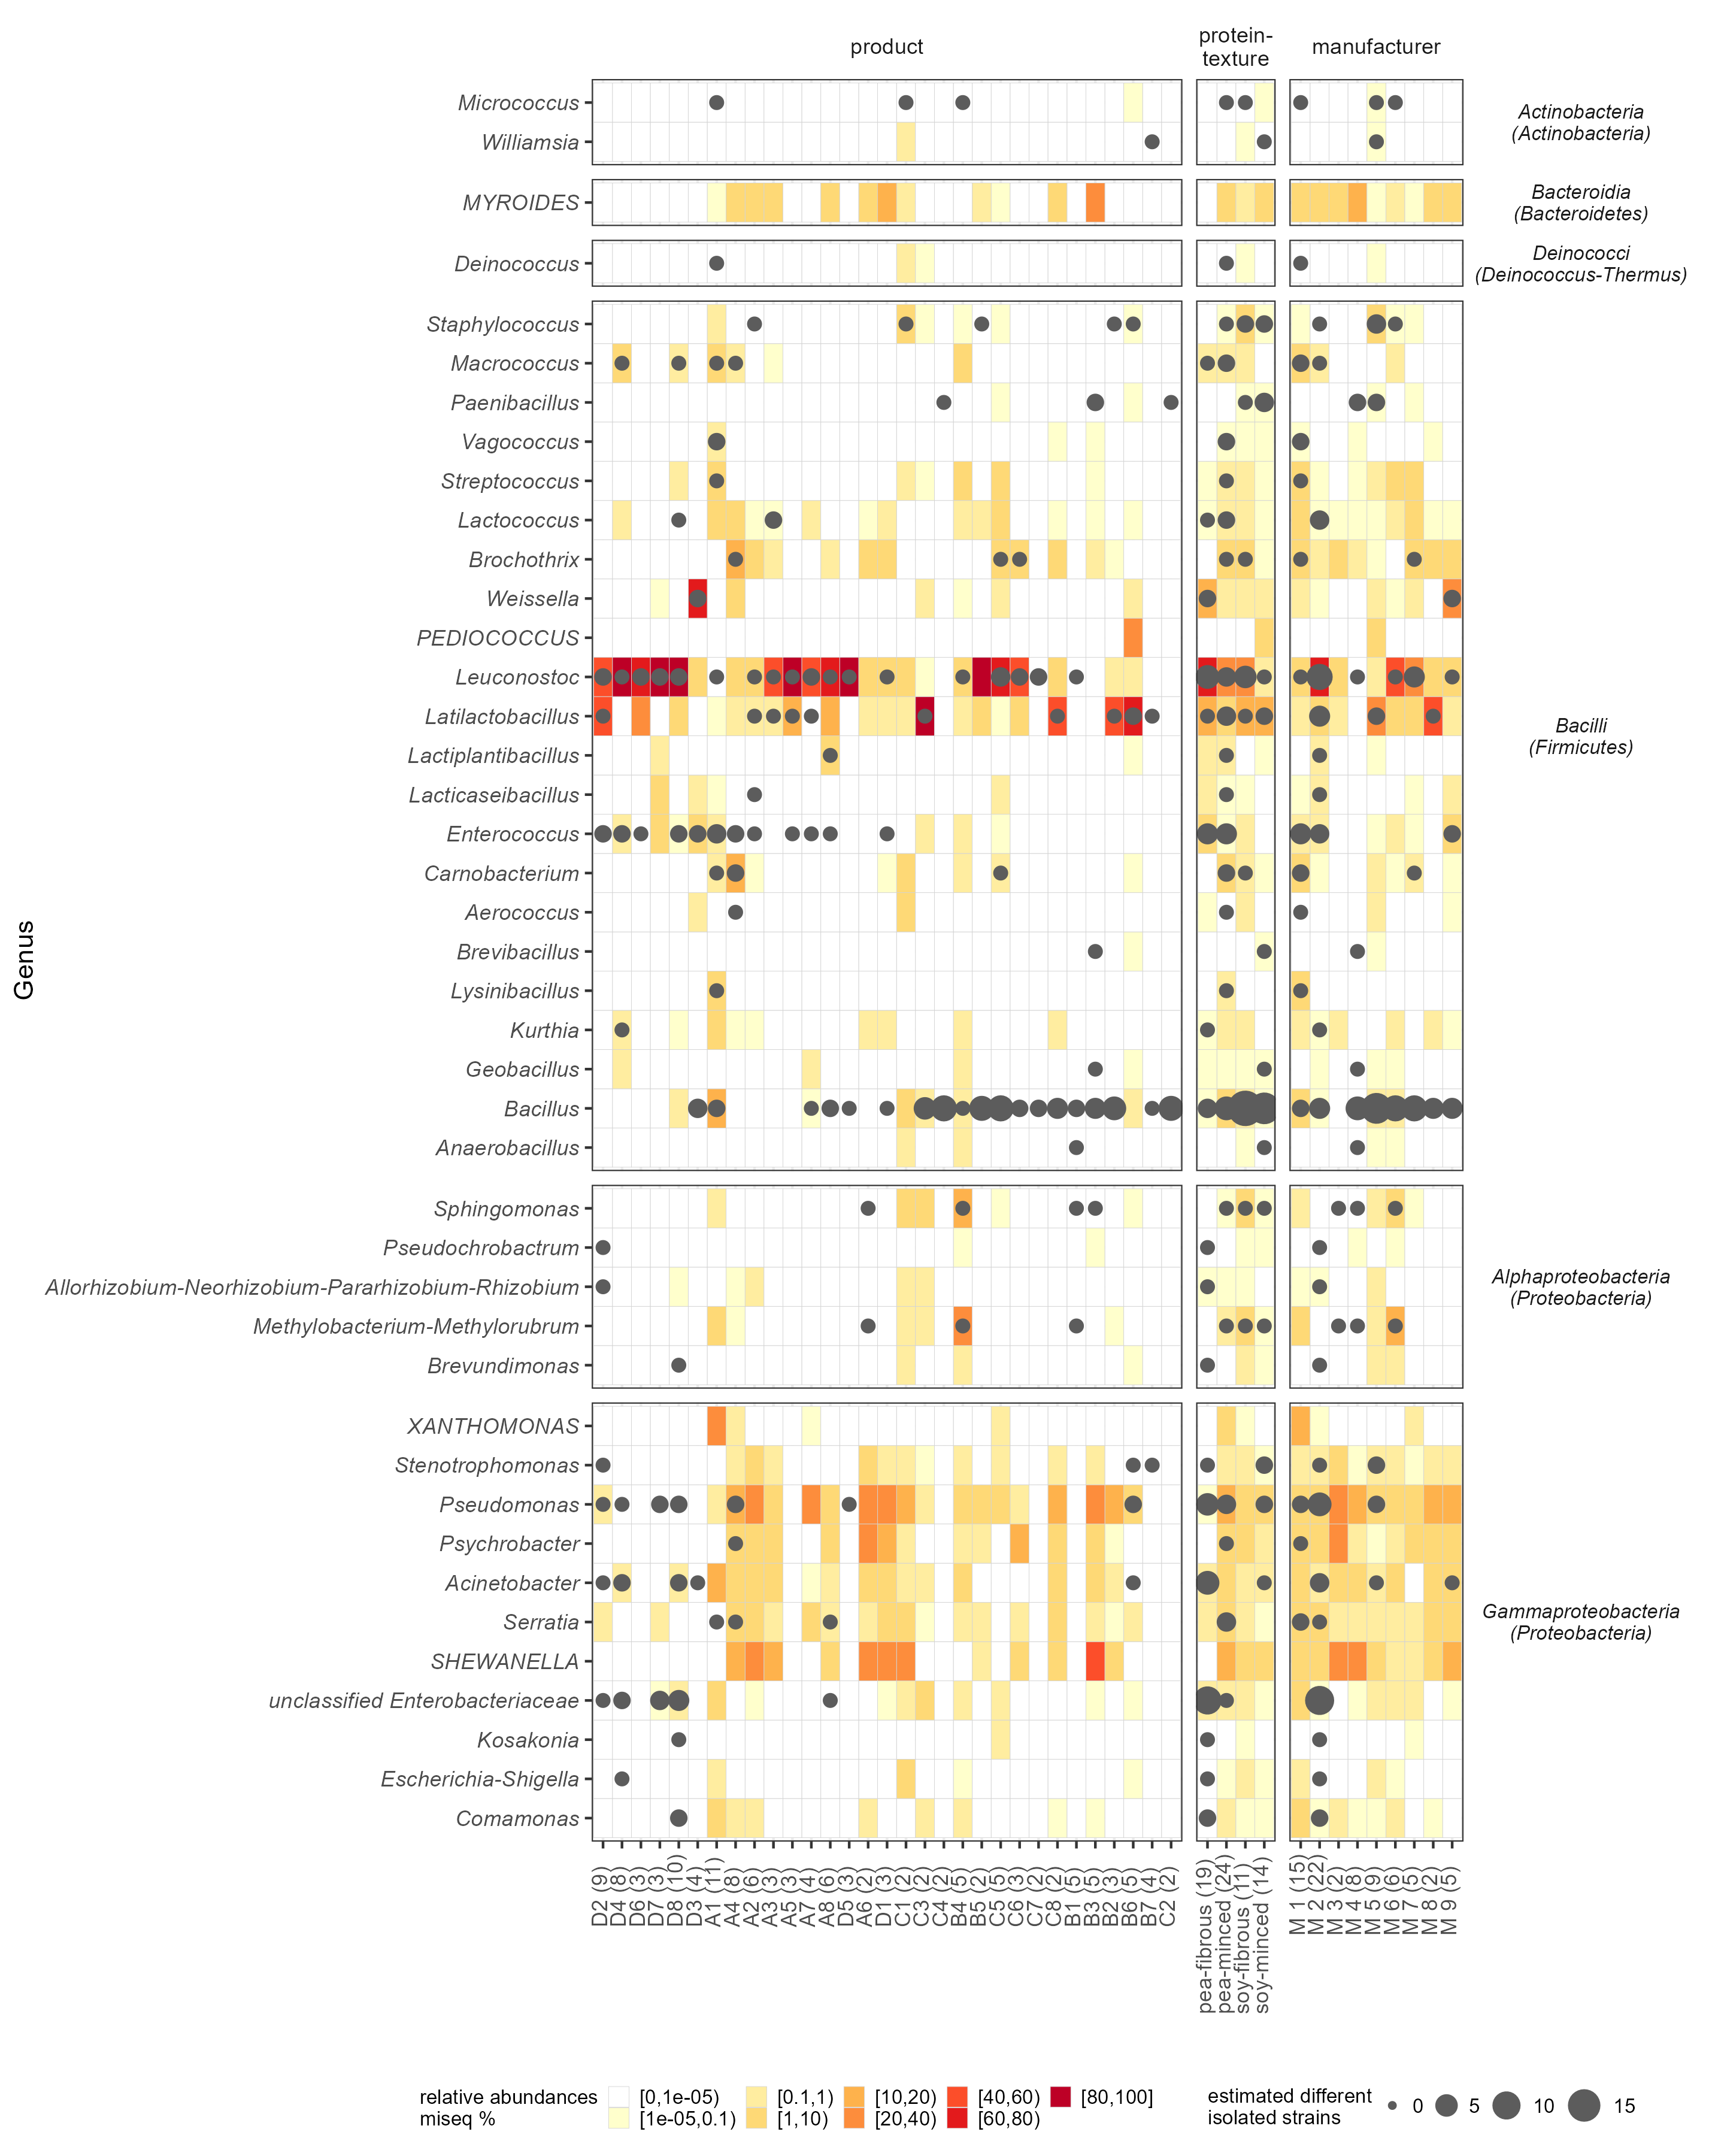
\includegraphics[width=1\linewidth]{Fig1inclmeanrelab} 

}

\caption{\label{fig1} Present isolates per sample, group or manufacturer are represented by dots. Isolates with a genus were clustered based on their 16S rRNA gene sequences. Different clusters represents different strains or species. The higher the number of clusters within a genus, the larger the plotted dot in the figure. The surrounding area is shaded according to the relative abundances in the amplicon sequencing (for the group and manufacturer summary, the mean relative abundance of each included sample is used).}\label{fig:fig1}
\end{figure}

\begin{figure}

{\centering 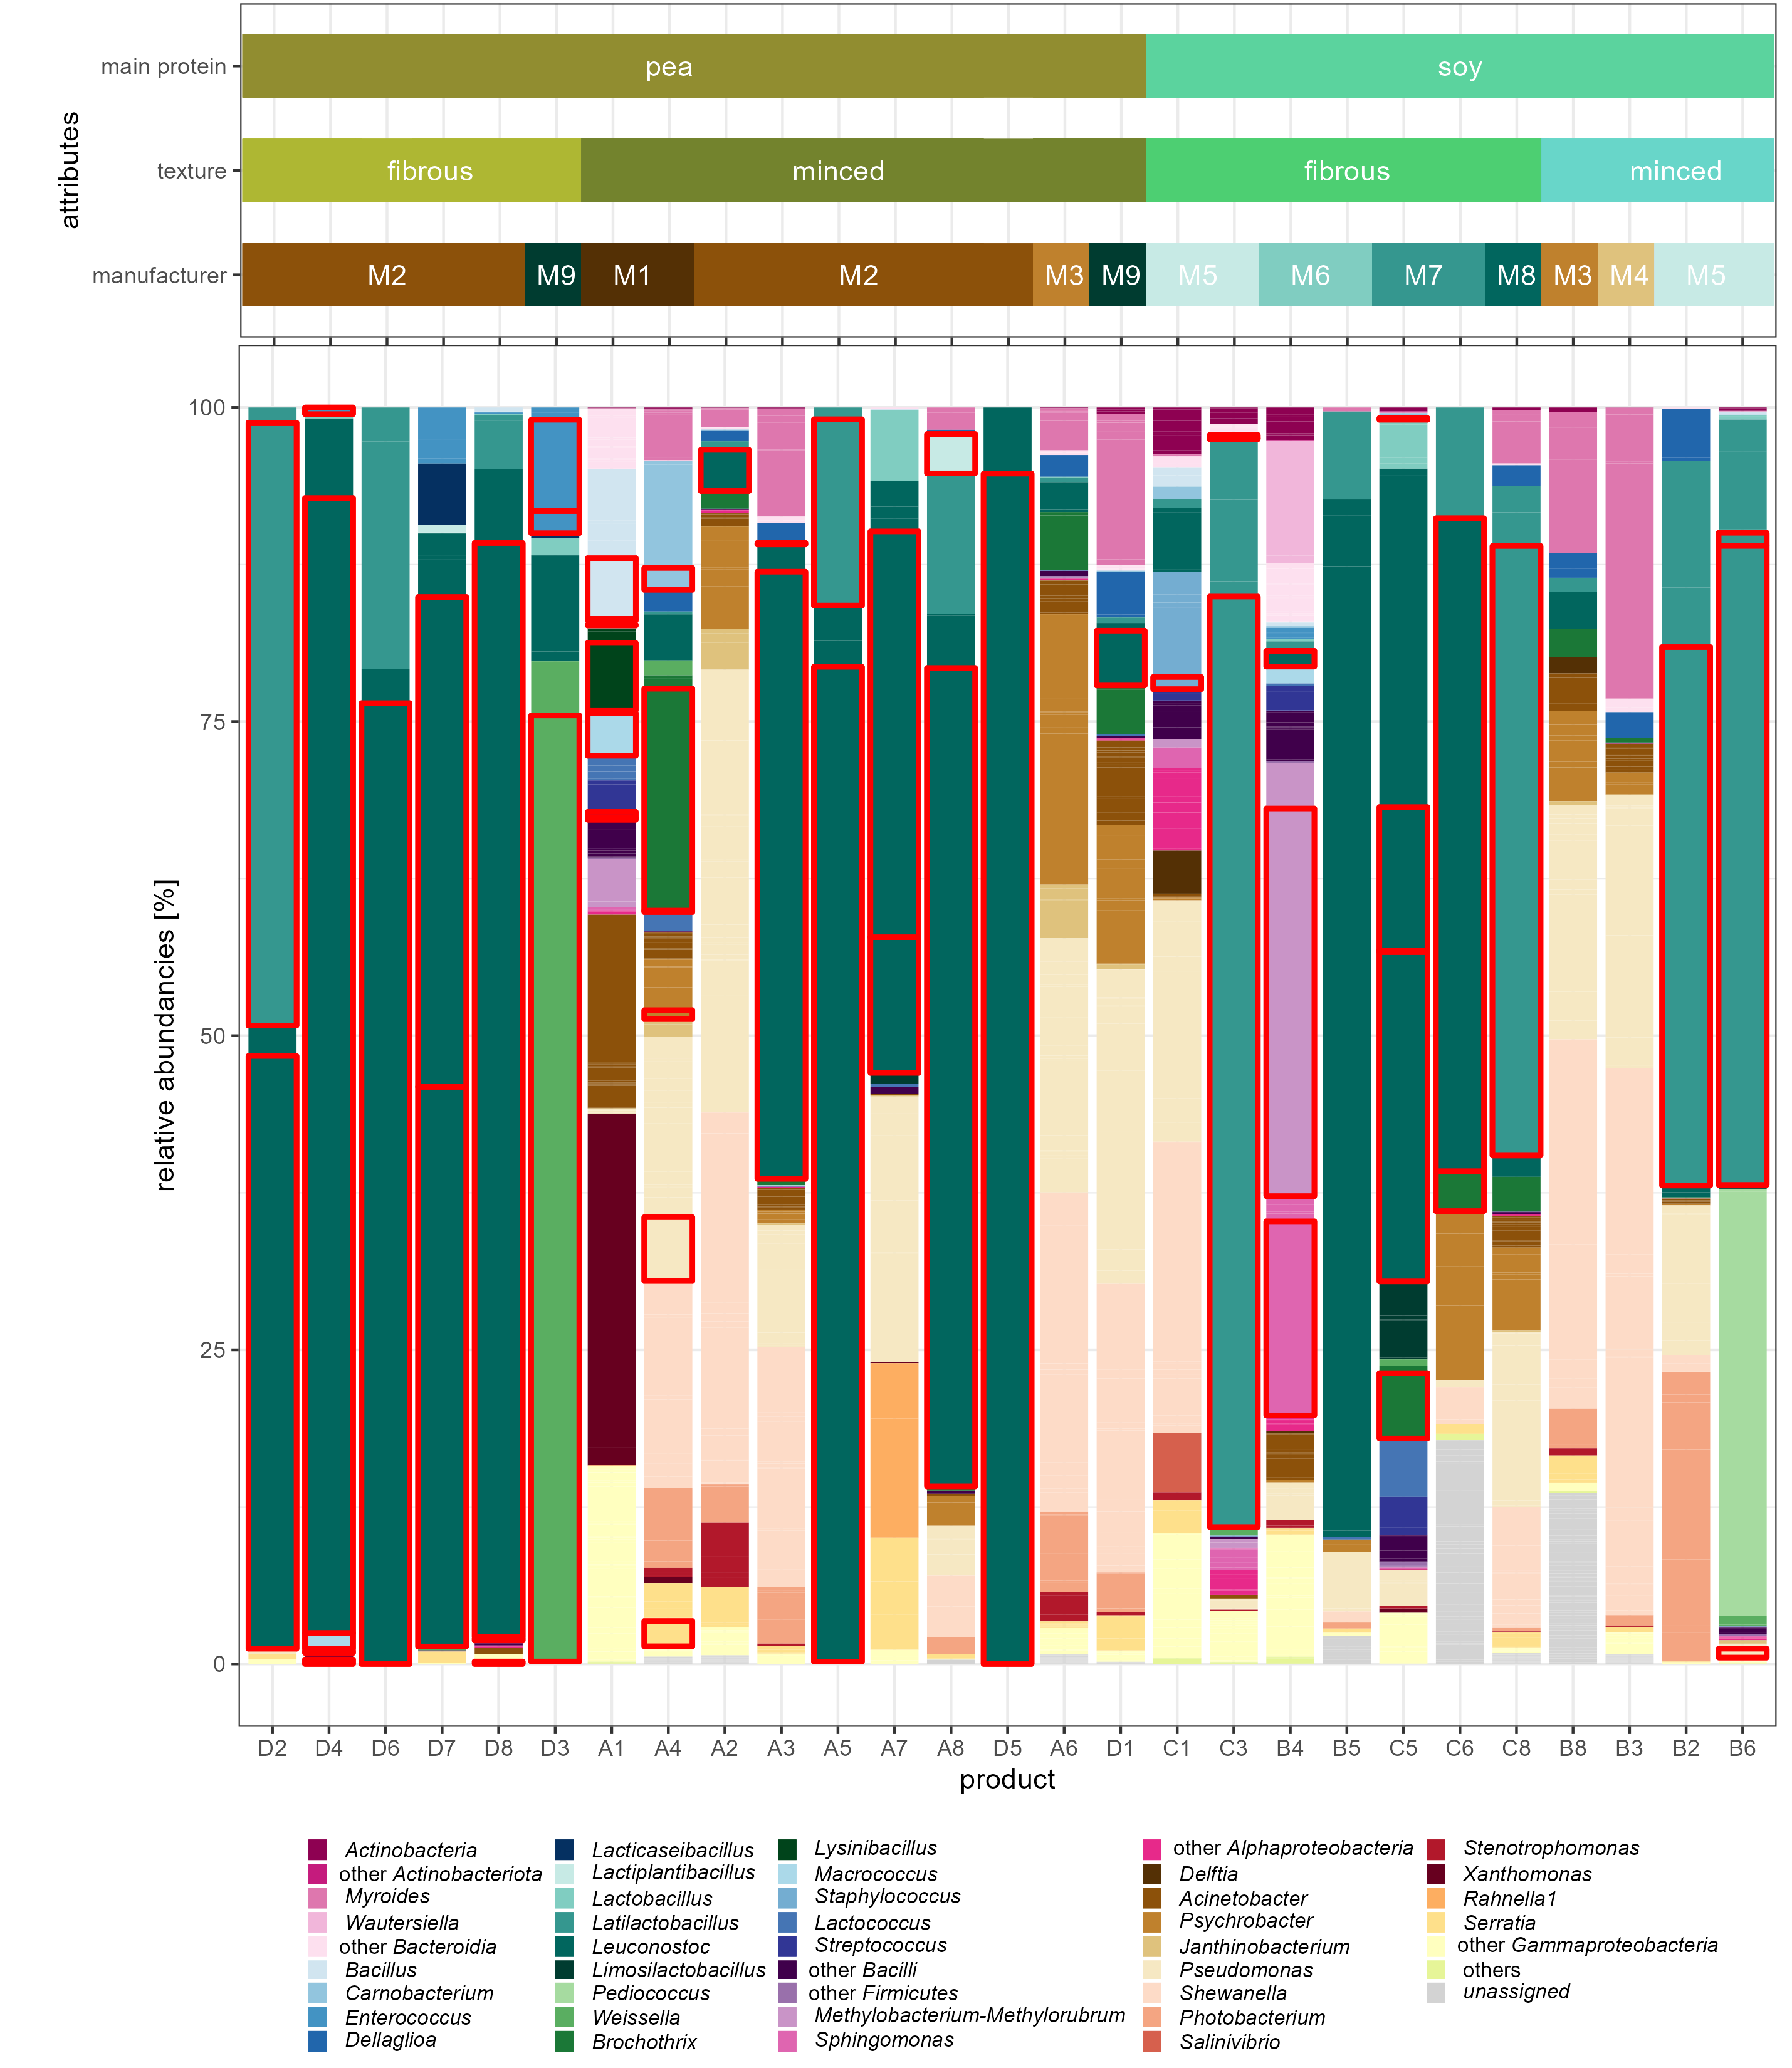
\includegraphics[width=1\linewidth]{Fig2_3percent} 

}

\caption{\label{fig2} Taxonomy plot based on amplicon sequencing, showing the relative abundances on genus level. The underlying relative frequencies of the ASVs are recognizable as pale yellow lines within a genus. Genera with a maximum value of 3\% across all samples were subsumed by color in the next higher taxonomic level.  The samples are ordered by main protein source, texture and manufacturer. ASVs with matching isolates (>99\% identity), were outlined in red.}\label{fig:fig2}
\end{figure}

\begin{figure}

{\centering 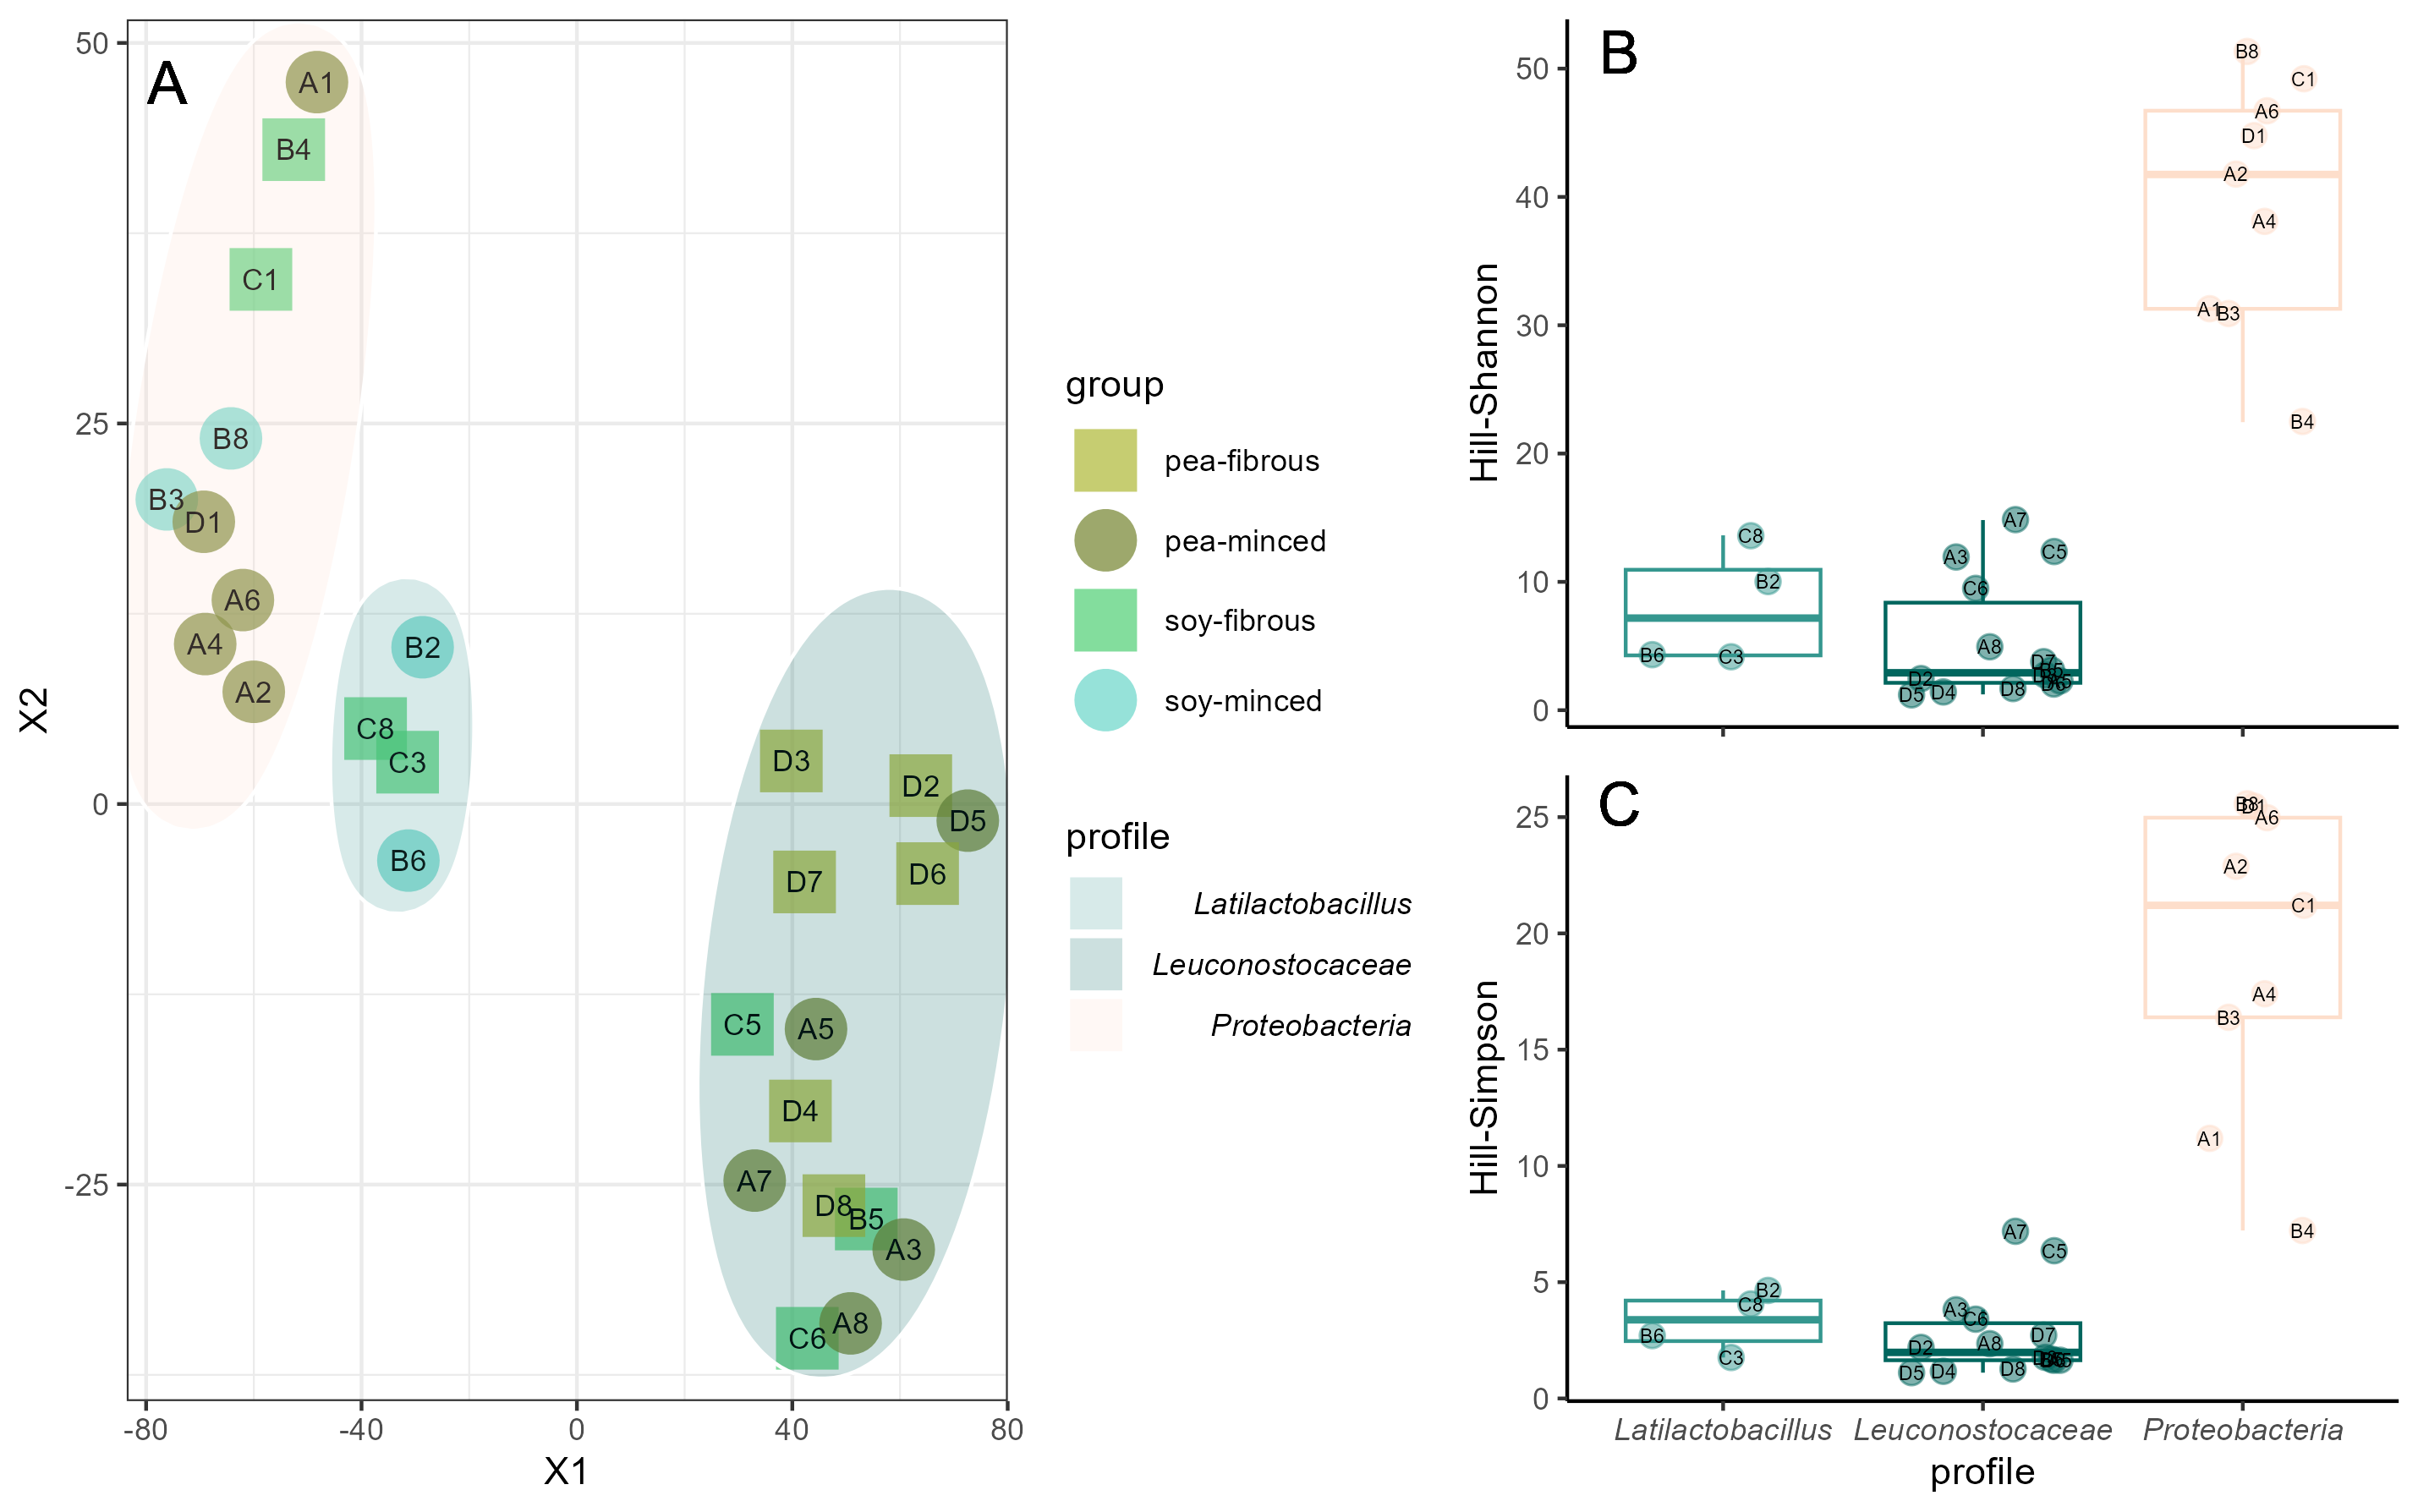
\includegraphics[width=1\linewidth]{Fig3profiles} 

}

\caption{\label{fig3} \textbf {A:} tSNE plot clustered samples to different profiles based on Bray-Curtis dissimilarity (Similar clusters were also found with other distance matrices - see Supplements \ref{figSM4}). \textbf {B:} Hill-Shannon diversity and \textbf {C:} Hill-Simpson diversity comparing these profiles. }\label{fig:fig3}
\end{figure}

\newpage

\hypertarget{supplementary-material}{%
\section*{Supplementary material}\label{supplementary-material}}
\addcontentsline{toc}{section}{Supplementary material}

\beginsupplement

\hypertarget{supplements}{%
\section{Supplements}\label{supplements}}

Supplement Table \ref{tabSM1}:

Supplement Table \ref{tabSM2}: CARD, VFDB, BTyper, AntiSMASH

Supplement \ref{figSM1}: Groupwise comparison of the alpha-diversity
using Hill-Shannon and Hill-Simpson indices. Hill-Shannon index differed
significantly between fibrous and minced pea products (p-val=0.016).

Supplement \ref{figSM2}: NMDS plots using different distance methods.

Supplement \ref{figSM3}: tSNE plots based on Bray-Curtis dissimilarity,
Jaccard distance and Jensen-Shannon divergence. In all three methods,
the same clusters form.

Supplement \ref{figSM4}: LEfSe per group

Supplement \ref{figSM5}: LEfSe per profile.

\singlespacing

\begin{longtable}[b]{llllll}
\caption{\label{tab:tabSM1}\label{tabSM1}PERMANOVA results based on different distance matrices.}\\
\toprule
 & Df & Sum of Sqs & R2 & F & Pr. F\\
\midrule
\endfirsthead
\caption[]{\label{tabSM1}PERMANOVA results based on different distance matrices. \textit{(continued)}}\\
\toprule
 & Df & Sum of Sqs & R2 & F & Pr. F\\
\midrule
\endhead

\endfoot
\bottomrule
\endlastfoot
\addlinespace[0.3em]
\multicolumn{6}{l}{\textbf{Bray-Curtis}}\\
\addlinespace[0.3em]
\multicolumn{6}{l}{\textit{\makecell[l]{Permutation test for adonis under reduced model\\Terms added sequentially (first to last)\\Permutation: free\\Number of permutations: 999\\adonis2(formula = dmlistshort[[i]] \textasciitilde{} protein.source * texture,\\data = data.frame(sample\_data(relab\_po)), permutations = 999)}}}\\
\hspace{1em}\hspace{1em}protein source & 1 & 0.7258 & 0.0743 & 2.090 & 0.030\\
\hspace{1em}\hspace{1em}texture & 1 & 0.8391 & 0.0859 & 2.416 & 0.017\\
\hspace{1em}\hspace{1em}protein source:texture & 1 & 0.2185 & 0.0224 & 0.629 & 0.825\\
\hspace{1em}\hspace{1em}residual & 23 & 7.9874 & 0.8175 &  \vphantom{1} & \\
\hspace{1em}\hspace{1em}total & 26 & 9.7708 & 1.0000 &  \vphantom{1} & \\
\addlinespace[0.3em]
\multicolumn{6}{l}{\textit{\makecell[l]{Permutation test for adonis under reduced model\\Terms added sequentially (first to last)\\Permutation: free\\Number of permutations: 999\\adonis2(formula = dmlistshort[[i]] \textasciitilde{} texture * protein.source,\\data = data.frame(sample\_data(relab\_po)), permutations = 999)}}}\\
\hspace{1em}\hspace{1em}protein source & 1 & 0.6784 & 0.0694 & 1.953 & 0.041\\
\hspace{1em}\hspace{1em}texture & 1 & 0.8864 & 0.0907 & 2.553 & 0.017\\
\hspace{1em}\hspace{1em}protein source:texture & 1 & 0.2185 & 0.0224 & 0.629 & 0.834\\
\hspace{1em}\hspace{1em}residual & 23 & 7.9874 & 0.8175 &  & \\
\hspace{1em}\hspace{1em}total & 26 & 9.7708 & 1.0000 &  & \\
\addlinespace[0.3em]
\multicolumn{6}{l}{\textbf{Jaccard}}\\
\addlinespace[0.3em]
\multicolumn{6}{l}{\textit{\makecell[l]{Permutation test for adonis under reduced model\\Terms added sequentially (first to last)\\Permutation: free\\Number of permutations: 999\\adonis2(formula = dmlistshort[[i]] \textasciitilde{} protein.source * texture,\\data = data.frame(sample\_data(relab\_po)), permutations = 999)}}}\\
\hspace{1em}\hspace{1em}protein source & 1 & 0.6774 & 0.0626 & 1.712 & 0.041\\
\hspace{1em}\hspace{1em}texture & 1 & 0.7484 & 0.0691 & 1.891 & 0.022\\
\hspace{1em}\hspace{1em}protein source:texture & 1 & 0.3001 & 0.0277 & 0.758 & 0.789\\
\hspace{1em}\hspace{1em}residual & 23 & 9.1035 & 0.8406 &  \vphantom{1} & \\
\hspace{1em}\hspace{1em}total & 26 & 10.8295 & 1.0000 &  \vphantom{1} & \\
\addlinespace[0.3em]
\multicolumn{6}{l}{\textit{\makecell[l]{Permutation test for adonis under reduced model\\Terms added sequentially (first to last)\\Permutation: free\\Number of permutations: 999\\adonis2(formula = dmlistshort[[i]] \textasciitilde{} texture * protein.source,\\data = data.frame(sample\_data(relab\_po)), permutations = 999)}}}\\
\hspace{1em}\hspace{1em}protein source & 1 & 0.6367 & 0.0588 & 1.609 & 0.065\\
\hspace{1em}\hspace{1em}texture & 1 & 0.7891 & 0.0729 & 1.994 & 0.014\\
\hspace{1em}\hspace{1em}protein source:texture & 1 & 0.3001 & 0.0277 & 0.758 & 0.770\\
\hspace{1em}\hspace{1em}residual & 23 & 9.1035 & 0.8406 &  & \\
\hspace{1em}\hspace{1em}total & 26 & 10.8295 & 1.0000 &  & \\
\addlinespace[0.3em]
\multicolumn{6}{l}{\textbf{Jensen-Shannon}}\\
\addlinespace[0.3em]
\multicolumn{6}{l}{\textit{\makecell[l]{Permutation test for adonis under reduced model\\Terms added sequentially (first to last)\\Permutation: free\\Number of permutations: 999\\adonis2(formula = dmlistshort[[i]] \textasciitilde{} protein.source * texture,\\data = data.frame(sample\_data(relab\_po)), permutations = 999)}}}\\
\hspace{1em}\hspace{1em}protein source & 1 & 0.3254 & 0.0874 & 2.626 & 0.034\\
\hspace{1em}\hspace{1em}texture & 1 & 0.4556 & 0.1224 & 3.676 & 0.008\\
\hspace{1em}\hspace{1em}protein source:texture & 1 & 0.0918 & 0.0246 & 0.740 & 0.607\\
\hspace{1em}\hspace{1em}residual & 23 & 2.8504 & 0.7656 &  \vphantom{1} & \\
\hspace{1em}\hspace{1em}total & 26 & 3.7231 & 1.0000 &  \vphantom{1} & \\
\addlinespace[0.3em]
\multicolumn{6}{l}{\textit{\makecell[l]{Permutation test for adonis under reduced model\\Terms added sequentially (first to last)\\Permutation: free\\Number of permutations: 999\\adonis2(formula = dmlistshort[[i]] \textasciitilde{} texture * protein.source,\\data = data.frame(sample\_data(relab\_po)), permutations = 999)}}}\\
\hspace{1em}\hspace{1em}protein source & 1 & 0.3698 & 0.0993 & 2.984 & 0.019\\
\hspace{1em}\hspace{1em}texture & 1 & 0.4111 & 0.1104 & 3.318 & 0.007\\
\hspace{1em}\hspace{1em}protein source:texture & 1 & 0.0918 & 0.0246 & 0.740 & 0.609\\
\hspace{1em}\hspace{1em}residual & 23 & 2.8504 & 0.7656 &  & \\
\hspace{1em}\hspace{1em}total & 26 & 3.7231 & 1.0000 &  & \\*
\end{longtable}

\doublespacing

\begin{figure}

{\centering 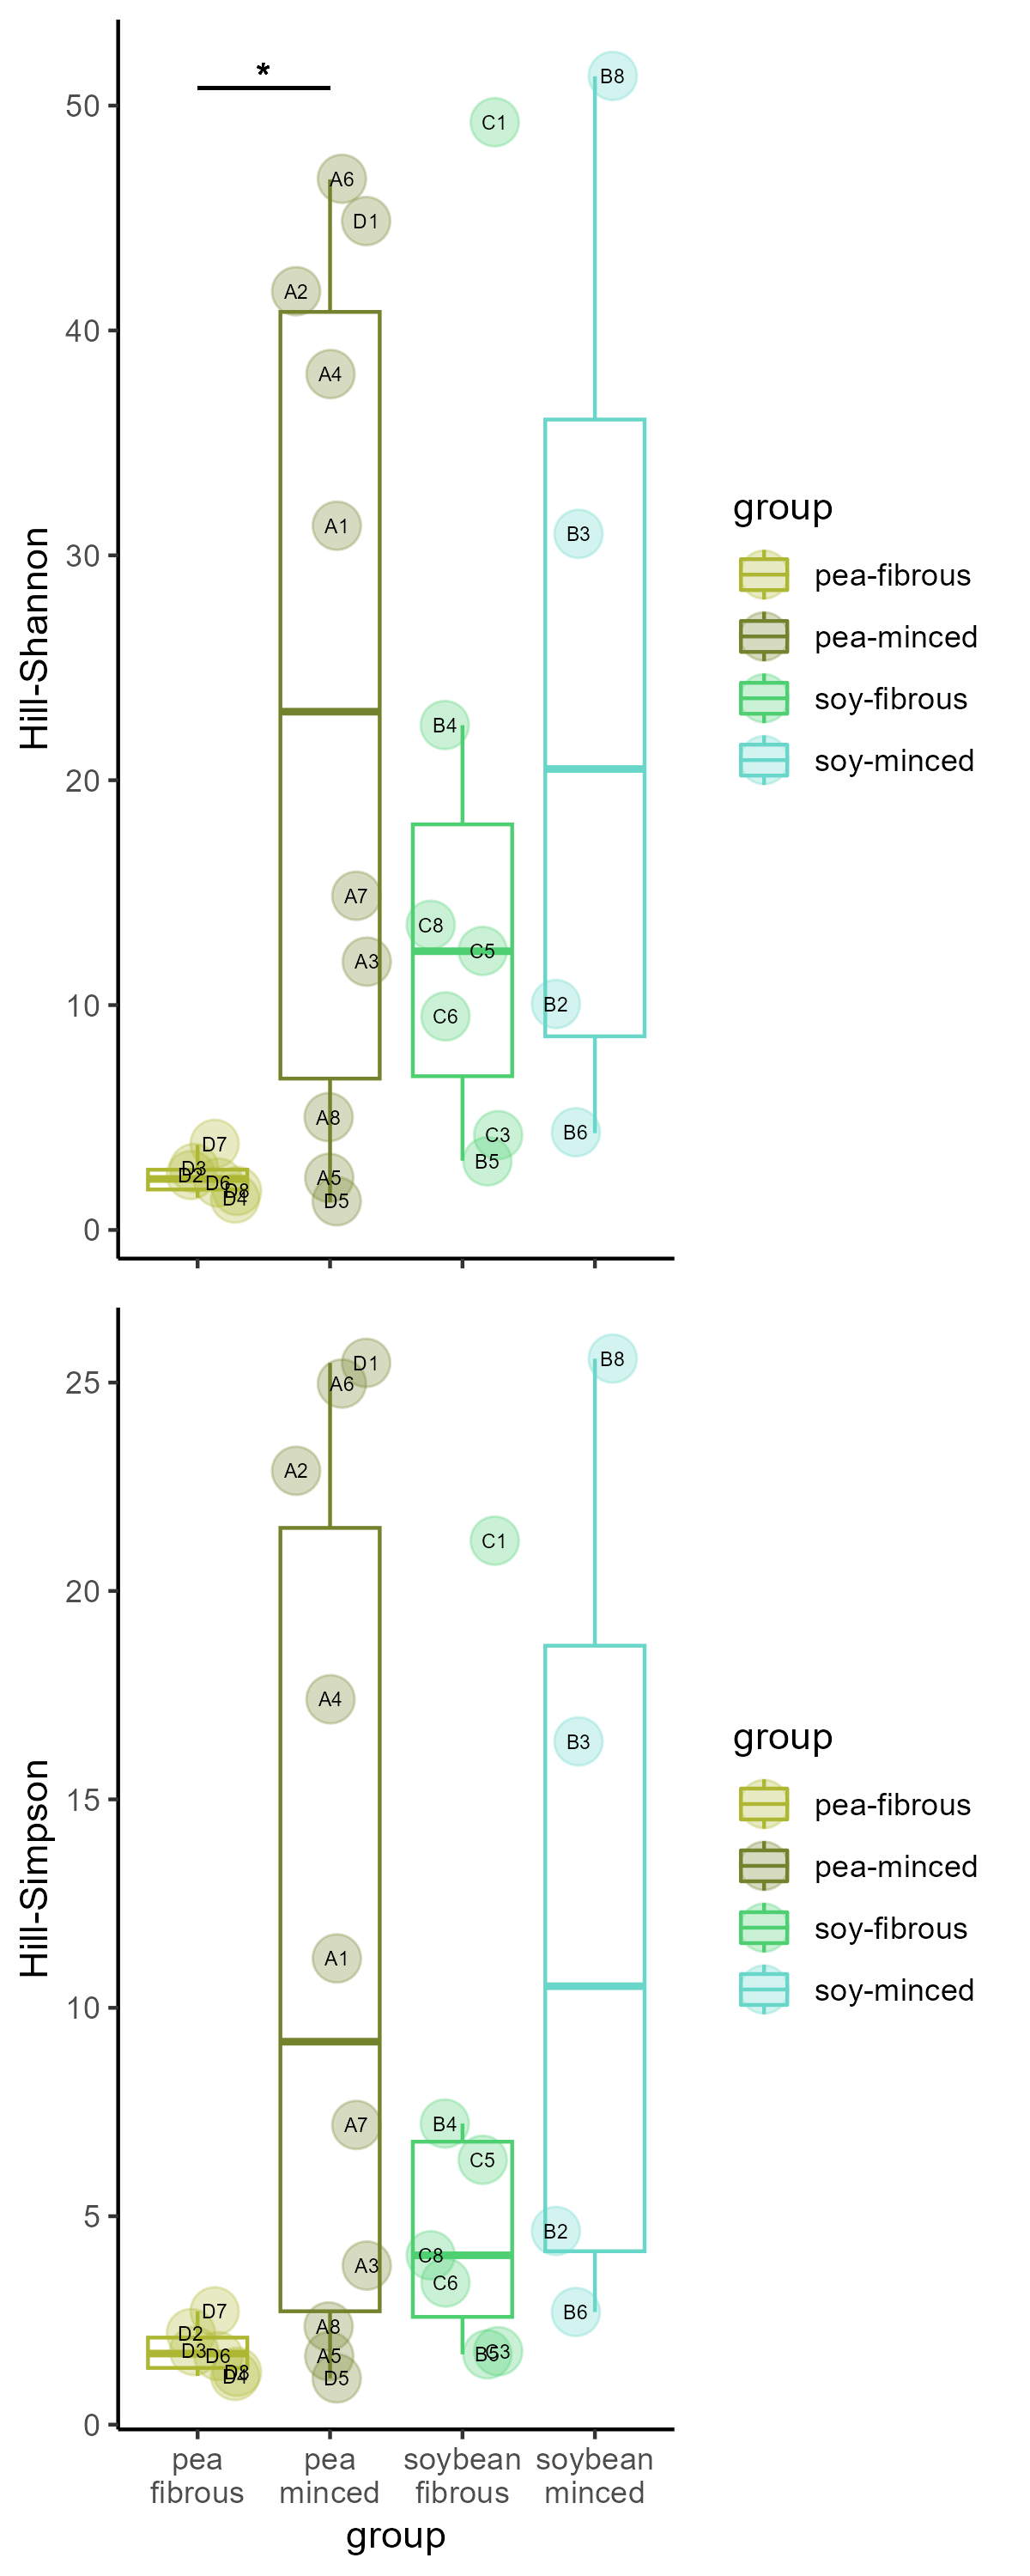
\includegraphics[width=0.5\linewidth]{PlotDivByCov} 

}

\caption{\label{figSM1} Groupwise comparison of the alpha-diversity using Hill-Shannon and Hill-Simpson indices. Hill-Shannon index differed significantly between fibrous and minced pea products (p-val=0.016).}\label{fig:figSM1}
\end{figure}

\begin{figure}

{\centering 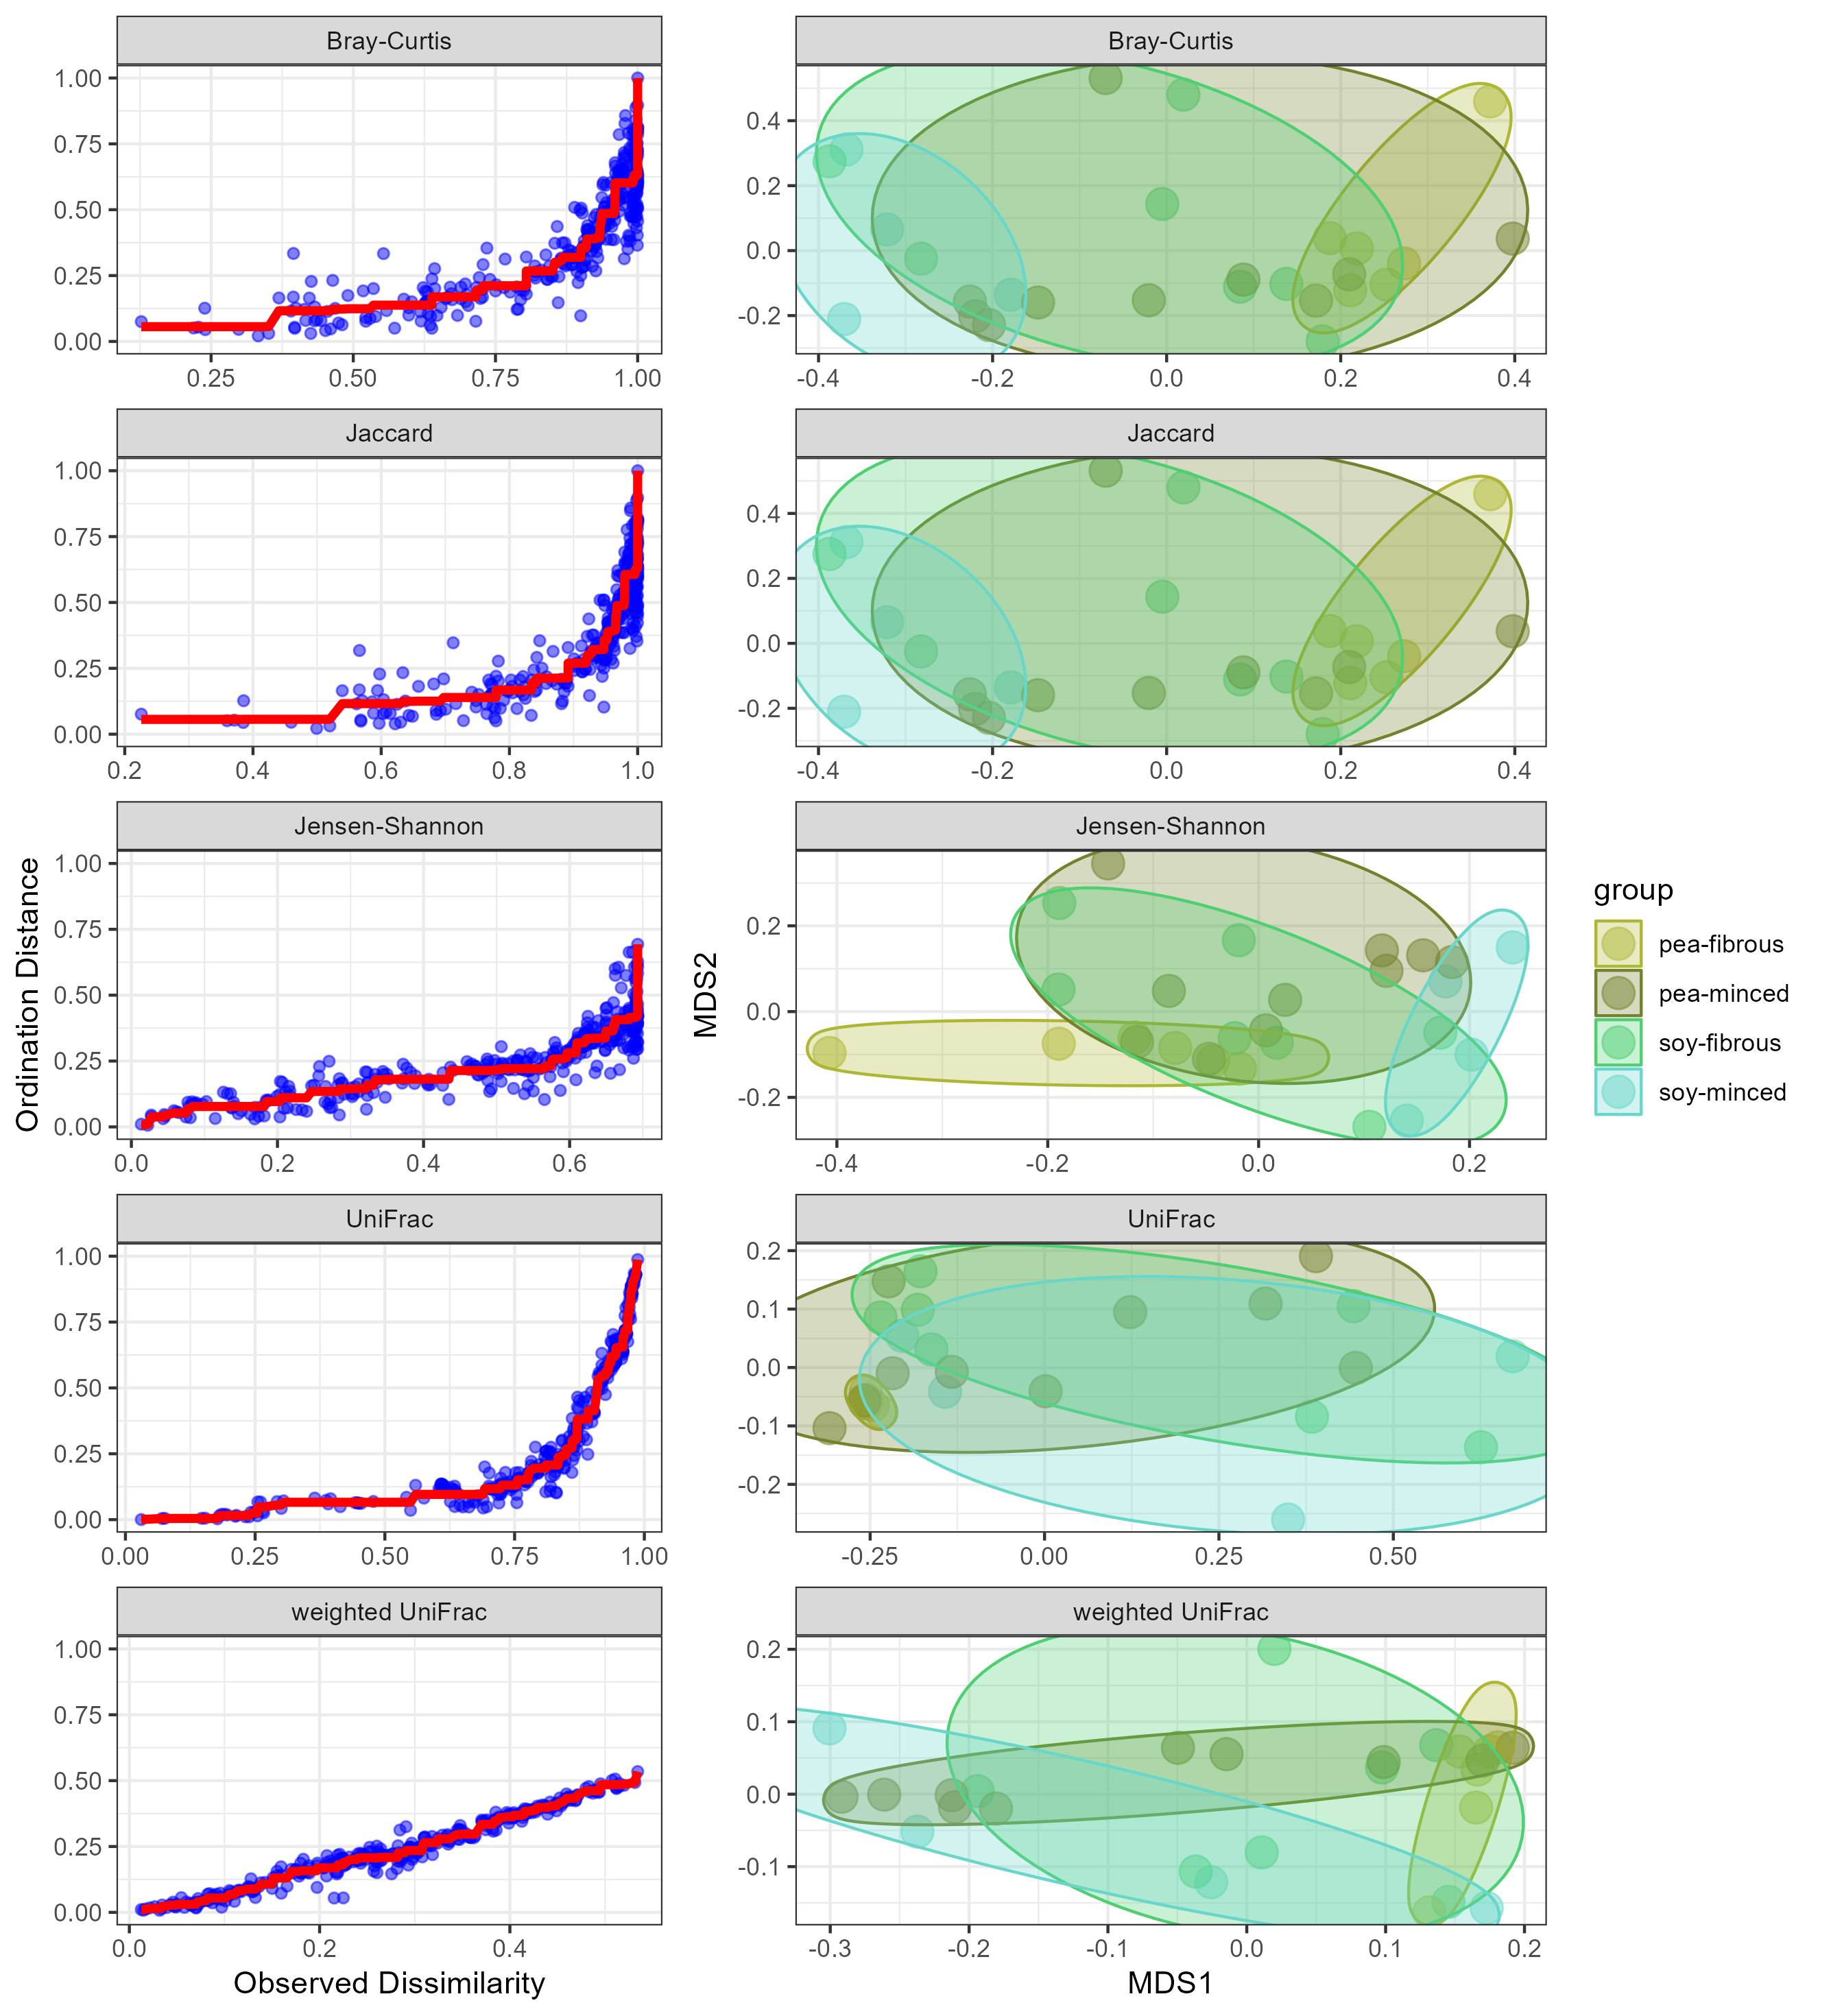
\includegraphics[width=1\linewidth]{NMDSplots} 

}

\caption{\label{figSM2} NMDS plots using different distance methods.  }\label{fig:figSM2}
\end{figure}

\begin{figure}

{\centering 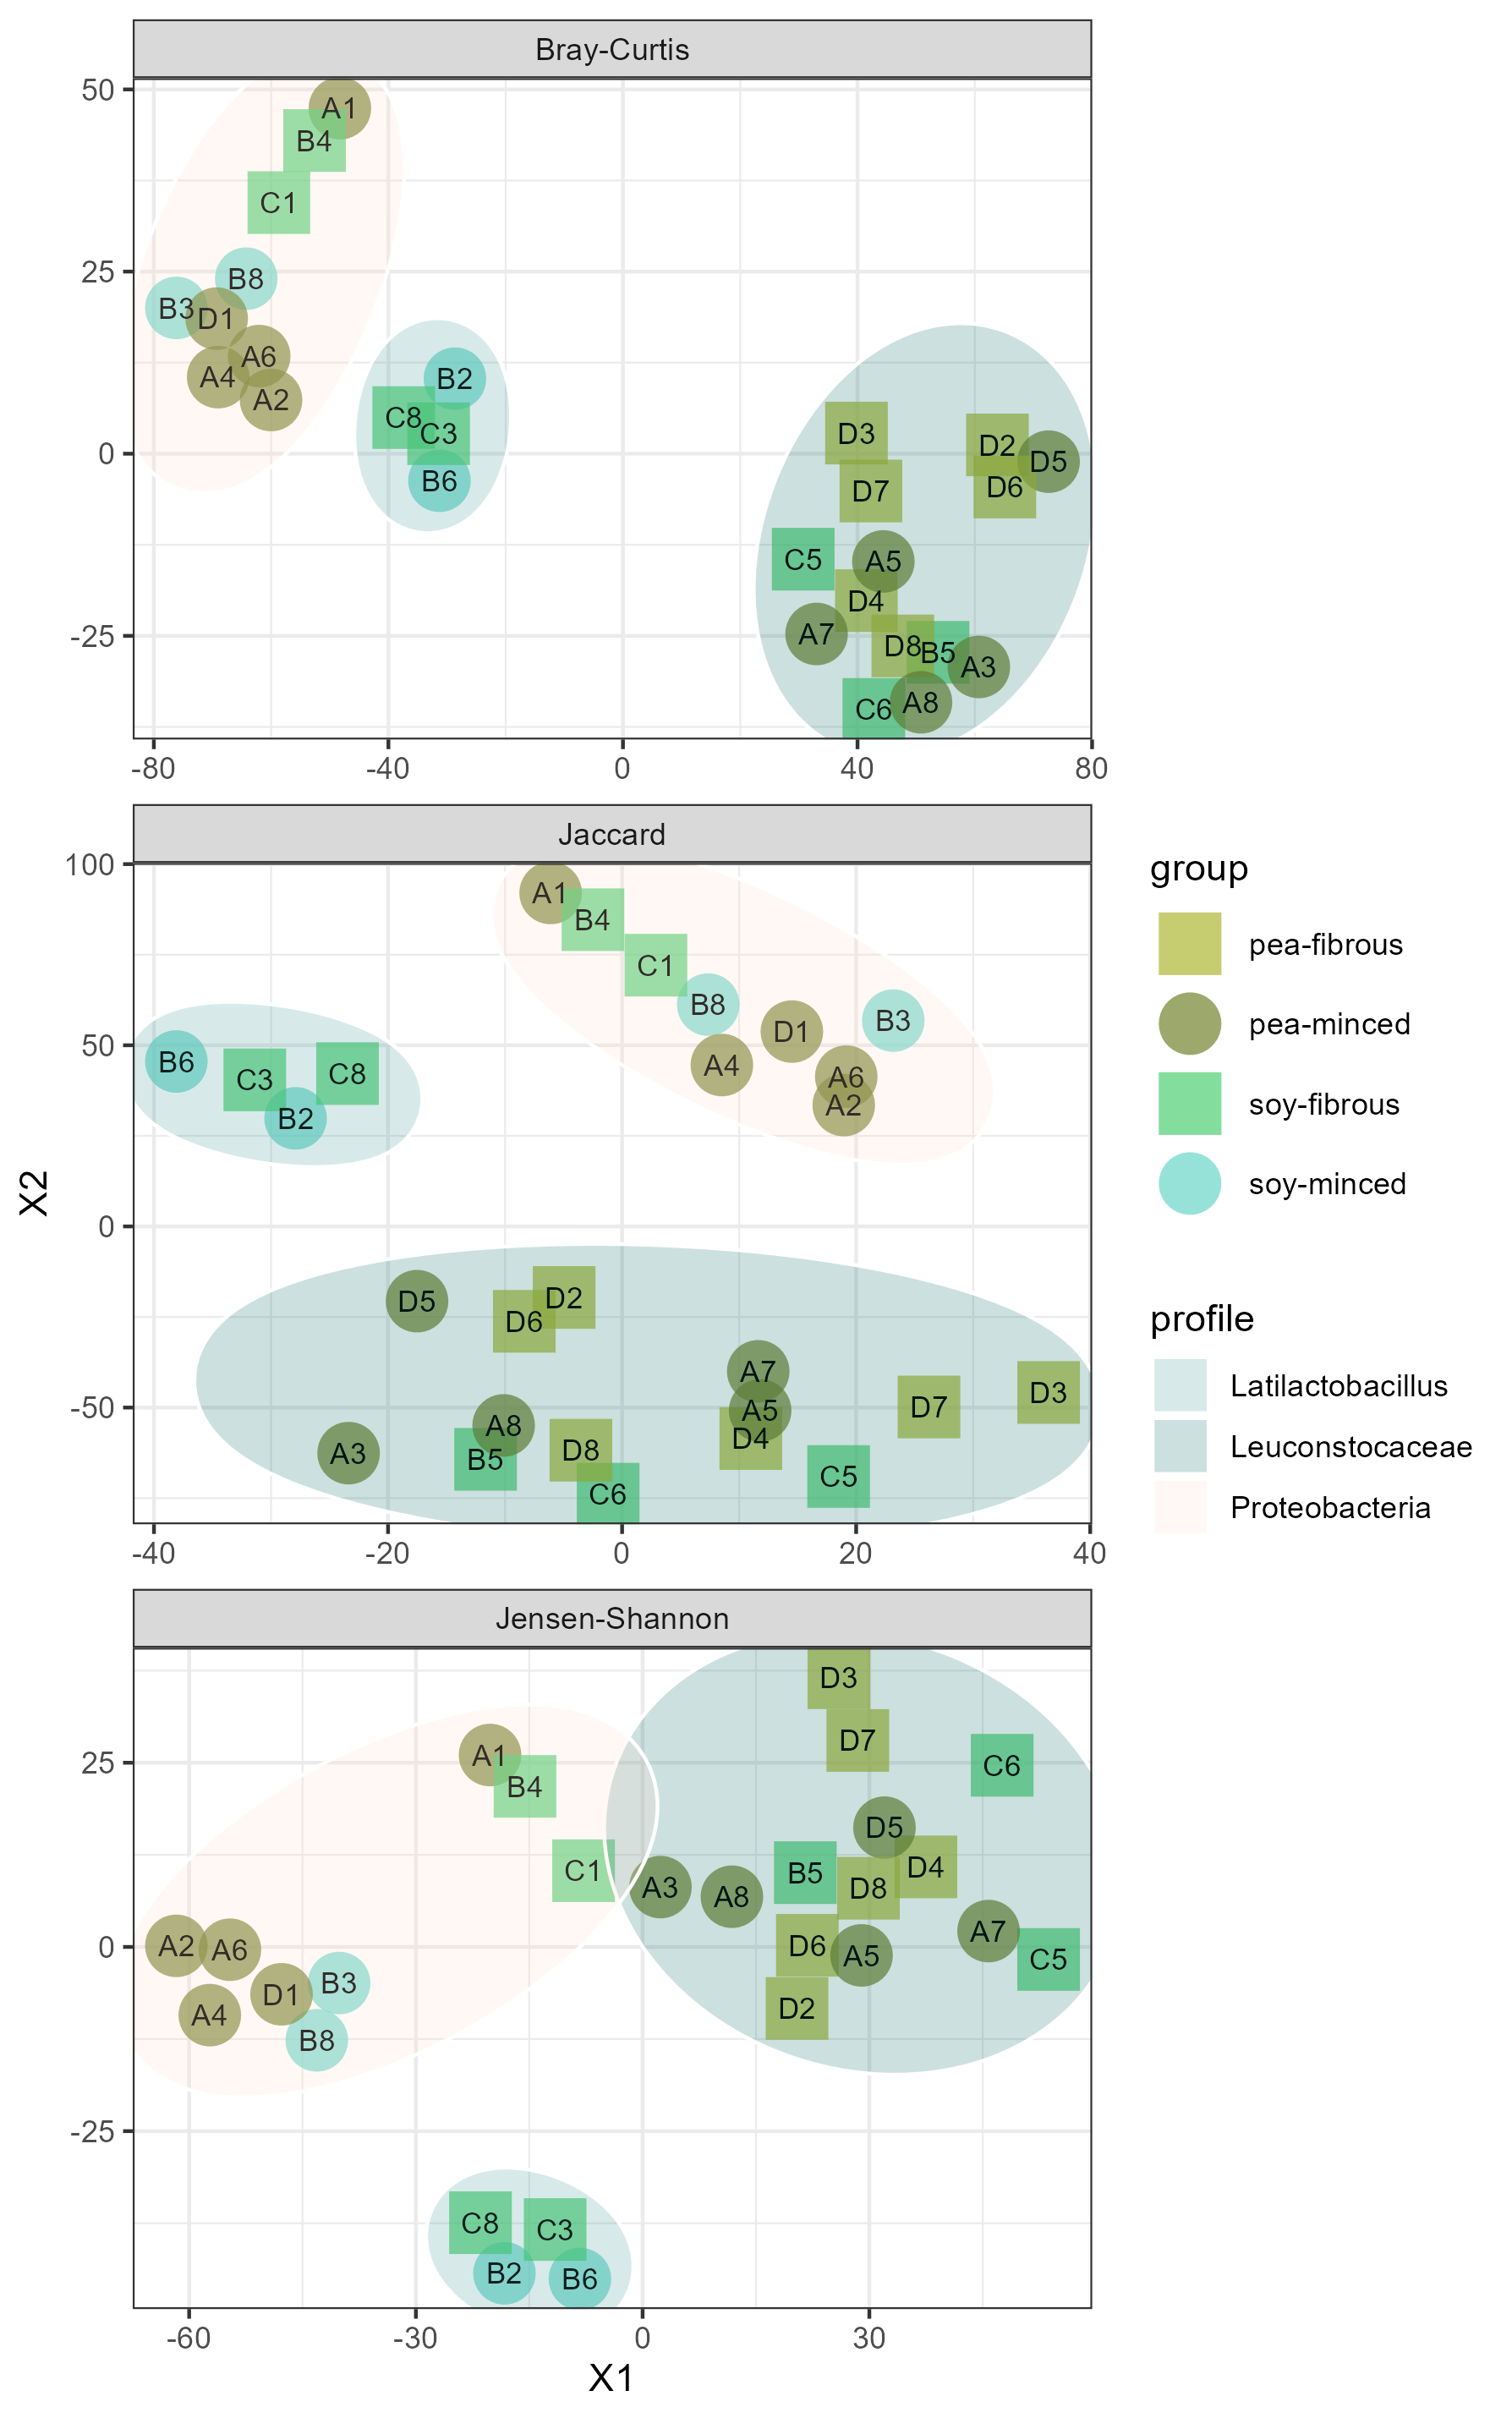
\includegraphics[width=0.8\linewidth]{FigSM4} 

}

\caption{\label{figSM3} tSNE plots based on Bray-Curtis dissimilarity, Jaccard distance and Jensen-Shannon divergence. In all three methods, the same clusters form.  }\label{fig:figSM3}
\end{figure}

\begin{figure}

{\centering 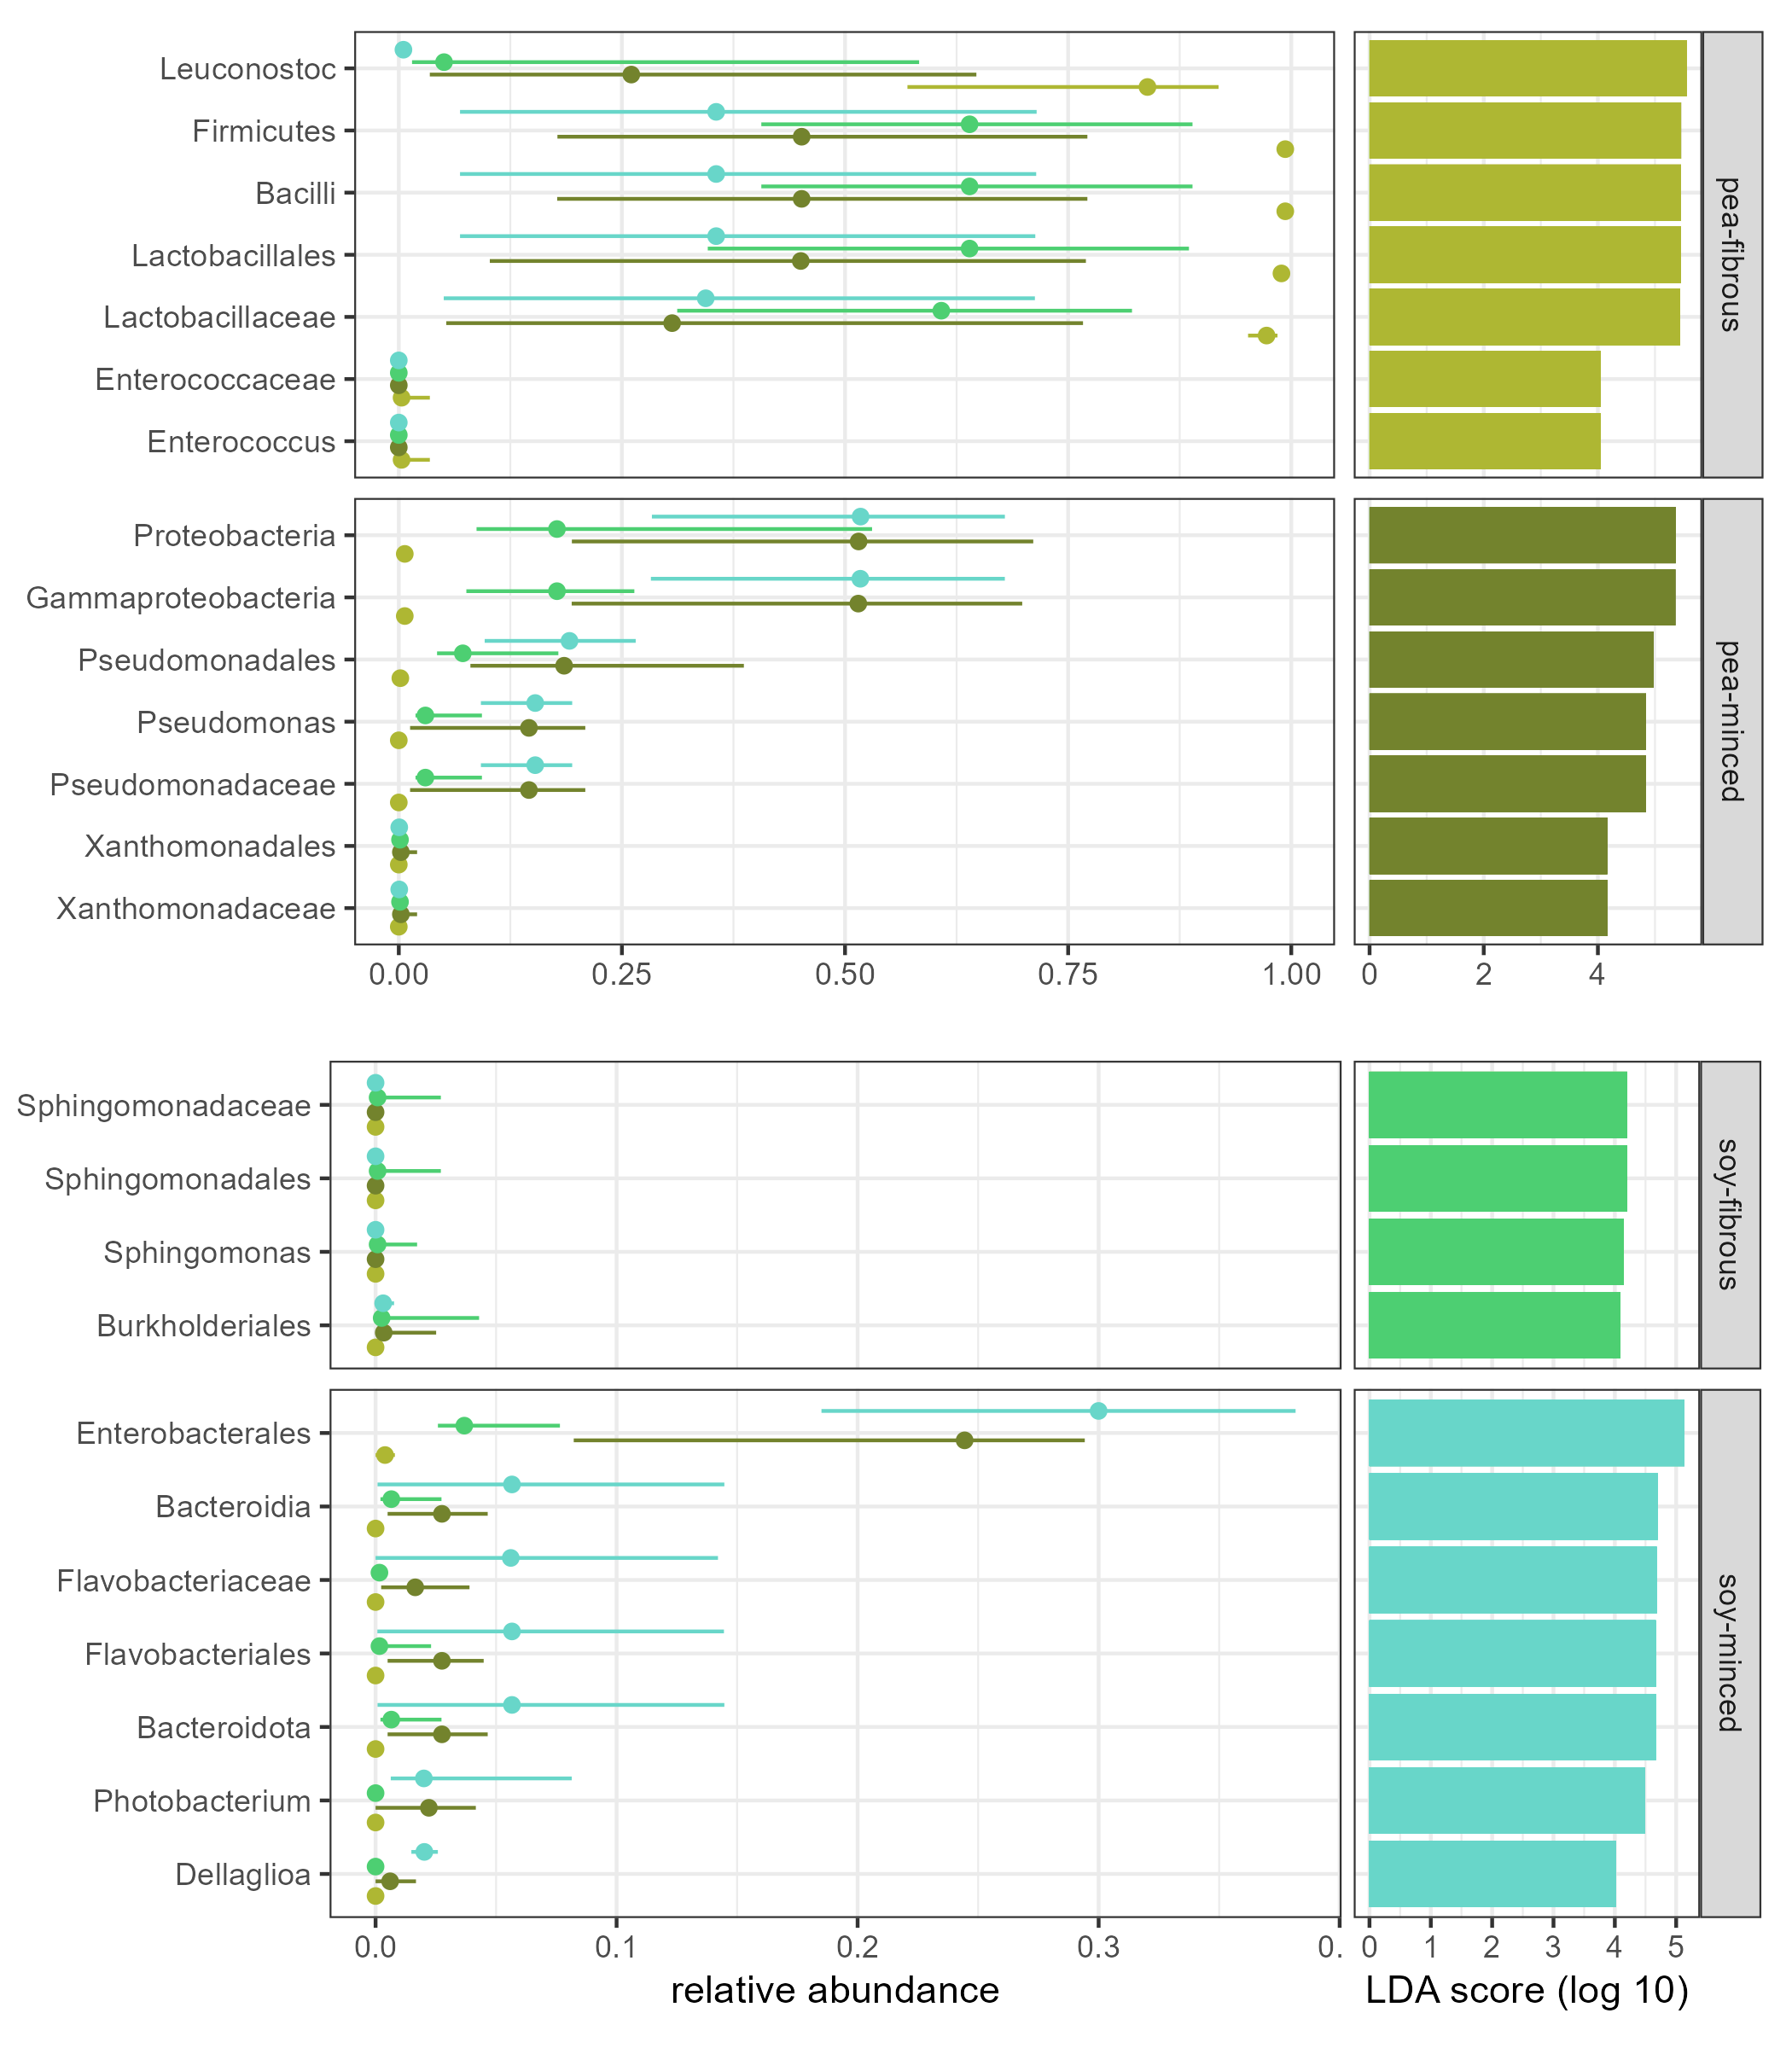
\includegraphics[width=1\linewidth]{lefsestatplotdiffscales} 

}

\caption{\label{figSM4} LEfSe per group.  }\label{fig:figSM4}
\end{figure}

\begin{figure}

{\centering 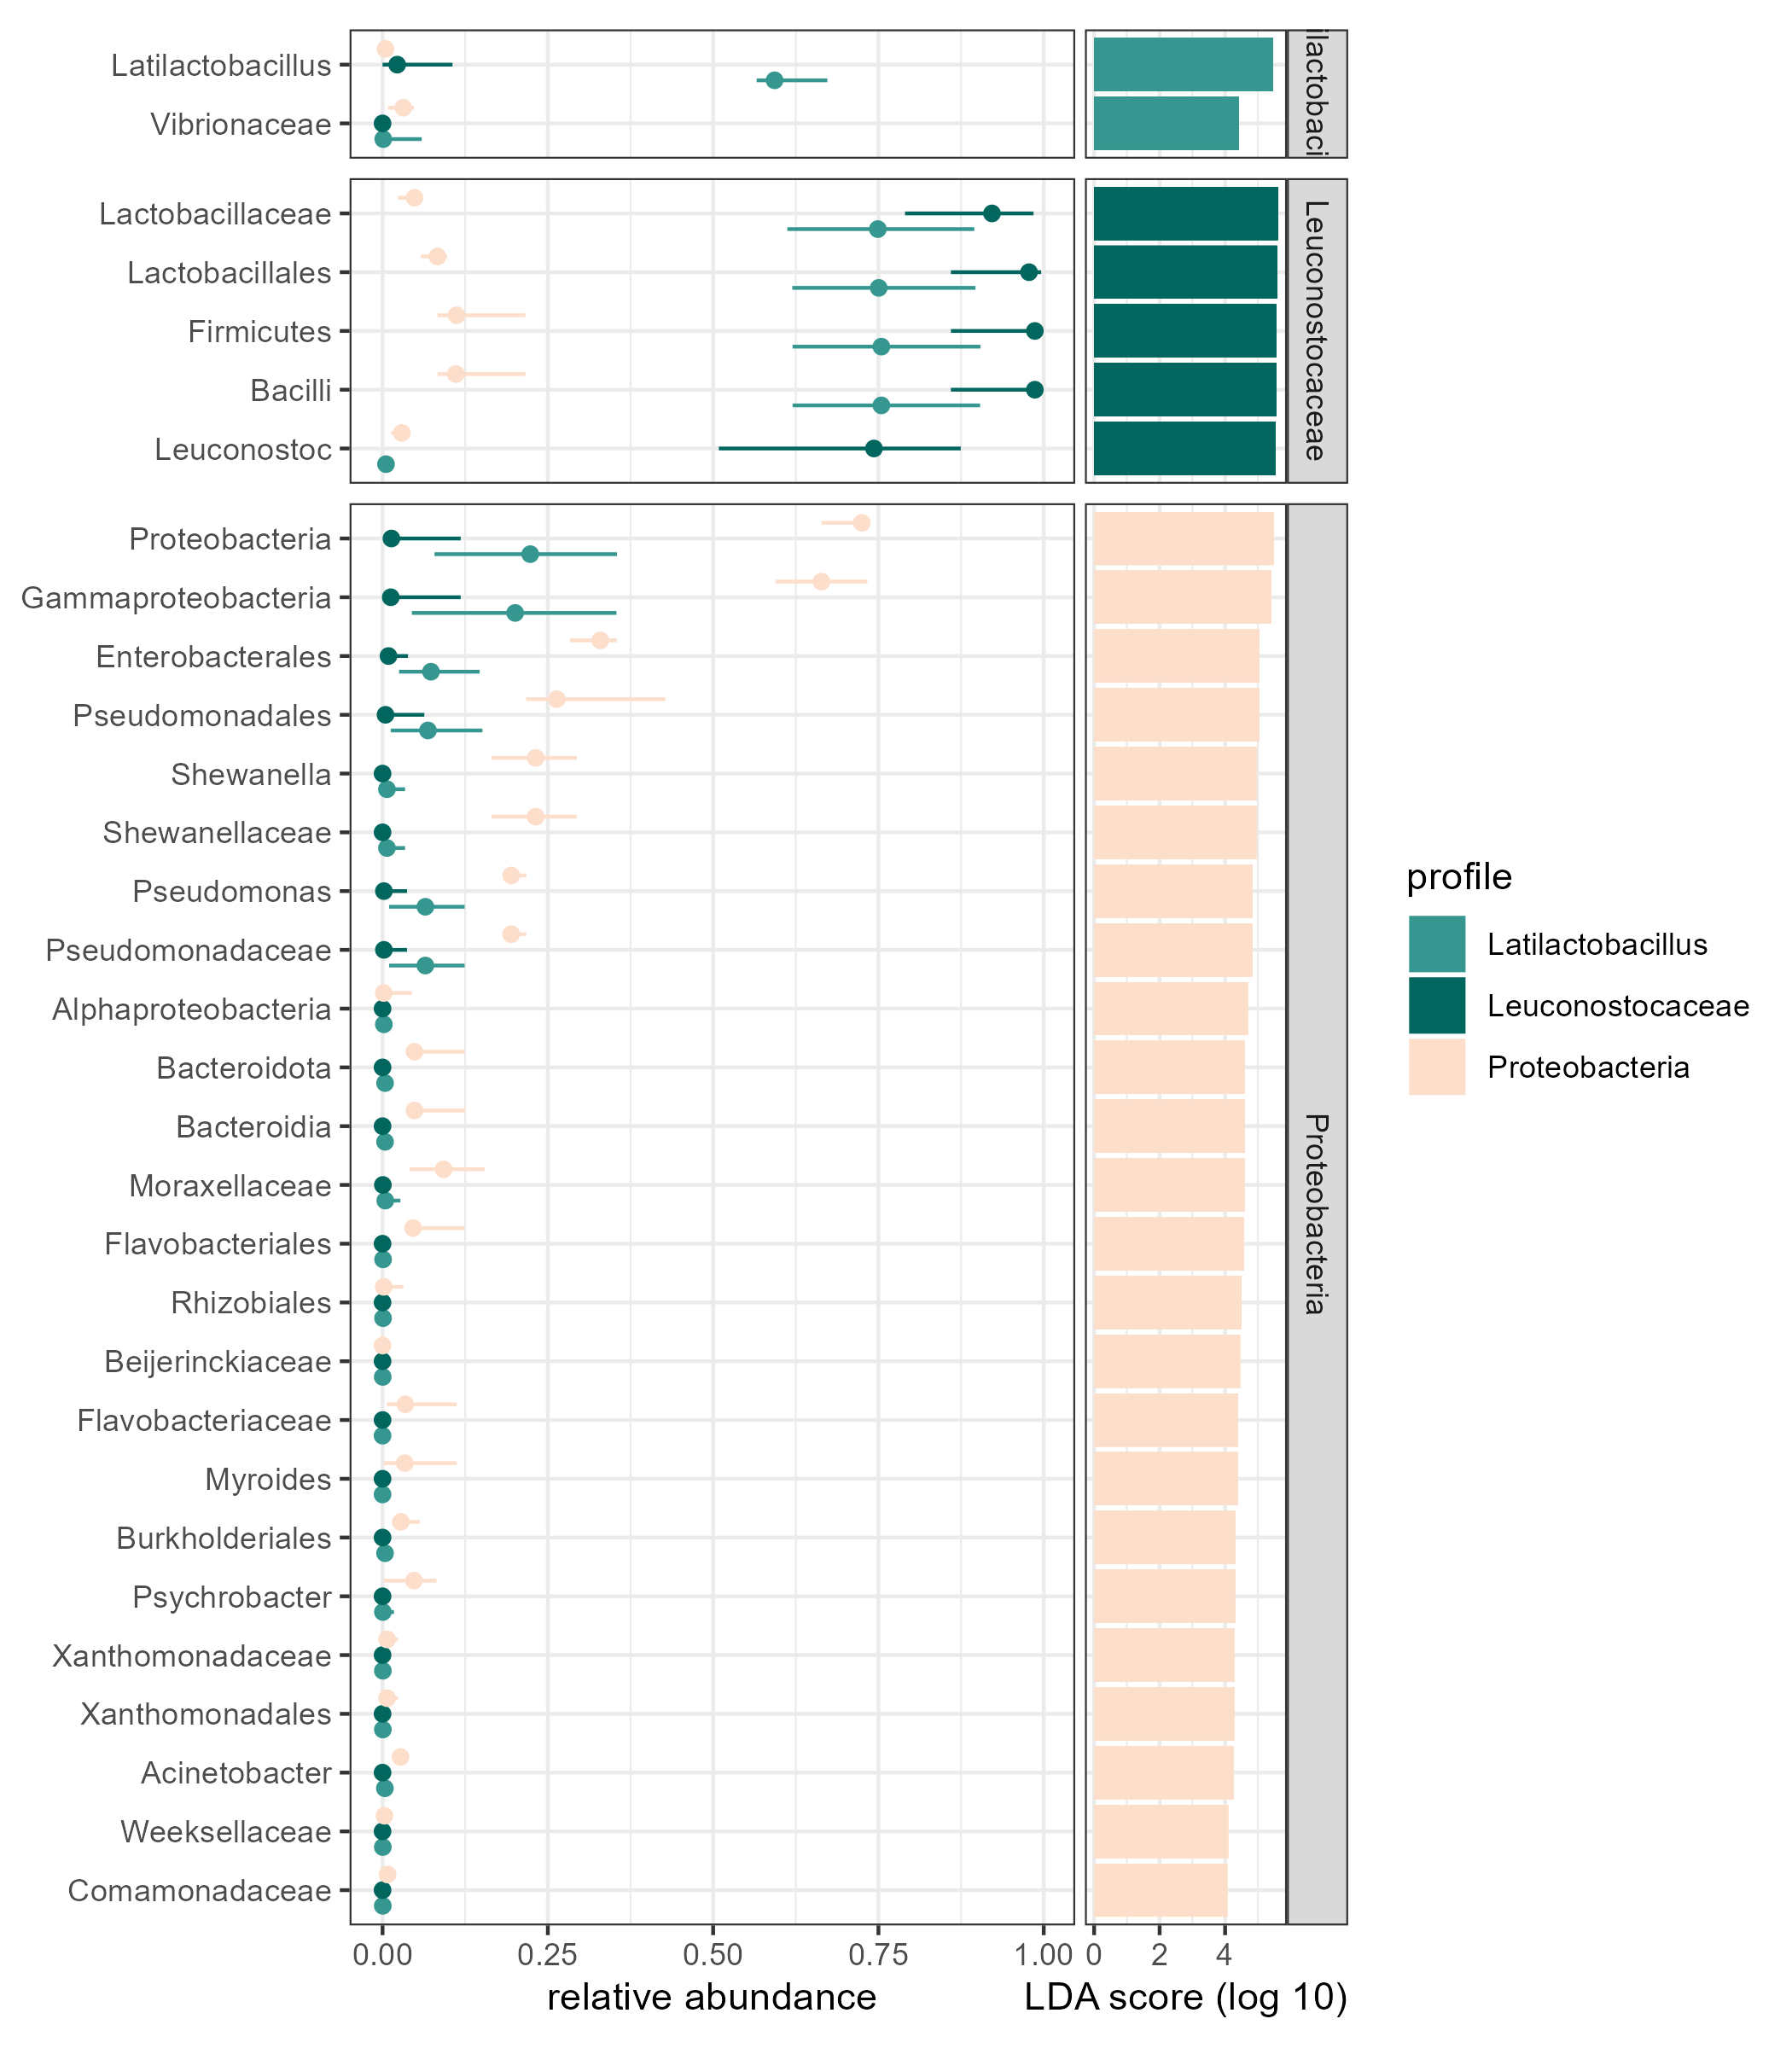
\includegraphics[width=1\linewidth]{lefsestatplot_profile} 

}

\caption{\label{figSM5} LEfSe per profile.  }\label{fig:figSM5}
\end{figure}

s 1 - alpha div group s 2 - NMDS s 3 - PERMANOVA res s 4 - LEfSE group s
5 - LEfSe profile

\newpage

\hypertarget{references}{%
\section*{References}\label{references}}
\addcontentsline{toc}{section}{References}

\hypertarget{refs}{}
\begin{CSLReferences}{0}{0}
\leavevmode\vadjust pre{\hypertarget{ref-EuropeanCommission.2020}{}}%
\CSLLeftMargin{{[}1{]} }%
\CSLRightInline{European Commission, Directorate-General for Agriculture
and Rural Development, EU agricultural outlook for markets and income
2019-2030, {Publications Office}, 2020.
https://doi.org/\href{https://doi.org/10.2762/904294}{10.2762/904294}.}

\leavevmode\vadjust pre{\hypertarget{ref-OECD.2022}{}}%
\CSLLeftMargin{{[}2{]} }%
\CSLRightInline{OECD, Meat consumption (indicator)., OECD, 2022.
https://doi.org/\href{https://doi.org/10.1787/fa290fd0-en}{10.1787/fa290fd0-en}.}

\leavevmode\vadjust pre{\hypertarget{ref-OECDandFoodandAgricultureOrganizationoftheUnitedNations.2022}{}}%
\CSLLeftMargin{{[}3{]} }%
\CSLRightInline{OECD and Food and Agriculture Organization of the United
Nations, OECD-FAO agricultural outlook 2022-2031, OECD, 2022.
https://doi.org/\href{https://doi.org/10.1787/f1b0b29c-en}{10.1787/f1b0b29c-en}.}

\leavevmode\vadjust pre{\hypertarget{ref-Steinfeld.2006}{}}%
\CSLLeftMargin{{[}4{]} }%
\CSLRightInline{H. Steinfeld, Livestock's long shadow: Environmental
issues and options, FAO; {Food and Agriculture Organization of the
United Nations}, Rom, 2006.}

\leavevmode\vadjust pre{\hypertarget{ref-Bianchi.2018}{}}%
\CSLLeftMargin{{[}5{]} }%
\CSLRightInline{F. Bianchi, E. Garnett, C. Dorsel, P. Aveyard, S.A.
Jebb, Restructuring physical micro-environments to reduce the demand for
meat: A systematic review and qualitative comparative analysis, The
Lancet Planetary Health. 2 (2018) e384--e397.
https://doi.org/\href{https://doi.org/10.1016/S2542-5196(18)30188-8}{10.1016/S2542-5196(18)30188-8}.}

\leavevmode\vadjust pre{\hypertarget{ref-Economou.2015}{}}%
\CSLLeftMargin{{[}6{]} }%
\CSLRightInline{V. Economou, P. Gousia, Agriculture and food animals as
a source of antimicrobial-resistant bacteria, Infection and Drug
Resistance. 8 (2015) 49--61.
https://doi.org/\href{https://doi.org/10.2147/IDR.S55778}{10.2147/IDR.S55778}.}

\leavevmode\vadjust pre{\hypertarget{ref-Watts.2018}{}}%
\CSLLeftMargin{{[}7{]} }%
\CSLRightInline{N. Watts, M. Amann, S. Ayeb-Karlsson, K. Belesova, T.
Bouley, M. Boykoff, P. Byass, W. Cai, D. Campbell-Lendrum, J. Chambers,
P.M. Cox, M. Daly, N. Dasandi, M. Davies, M. Depledge, A. Depoux, P.
Dominguez-Salas, P. Drummond, P. Ekins, A. Flahault, H. Frumkin, L.
Georgeson, M. Ghanei, D. Grace, H. Graham, R. Grojsman, A. Haines, I.
Hamilton, S. Hartinger, A. Johnson, I. Kelman, G. Kiesewetter, D.
Kniveton, L. Liang, M. Lott, R. Lowe, G. Mace, M. Odhiambo Sewe, M.
Maslin, S. Mikhaylov, J. Milner, A.M. Latifi, M. Moradi-Lakeh, K.
Morrissey, K. Murray, T. Neville, M. Nilsson, T. Oreszczyn, F. Owfi, D.
Pencheon, S. Pye, M. Rabbaniha, E. Robinson, J. Rocklöv, S. Schütte, J.
Shumake-Guillemot, R. Steinbach, M. Tabatabaei, N. Wheeler, P.
Wilkinson, P. Gong, H. Montgomery, A. Costello, The lancet countdown on
health and climate change: From 25 years of inaction to a global
transformation for public health, The Lancet. 391 (2018) 581--630.
https://doi.org/\href{https://doi.org/10.1016/s0140-6736(17)32464-9}{10.1016/s0140-6736(17)32464-9}.}

\leavevmode\vadjust pre{\hypertarget{ref-Micha.2010}{}}%
\CSLLeftMargin{{[}8{]} }%
\CSLRightInline{R. Micha, S.K. Wallace, D. Mozaffarian, Red and
processed meat consumption and risk of incident coronary heart disease,
stroke, and diabetes mellitus: A systematic review and meta-analysis,
Circulation. 121 (2010) 2271--2283.
https://doi.org/\href{https://doi.org/10.1161/CIRCULATIONAHA.109.924977}{10.1161/CIRCULATIONAHA.109.924977}.}

\leavevmode\vadjust pre{\hypertarget{ref-Chan.2011}{}}%
\CSLLeftMargin{{[}9{]} }%
\CSLRightInline{D.S.M. Chan, R. Lau, D. Aune, R. Vieira, D.C. Greenwood,
E. Kampman, T. Norat, Red and processed meat and colorectal cancer
incidence: Meta-analysis of prospective studies, PloS One. 6 (2011)
e20456.
https://doi.org/\href{https://doi.org/10.1371/journal.pone.0020456}{10.1371/journal.pone.0020456}.}

\leavevmode\vadjust pre{\hypertarget{ref-Parkin.2011}{}}%
\CSLLeftMargin{{[}10{]} }%
\CSLRightInline{D.M. Parkin, L. Boyd, L.C. Walker, 16. The fraction of
cancer attributable to lifestyle and environmental factors in the UK in
2010, British Journal of Cancer. 105 Suppl 2 (2011) S77--81.
https://doi.org/\href{https://doi.org/10.1038/bjc.2011.489}{10.1038/bjc.2011.489}.}

\leavevmode\vadjust pre{\hypertarget{ref-Feskens.2013}{}}%
\CSLLeftMargin{{[}11{]} }%
\CSLRightInline{E.J.M. Feskens, D. Sluik, G.J. van Woudenbergh, Meat
consumption, diabetes, and its complications, Current Diabetes Reports.
13 (2013) 298--306.
https://doi.org/\href{https://doi.org/10.1007/s11892-013-0365-0}{10.1007/s11892-013-0365-0}.}

\leavevmode\vadjust pre{\hypertarget{ref-StollKleemann.2017}{}}%
\CSLLeftMargin{{[}12{]} }%
\CSLRightInline{S. Stoll-Kleemann, U.J. Schmidt, Reducing meat
consumption in developed and transition countries to counter climate
change and biodiversity loss: A review of influence factors, Regional
Environmental Change. 17 (2017) 1261--1277.
https://doi.org/\href{https://doi.org/10.1007/s10113-016-1057-5}{10.1007/s10113-016-1057-5}.}

\leavevmode\vadjust pre{\hypertarget{ref-Ploll.2020}{}}%
\CSLLeftMargin{{[}13{]} }%
\CSLRightInline{U. Ploll, T. Stern, From diet to behaviour: Exploring
environmental- and animal-conscious behaviour among austrian vegetarians
and vegans, British Food Journal. 122 (2020) 3249--3265.
https://doi.org/\href{https://doi.org/10.1108/BFJ-06-2019-0418}{10.1108/BFJ-06-2019-0418}.}

\leavevmode\vadjust pre{\hypertarget{ref-EuropeanUnionsHorizon2020reasearchandinnovationprogramme.2021b}{}}%
\CSLLeftMargin{{[}14{]} }%
\CSLRightInline{European Union's Horizon 2020 reasearch and innovation
programme, Plant-based foods in europe: How big is the market? Smart
protein plant-based food sector report, (2021).
\url{https://smartproteinproject.eu/plant-based-food-sector-report}.}

\leavevmode\vadjust pre{\hypertarget{ref-Neuhofer.2022}{}}%
\CSLLeftMargin{{[}15{]} }%
\CSLRightInline{Z.T. Neuhofer, J.L. Lusk, Most plant-based meat
alternative buyers also buy meat: An analysis of household demographics,
habit formation, and buying behavior among meat alternative buyers,
Scientific Reports. 12 (2022) 13062.
https://doi.org/\href{https://doi.org/10.1038/s41598-022-16996-5}{10.1038/s41598-022-16996-5}.}

\leavevmode\vadjust pre{\hypertarget{ref-EuropeanUnionsHorizon2020reasearchandinnovationprogramme.2021}{}}%
\CSLLeftMargin{{[}16{]} }%
\CSLRightInline{European Union's Horizon 2020 reasearch and innovation
programme, What consumers want: A survey on european consumer attitudes
towards plant-based foods, with a focus on flexitarians: European
union's horizon 2020 research and innovation programme (no 862957),
(2021).
\href{https://www.smartproteinproject.eu/consumer-attitudes-plant-based-food-report}{www.smartproteinproject.eu/consumer-attitudes-plant-based-food-report}
(accessed December 7, 2021).}

\leavevmode\vadjust pre{\hypertarget{ref-Curtain.2019}{}}%
\CSLLeftMargin{{[}17{]} }%
\CSLRightInline{F. Curtain, S. Grafenauer, Plant-based meat substitutes
in the flexitarian age: An audit of products on supermarket shelves,
Nutrients. 11 (2019).
https://doi.org/\href{https://doi.org/10.3390/nu11112603}{10.3390/nu11112603}.}

\leavevmode\vadjust pre{\hypertarget{ref-Crowe.1973}{}}%
\CSLLeftMargin{{[}18{]} }%
\CSLRightInline{C.C. Crowe, W.E. Sanders, S. Longley, Bacterial
interference. II. Role of the normal throat flora in prevention of
colonization by group a streptococcus, The Journal of Infectious
Diseases. 128 (1973) 527--532.
https://doi.org/\href{https://doi.org/10.1093/infdis/128.4.527}{10.1093/infdis/128.4.527}.}

\leavevmode\vadjust pre{\hypertarget{ref-Mackowiak.1982}{}}%
\CSLLeftMargin{{[}19{]} }%
\CSLRightInline{P.A. Mackowiak, The normal microbial flora, The New
England Journal of Medicine. 307 (1982) 83--93.
https://doi.org/\href{https://doi.org/10.1056/nejm198207083070203}{10.1056/nejm198207083070203}.}

\leavevmode\vadjust pre{\hypertarget{ref-Smith.2007}{}}%
\CSLLeftMargin{{[}20{]} }%
\CSLRightInline{K. Smith, K.D. McCoy, A.J. Macpherson, Use of axenic
animals in studying the adaptation of mammals to their commensal
intestinal microbiota, Seminars in Immunology. 19 (2007) 59--69.
https://doi.org/\href{https://doi.org/10.1016/j.smim.2006.10.002}{10.1016/j.smim.2006.10.002}.}

\leavevmode\vadjust pre{\hypertarget{ref-Blaser.2009}{}}%
\CSLLeftMargin{{[}21{]} }%
\CSLRightInline{M.J. Blaser, S. Falkow, What are the consequences of the
disappearing human microbiota?, Nature Reviews. Microbiology. 7 (2009)
887--894.
https://doi.org/\href{https://doi.org/10.1038/nrmicro2245}{10.1038/nrmicro2245}.}

\leavevmode\vadjust pre{\hypertarget{ref-Vangay.2018}{}}%
\CSLLeftMargin{{[}22{]} }%
\CSLRightInline{P. Vangay, A.J. Johnson, T.L. Ward, G.A. Al-Ghalith,
R.R. Shields-Cutler, B.M. Hillmann, S.K. Lucas, L.K. Beura, E.A.
Thompson, L.M. Till, R. Batres, B. Paw, S.L. Pergament, P. Saenyakul, M.
Xiong, A.D. Kim, G. Kim, D. Masopust, E.C. Martens, C. Angkurawaranon,
R. McGready, P.C. Kashyap, K.A. Culhane-Pera, D. Knights, US immigration
westernizes the human gut microbiome, Cell. 175 (2018) 962--972.e10.
https://doi.org/\href{https://doi.org/10.1016/j.cell.2018.10.029}{10.1016/j.cell.2018.10.029}.}

\leavevmode\vadjust pre{\hypertarget{ref-Walsh.2013}{}}%
\CSLLeftMargin{{[}23{]} }%
\CSLRightInline{P.S. Walsh, D.A. Metzger, R. Higushi, Chelex 100 as a
medium for simple extraction of DNA for PCR-based typing from forensic
material. BioTechniques 10(4): 506-13 (april 1991), BioTechniques. 54
(2013) 134--139.
https://doi.org/\href{https://doi.org/10.2144/000114018}{10.2144/000114018}.}

\leavevmode\vadjust pre{\hypertarget{ref-OxfordNanoporeTechnologies.2021}{}}%
\CSLLeftMargin{{[}24{]} }%
\CSLRightInline{Oxford Nanopore Technologies, Ligation sequencing gDNA -
native barcoding (SQK-LSK109 with EXP-NBD196): Version:
NBE{\_}9121{\_}v109{\_}revE{\_}19Jan2021, (2021).}

\leavevmode\vadjust pre{\hypertarget{ref-Qiagen.2017}{}}%
\CSLLeftMargin{{[}25{]} }%
\CSLRightInline{Qiagen, DNeasy PowerFood microbial kit handbook 10/2017:
HB-2271-001, (2017).}

\leavevmode\vadjust pre{\hypertarget{ref-Bolyen.2019}{}}%
\CSLLeftMargin{{[}26{]} }%
\CSLRightInline{E. Bolyen, J.R. Rideout, M.R. Dillon, N.A. Bokulich,
C.C. Abnet, G.A. Al-Ghalith, H. Alexander, E.J. Alm, M. Arumugam, F.
Asnicar, Y. Bai, J.E. Bisanz, K. Bittinger, A. Brejnrod, C.J. Brislawn,
C.T. Brown, B.J. Callahan, A.M. Caraballo-Rodríguez, J. Chase, E.K.
Cope, R. Da Silva, C. Diener, P.C. Dorrestein, G.M. Douglas, D.M.
Durall, C. Duvallet, C.F. Edwardson, M. Ernst, M. Estaki, J. Fouquier,
J.M. Gauglitz, S.M. Gibbons, D.L. Gibson, A. Gonzalez, K. Gorlick, J.
Guo, B. Hillmann, S. Holmes, H. Holste, C. Huttenhower, G.A. Huttley, S.
Janssen, A.K. Jarmusch, L. Jiang, B.D. Kaehler, K.B. Kang, C.R. Keefe,
P. Keim, S.T. Kelley, D. Knights, I. Koester, T. Kosciolek, J. Kreps,
M.G.I. Langille, J. Lee, R. Ley, Y.-X. Liu, E. Loftfield, C. Lozupone,
M. Maher, C. Marotz, B.D. Martin, D. McDonald, L.J. McIver, A.V. Melnik,
J.L. Metcalf, S.C. Morgan, J.T. Morton, A.T. Naimey, J.A. Navas-Molina,
L.F. Nothias, S.B. Orchanian, T. Pearson, S.L. Peoples, D. Petras, M.L.
Preuss, E. Pruesse, L.B. Rasmussen, A. Rivers, M.S. Robeson, P.
Rosenthal, N. Segata, M. Shaffer, A. Shiffer, R. Sinha, S.J. Song, J.R.
Spear, A.D. Swafford, L.R. Thompson, P.J. Torres, P. Trinh, A. Tripathi,
P.J. Turnbaugh, S. Ul-Hasan, J.J.J. van der Hooft, F. Vargas, Y.
Vázquez-Baeza, E. Vogtmann, M. von Hippel, W. Walters, Y. Wan, M. Wang,
J. Warren, K.C. Weber, C.H.D. Williamson, A.D. Willis, Z.Z. Xu, J.R.
Zaneveld, Y. Zhang, Q. Zhu, R. Knight, J.G. Caporaso, Reproducible,
interactive, scalable and extensible microbiome data science using QIIME
2, Nature Biotechnology. 37 (2019) 852--857.
https://doi.org/\href{https://doi.org/10.1038/s41587-019-0209-9}{10.1038/s41587-019-0209-9}.}

\leavevmode\vadjust pre{\hypertarget{ref-Quast.2013}{}}%
\CSLLeftMargin{{[}27{]} }%
\CSLRightInline{C. Quast, E. Pruesse, P. Yilmaz, J. Gerken, T. Schweer,
P. Yarza, J. Peplies, F.O. Glöckner, The SILVA ribosomal RNA gene
database project: Improved data processing and web-based tools, Nucleic
Acids Research. 41 (2013) D590--6.
https://doi.org/\href{https://doi.org/10.1093/nar/gks1219}{10.1093/nar/gks1219}.}

\leavevmode\vadjust pre{\hypertarget{ref-Bokulich.2018}{}}%
\CSLLeftMargin{{[}28{]} }%
\CSLRightInline{N.A. Bokulich, B.D. Kaehler, J.R. Rideout, M. Dillon, E.
Bolyen, R. Knight, G.A. Huttley, J. Gregory Caporaso, Optimizing
taxonomic classification of marker-gene amplicon sequences with QIIME
2's q2-feature-classifier plugin, Microbiome. 6 (2018) 90.
https://doi.org/\href{https://doi.org/10.1186/s40168-018-0470-z}{10.1186/s40168-018-0470-z}.}

\leavevmode\vadjust pre{\hypertarget{ref-Kaehler.2019}{}}%
\CSLLeftMargin{{[}29{]} }%
\CSLRightInline{B.D. Kaehler, N.A. Bokulich, D. McDonald, R. Knight,
J.G. Caporaso, G.A. Huttley, Species abundance information improves
sequence taxonomy classification accuracy, Nature Communications. 10
(2019) 4643.
https://doi.org/\href{https://doi.org/10.1038/s41467-019-12669-6}{10.1038/s41467-019-12669-6}.}

\leavevmode\vadjust pre{\hypertarget{ref-Robeson.2021}{}}%
\CSLLeftMargin{{[}30{]} }%
\CSLRightInline{M.S. Robeson, D.R. O'Rourke, B.D. Kaehler, M. Ziemski,
M.R. Dillon, J.T. Foster, N.A. Bokulich, RESCRIPt: Reproducible sequence
taxonomy reference database management, PLoS Computational Biology. 17
(2021) e1009581.
https://doi.org/\href{https://doi.org/10.1371/journal.pcbi.1009581}{10.1371/journal.pcbi.1009581}.}

\leavevmode\vadjust pre{\hypertarget{ref-Kaehler.2022}{}}%
\CSLLeftMargin{{[}31{]} }%
\CSLRightInline{B.D. Kaehler, Silva 138.1 taxonomy classifiers for use
with QIIME 2 q2-feature-classifier, (2022).
https://doi.org/\href{https://doi.org/10.5281/zenodo.6395539}{10.5281/zenodo.6395539}.}

\leavevmode\vadjust pre{\hypertarget{ref-RCoreTeam.2021}{}}%
\CSLLeftMargin{{[}32{]} }%
\CSLRightInline{R Core Team, R: A language and environment for
statistical computing, (2021). \url{https://www.R-project.org/}.}

\leavevmode\vadjust pre{\hypertarget{ref-Hsieh.2022}{}}%
\CSLLeftMargin{{[}33{]} }%
\CSLRightInline{T.C. Hsieh, K.H. Ma, A. Chao, iNEXT: Interpolation and
extrapolation for species diversity, (2022).
\url{http://chao.stat.nthu.edu.tw/wordpress/software_download/}.}

\leavevmode\vadjust pre{\hypertarget{ref-Chao.2012}{}}%
\CSLLeftMargin{{[}34{]} }%
\CSLRightInline{A. Chao, L. Jost, Coverage-based rarefaction and
extrapolation: Standardizing samples by completeness rather than size,
Ecology. 93 (2012) 2533--2547.
https://doi.org/\href{https://doi.org/10.1890/11-1952.1}{10.1890/11-1952.1}.}

\leavevmode\vadjust pre{\hypertarget{ref-Roswell.2021}{}}%
\CSLLeftMargin{{[}35{]} }%
\CSLRightInline{M. Roswell, J. Dushoff, R. Winfree, A conceptual guide
to measuring species diversity, Oikos. 130 (2021) 321--338.
https://doi.org/\href{https://doi.org/10.1111/oik.07202}{10.1111/oik.07202}.}

\leavevmode\vadjust pre{\hypertarget{ref-McMurdie.2021}{}}%
\CSLLeftMargin{{[}36{]} }%
\CSLRightInline{P.J. McMurdie, S. Holmes, with contributions from
Gregory Jordan, S. Chamberlain, Phyloseq: Handling and analysis of
high-throughput microbiome census data, (2021).
\url{http://dx.plos.org/10.1371/journal.pone.0061217}.}

\leavevmode\vadjust pre{\hypertarget{ref-Mikryukov.2022}{}}%
\CSLLeftMargin{{[}37{]} }%
\CSLRightInline{V. Mikryukov, metagMisc: Miscellaneous functions for
metagenomic analysis, (2022).}

\leavevmode\vadjust pre{\hypertarget{ref-Krijthe.2022}{}}%
\CSLLeftMargin{{[}38{]} }%
\CSLRightInline{J. Krijthe, Rtsne: T-distributed stochastic neighbor
embedding using a barnes-hut implementation, (2022).
\url{https://github.com/jkrijthe/Rtsne}.}

\leavevmode\vadjust pre{\hypertarget{ref-Oskolkov.2019}{}}%
\CSLLeftMargin{{[}39{]} }%
\CSLRightInline{N. Oskolkov, How to tune hyperparameters of tSNE: Three
simple rules to make beautiful tSNE plots, (2019).
\url{https://towardsdatascience.com/how-to-tune-hyperparameters-of-tsne-7c0596a18868\#:~:text=The\%20optimal\%20perplexity\%20can\%20be\%20calculated\%20from\%20the\%20number\%20of,data\%20points\%20of\%20~100\%20units.}}

\leavevmode\vadjust pre{\hypertarget{ref-Oksanen.2022}{}}%
\CSLLeftMargin{{[}40{]} }%
\CSLRightInline{J. Oksanen, G.L. Simpson, F.G. Blanchet, R. Kindt, P.
Legendre, P.R. Minchin, R.B. O'Hara, P. Solymos, M.H.H. Stevens, E.
Szoecs, H. Wagner, M. Barbour, M. Bedward, B. Bolker, D. Borcard, G.
Carvalho, M. Chirico, M.D. Caceres, S. Durand, H.B.A. Evangelista, R.
FitzJohn, M. Friendly, B. Furneaux, G. Hannigan, M.O. Hill, L. Lahti, D.
McGlinn, M.-H. Ouellette, E.R. Cunha, T. Smith, A. Stier, C.J.F.T.
Braak, J. Weedon, Vegan: Community ecology package, (2022).
\url{https://github.com/vegandevs/vegan}.}

\leavevmode\vadjust pre{\hypertarget{ref-Stagaman.2022}{}}%
\CSLLeftMargin{{[}41{]} }%
\CSLRightInline{K. Stagaman, phyloseqCompanion: Provides additional
functions to work with phyloseq objects, (2022).}

\leavevmode\vadjust pre{\hypertarget{ref-Segata.2011}{}}%
\CSLLeftMargin{{[}42{]} }%
\CSLRightInline{N. Segata, J. Izard, L. Waldron, D. Gevers, L.
Miropolsky, W.S. Garrett, C. Huttenhower, Metagenomic biomarker
discovery and explanation, Genome Biology. 12 (2011) R60.
https://doi.org/\href{https://doi.org/10.1186/gb-2011-12-6-r60}{10.1186/gb-2011-12-6-r60}.}

\leavevmode\vadjust pre{\hypertarget{ref-Chao.2020}{}}%
\CSLLeftMargin{{[}43{]} }%
\CSLRightInline{K.-H. Chao, K. Barton, S. Palmer, R. Lanfear,
sangeranalyseR: Simple and interactive analysis of sanger sequencing
data in r, bioRxiv. (2020).
https://doi.org/\href{https://doi.org/10.1101/2020.05.18.102459}{10.1101/2020.05.18.102459}.}

\leavevmode\vadjust pre{\hypertarget{ref-Callahan.2016}{}}%
\CSLLeftMargin{{[}44{]} }%
\CSLRightInline{B.J. Callahan, P.J. McMurdie, M.J. Rosen, A.W. Han,
A.J.A. Johnson, S.P. Holmes, DADA2: High-resolution sample inference
from illumina amplicon data, Nature Methods. 13 (2016) 581--583.
https://doi.org/\href{https://doi.org/10.1038/nmeth.3869}{10.1038/nmeth.3869}.}

\leavevmode\vadjust pre{\hypertarget{ref-Wright.2016}{}}%
\CSLLeftMargin{{[}45{]} }%
\CSLRightInline{E.S. Wright, Using DECIPHER v2.0 to analyze big
biological sequence data in r, The R Journal. 8 (2016) 352--359.}

\leavevmode\vadjust pre{\hypertarget{ref-Wick.2021}{}}%
\CSLLeftMargin{{[}46{]} }%
\CSLRightInline{R. Wick, Filtlong, (2021).
\url{https://github.com/rrwick/Filtlong}.}

\leavevmode\vadjust pre{\hypertarget{ref-Kolmogorov.2019}{}}%
\CSLLeftMargin{{[}47{]} }%
\CSLRightInline{M. Kolmogorov, J. Yuan, Y. Lin, P.A. Pevzner, Assembly
of long, error-prone reads using repeat graphs, Nature Biotechnology. 37
(2019) 540--546.
https://doi.org/\href{https://doi.org/10.1038/s41587-019-0072-8}{10.1038/s41587-019-0072-8}.}

\leavevmode\vadjust pre{\hypertarget{ref-Lin.2016}{}}%
\CSLLeftMargin{{[}48{]} }%
\CSLRightInline{Y. Lin, J. Yuan, M. Kolmogorov, M.W. Shen, M. Chaisson,
P.A. Pevzner, Assembly of long error-prone reads using de bruijn graphs,
Proceedings of the National Academy of Sciences of the United States of
America. 113 (2016) E8396--E8405.
https://doi.org/\href{https://doi.org/10.1073/pnas.1604560113}{10.1073/pnas.1604560113}.}

\leavevmode\vadjust pre{\hypertarget{ref-Vaser.2017}{}}%
\CSLLeftMargin{{[}49{]} }%
\CSLRightInline{R. Vaser, I. Sović, N. Nagarajan, M. Šikić, Fast and
accurate de novo genome assembly from long uncorrected reads, Genome
Research. 27 (2017) 737--746.
https://doi.org/\href{https://doi.org/10.1101/gr.214270.116}{10.1101/gr.214270.116}.}

\leavevmode\vadjust pre{\hypertarget{ref-OxfordNanoporeTechnologies.2022}{}}%
\CSLLeftMargin{{[}50{]} }%
\CSLRightInline{Oxford Nanopore Technologies, (2022).
\url{https://github.com/nanoporetech/medaka}.}

\leavevmode\vadjust pre{\hypertarget{ref-Quijada.2019}{}}%
\CSLLeftMargin{{[}51{]} }%
\CSLRightInline{N.M. Quijada, D. Rodríguez-Lázaro, J.M. Eiros, M.
Hernández, TORMES: An automated pipeline for whole bacterial genome
analysis, Bioinformatics (Oxford, England). 35 (2019) 4207--4212.
https://doi.org/\href{https://doi.org/10.1093/bioinformatics/btz220}{10.1093/bioinformatics/btz220}.}

\leavevmode\vadjust pre{\hypertarget{ref-Prjibelski.2020}{}}%
\CSLLeftMargin{{[}52{]} }%
\CSLRightInline{A. Prjibelski, D. Antipov, D. Meleshko, A. Lapidus, A.
Korobeynikov, Using SPAdes de novo assembler, Current Protocols in
Bioinformatics. 70 (2020) e102.
https://doi.org/\href{https://doi.org/10.1002/cpbi.102}{10.1002/cpbi.102}.}

\leavevmode\vadjust pre{\hypertarget{ref-Hyatt.2016}{}}%
\CSLLeftMargin{{[}53{]} }%
\CSLRightInline{D. Hyatt, Prodigal, GitHub Repository. (2016).}

\leavevmode\vadjust pre{\hypertarget{ref-Seemann.2014}{}}%
\CSLLeftMargin{{[}54{]} }%
\CSLRightInline{T. Seemann, Prokka: Rapid prokaryotic genome annotation,
Bioinformatics (Oxford, England). 30 (2014) 2068--2069.
https://doi.org/\href{https://doi.org/10.1093/bioinformatics/btu153}{10.1093/bioinformatics/btu153}.}

\leavevmode\vadjust pre{\hypertarget{ref-Seemann.2020}{}}%
\CSLLeftMargin{{[}55{]} }%
\CSLRightInline{T. Seemann, Abricate, GitHub Repository. (2020).}

\leavevmode\vadjust pre{\hypertarget{ref-McArthur.2013}{}}%
\CSLLeftMargin{{[}56{]} }%
\CSLRightInline{A.G. McArthur, N. Waglechner, F. Nizam, A. Yan, M.A.
Azad, A.J. Baylay, K. Bhullar, M.J. Canova, G. de Pascale, L. Ejim, L.
Kalan, A.M. King, K. Koteva, M. Morar, M.R. Mulvey, J.S. O'Brien, A.C.
Pawlowski, L.J.V. Piddock, P. Spanogiannopoulos, A.D. Sutherland, I.
Tang, P.L. Taylor, M. Thaker, W. Wang, M. Yan, T. Yu, G.D. Wright, The
comprehensive antibiotic resistance database, Antimicrobial Agents and
Chemotherapy. 57 (2013) 3348--3357.
https://doi.org/\href{https://doi.org/10.1128/AAC.00419-13}{10.1128/AAC.00419-13}.}

\leavevmode\vadjust pre{\hypertarget{ref-Chen.2005}{}}%
\CSLLeftMargin{{[}57{]} }%
\CSLRightInline{L. Chen, J. Yang, J. Yu, Z. Yao, L. Sun, Y. Shen, Q.
Jin, VFDB: A reference database for bacterial virulence factors, Nucleic
Acids Research. 33 (2005) D325--8.
https://doi.org/\href{https://doi.org/10.1093/nar/gki008}{10.1093/nar/gki008}.}

\leavevmode\vadjust pre{\hypertarget{ref-Chaumeil.2022}{}}%
\CSLLeftMargin{{[}58{]} }%
\CSLRightInline{P.-A. Chaumeil, A.J. Mussig, P. Hugenholtz, D.H. Parks,
GTDB-tk v2: Memory friendly classification with the genome taxonomy
database, Bioinformatics (Oxford, England). 38 (2022) 5315--5316.
https://doi.org/\href{https://doi.org/10.1093/bioinformatics/btac672}{10.1093/bioinformatics/btac672}.}

\leavevmode\vadjust pre{\hypertarget{ref-Parks.2022}{}}%
\CSLLeftMargin{{[}59{]} }%
\CSLRightInline{D.H. Parks, M. Chuvochina, C. Rinke, A.J. Mussig, P.-A.
Chaumeil, P. Hugenholtz, GTDB: An ongoing census of bacterial and
archaeal diversity through a phylogenetically consistent, rank
normalized and complete genome-based taxonomy, Nucleic Acids Research.
50 (2022) D785--D794.
https://doi.org/\href{https://doi.org/10.1093/nar/gkab776}{10.1093/nar/gkab776}.}

\leavevmode\vadjust pre{\hypertarget{ref-Jolley.2018}{}}%
\CSLLeftMargin{{[}60{]} }%
\CSLRightInline{K.A. Jolley, J.E. Bray, M.C.J. Maiden, Open-access
bacterial population genomics: BIGSdb software, the PubMLST.org website
and their applications, Wellcome Open Research. 3 (2018) 124.
https://doi.org/\href{https://doi.org/10.12688/wellcomeopenres.14826.1}{10.12688/wellcomeopenres.14826.1}.}

\leavevmode\vadjust pre{\hypertarget{ref-Carroll.2020}{}}%
\CSLLeftMargin{{[}61{]} }%
\CSLRightInline{L.M. Carroll, R.A. Cheng, J. Kovac, No assembly
required: Using BTyper3 to assess the congruency of a proposed taxonomic
framework for the bacillus cereus group with historical typing methods,
Frontiers in Microbiology. 11 (2020) 580691.
https://doi.org/\href{https://doi.org/10.3389/fmicb.2020.580691}{10.3389/fmicb.2020.580691}.}

\leavevmode\vadjust pre{\hypertarget{ref-Kanehisa.2016}{}}%
\CSLLeftMargin{{[}62{]} }%
\CSLRightInline{M. Kanehisa, Y. Sato, K. Morishima, BlastKOALA and
GhostKOALA: KEGG tools for functional characterization of genome and
metagenome sequences, Journal of Molecular Biology. 428 (2016) 726--731.
https://doi.org/\href{https://doi.org/10.1016/j.jmb.2015.11.006}{10.1016/j.jmb.2015.11.006}.}

\leavevmode\vadjust pre{\hypertarget{ref-Blin.2021}{}}%
\CSLLeftMargin{{[}63{]} }%
\CSLRightInline{K. Blin, S. Shaw, A.M. Kloosterman, Z. Charlop-Powers,
G.P. van Wezel, M.H. Medema, T. Weber, antiSMASH 6.0: Improving cluster
detection and comparison capabilities, Nucleic Acids Research. 49 (2021)
W29--W35.
https://doi.org/\href{https://doi.org/10.1093/nar/gkab335}{10.1093/nar/gkab335}.}

\leavevmode\vadjust pre{\hypertarget{ref-Bartlett.2022}{}}%
\CSLLeftMargin{{[}64{]} }%
\CSLRightInline{A. Bartlett, D. Padfield, L. Lear, R. Bendall, M. Vos, A
comprehensive list of bacterial pathogens infecting humans,
Microbiology. 168 (2022).
https://doi.org/\href{https://doi.org/10.1099/mic.0.001269}{10.1099/mic.0.001269}.}

\leavevmode\vadjust pre{\hypertarget{ref-Pakbin.2021}{}}%
\CSLLeftMargin{{[}65{]} }%
\CSLRightInline{B. Pakbin, W.M. Brück, J.W.A. Rossen, Virulence factors
of enteric pathogenic escherichia coli: A review, International Journal
of Molecular Sciences. 22 (2021) 9922.
https://doi.org/\href{https://doi.org/10.3390/ijms22189922}{10.3390/ijms22189922}.}

\leavevmode\vadjust pre{\hypertarget{ref-Cosic.2021}{}}%
\CSLLeftMargin{{[}66{]} }%
\CSLRightInline{A. Cosic, E. Leitner, C. Petternel, H. Galler, F.F.
Reinthaler, K.A. Herzog-Obereder, E. Tatscher, S. Raffl, G. Feierl, C.
Högenauer, E.L. Zechner, S. Kienesberger, Variation in accessory genes
within the klebsiella oxytoca species complex delineates monophyletic
members and simplifies coherent genotyping, Frontiers in Microbiology.
12 (2021) 692453.
https://doi.org/\href{https://doi.org/10.3389/fmicb.2021.692453}{10.3389/fmicb.2021.692453}.}

\leavevmode\vadjust pre{\hypertarget{ref-Carroll.2019}{}}%
\CSLLeftMargin{{[}67{]} }%
\CSLRightInline{L.M. Carroll, M. Wiedmann, M. Mukherjee, D.C. Nicholas,
L.A. Mingle, N.B. Dumas, J.A. Cole, J. Kovac, Characterization of emetic
and diarrheal bacillus cereus strains from a 2016 foodborne outbreak
using whole-genome sequencing: Addressing the microbiological,
epidemiological, and bioinformatic challenges, Frontiers in
Microbiology. 10 (2019) 144.
https://doi.org/\href{https://doi.org/10.3389/fmicb.2019.00144}{10.3389/fmicb.2019.00144}.}

\leavevmode\vadjust pre{\hypertarget{ref-Dekkers.2018}{}}%
\CSLLeftMargin{{[}68{]} }%
\CSLRightInline{B.L. Dekkers, R.M. Boom, A.J. van der Goot, Structuring
processes for meat analogues, Trends in Food Science and Technology. 81
(2018) 25--36.
https://doi.org/\href{https://doi.org/10.1016/j.tifs.2018.08.011}{10.1016/j.tifs.2018.08.011}.}

\leavevmode\vadjust pre{\hypertarget{ref-Lin.2002}{}}%
\CSLLeftMargin{{[}69{]} }%
\CSLRightInline{S. Lin, H.E. Huff, F. Hsieh, Extrusion process
parameters, sensory characteristics, and structural properties of a high
moisture soy protein meat analog, Journal of Food Science. 67 (2002)
1066--1072.
https://doi.org/\href{https://doi.org/10.1111/j.1365-2621.2002.tb09454.x}{10.1111/j.1365-2621.2002.tb09454.x}.}

\leavevmode\vadjust pre{\hypertarget{ref-Beniwal.2021}{}}%
\CSLLeftMargin{{[}70{]} }%
\CSLRightInline{A.S. Beniwal, J. Singh, L. Kaur, A. Hardacre, H. Singh,
Meat analogs: Protein restructuring during thermomechanical processing,
Comprehensive Reviews in Food Science and Food Safety. 20 (2021)
1221--1249.
https://doi.org/\href{https://doi.org/10.1111/1541-4337.12721}{10.1111/1541-4337.12721}.}

\leavevmode\vadjust pre{\hypertarget{ref-Ferawati.2021}{}}%
\CSLLeftMargin{{[}71{]} }%
\CSLRightInline{F. Ferawati, I. Zahari, M. Barman, M. Hefni, C.
Ahlström, C. Witthöft, K. Östbring, High-moisture meat analogues
produced from yellow pea and faba bean protein isolates/concentrate:
Effect of raw material composition and extrusion parameters on texture
properties, Foods. 10 (2021).
https://doi.org/\href{https://doi.org/10.3390/foods10040843}{10.3390/foods10040843}.}

\leavevmode\vadjust pre{\hypertarget{ref-Schmid.2022}{}}%
\CSLLeftMargin{{[}72{]} }%
\CSLRightInline{E.-M. Schmid, A. Farahnaky, B. Adhikari, P.J. Torley,
High moisture extrusion cooking of meat analogs: A review of mechanisms
of protein texturization, Comprehensive Reviews in Food Science and Food
Safety. (2022).
https://doi.org/\href{https://doi.org/10.1111/1541-4337.13030}{10.1111/1541-4337.13030}.}

\leavevmode\vadjust pre{\hypertarget{ref-Lin.2000}{}}%
\CSLLeftMargin{{[}73{]} }%
\CSLRightInline{S. Lin, H.E. Huff, F. Hsieh, Texture and chemical
characteristics of soy protein meat analog extruded at high moisture,
Journal of Food Science. 65 (2000) 264--269.
https://doi.org/\href{https://doi.org/10.1111/j.1365-2621.2000.tb15991.x}{10.1111/j.1365-2621.2000.tb15991.x}.}

\leavevmode\vadjust pre{\hypertarget{ref-Guyony.2022}{}}%
\CSLLeftMargin{{[}74{]} }%
\CSLRightInline{V. Guyony, F. Fayolle, V. Jury, High moisture extrusion
of vegetable proteins for making fibrous meat analogs: A review, Food
Reviews International. (2022) 1--26.
https://doi.org/\href{https://doi.org/10.1080/87559129.2021.2023816}{10.1080/87559129.2021.2023816}.}

\leavevmode\vadjust pre{\hypertarget{ref-Kristiawan.2018}{}}%
\CSLLeftMargin{{[}75{]} }%
\CSLRightInline{M. Kristiawan, V. Micard, P. Maladira, C. Alchamieh,
J.-E. Maigret, A.-L. Réguerre, M.A. Emin, G. Della Valle, Multi-scale
structural changes of starch and proteins during pea flour extrusion,
Food Research International (Ottawa, Ont.). 108 (2018) 203--215.
https://doi.org/\href{https://doi.org/10.1016/j.foodres.2018.03.027}{10.1016/j.foodres.2018.03.027}.}

\leavevmode\vadjust pre{\hypertarget{ref-Pietsch.2019}{}}%
\CSLLeftMargin{{[}76{]} }%
\CSLRightInline{V.L. Pietsch, R. Werner, H.P. Karbstein, M.A. Emin, High
moisture extrusion of wheat gluten: Relationship between process
parameters, protein polymerization, and final product characteristics,
Journal of Food Engineering. 259 (2019) 3--11.
https://doi.org/\href{https://doi.org/10.1016/j.jfoodeng.2019.04.006}{10.1016/j.jfoodeng.2019.04.006}.}

\leavevmode\vadjust pre{\hypertarget{ref-Yu.2014}{}}%
\CSLLeftMargin{{[}77{]} }%
\CSLRightInline{L. Yu, Y. Meng, H.S. Ramaswamy, J. Boye, Residence time
distribution of soy protein isolate and corn flour feed mix in a
twin-screw extruder, Journal of Food Processing and Preservation. 38
(2014) 573--584.
https://doi.org/\href{https://doi.org/10.1111/jfpp.12005}{10.1111/jfpp.12005}.}

\leavevmode\vadjust pre{\hypertarget{ref-Mwangi.2008}{}}%
\CSLLeftMargin{{[}78{]} }%
\CSLRightInline{R. Mwangi, Inactivation of wild type bacillus spores in
a soy meat analog model by extrusion cooking, 2008.
https://doi.org/\href{https://doi.org/10.32469/10355\%7B/\%\%7D2F5763}{10.32469/10355\{\textbackslash\%\}2F5763}.}

\leavevmode\vadjust pre{\hypertarget{ref-Leutgeb.2017}{}}%
\CSLLeftMargin{{[}79{]} }%
\CSLRightInline{K. Leutgeb, Microbial examination of raw and extruded
products for production of a vegetarian meat analogue, Masterthesis,
{BOKU-University of natural resources and life sciences, Vienna};
Institute of Food Science, 2017.
\url{https://forschung.boku.ac.at/fis/suchen.person_betreuungen?sprache_in=de\&menue_id_in=107\&id_in=3823}.}

\leavevmode\vadjust pre{\hypertarget{ref-Filho.2005}{}}%
\CSLLeftMargin{{[}80{]} }%
\CSLRightInline{G.C.S. Filho, R.C. Vessoni Penna, D.W. Schaffner,
Microbiological quality of vegetable proteins during the preparation of
a meat analog, Ital. J. Food Sci. 17 (2005) 269--283.}

\leavevmode\vadjust pre{\hypertarget{ref-Sagoo.2009}{}}%
\CSLLeftMargin{{[}81{]} }%
\CSLRightInline{S.K. Sagoo, C.L. Little, M. Greenwood, V. Mithani, K.A.
Grant, J. McLauchlin, E. de Pinna, E.J. Threlfall, Assessment of the
microbiological safety of dried spices and herbs from production and
retail premises in the united kingdom, Food Microbiology. 26 (2009)
39--43.
https://doi.org/\href{https://doi.org/10.1016/j.fm.2008.07.005}{10.1016/j.fm.2008.07.005}.}

\leavevmode\vadjust pre{\hypertarget{ref-Yu.2020}{}}%
\CSLLeftMargin{{[}82{]} }%
\CSLRightInline{A.O. Yu, J.H.J. Leveau, M.L. Marco, Abundance, diversity
and plant-specific adaptations of plant-associated lactic acid bacteria,
Environmental Microbiology Reports. 12 (2020) 16--29.
https://doi.org/\href{https://doi.org/10.1111/1758-2229.12794}{10.1111/1758-2229.12794}.}

\leavevmode\vadjust pre{\hypertarget{ref-Chun.2017}{}}%
\CSLLeftMargin{{[}83{]} }%
\CSLRightInline{B.H. Chun, K.H. Kim, H.H. Jeon, S.H. Lee, C.O. Jeon,
Pan-genomic and transcriptomic analyses of leuconostoc mesenteroides
provide insights into its genomic and metabolic features and roles in
kimchi fermentation, Scientific Reports. 7 (2017) 11504.
https://doi.org/\href{https://doi.org/10.1038/s41598-017-12016-z}{10.1038/s41598-017-12016-z}.}

\leavevmode\vadjust pre{\hypertarget{ref-Zhang.2019}{}}%
\CSLLeftMargin{{[}84{]} }%
\CSLRightInline{P. Zhang, P. Zhang, J. Wu, D. Tao, R. Wu, Effects of
leuconostoc mesenteroides on physicochemical and microbial succession
characterization of soybean paste, da-jiang, LWT. 115 (2019) 108028.
https://doi.org/\href{https://doi.org/10.1016/j.lwt.2019.04.029}{10.1016/j.lwt.2019.04.029}.}

\leavevmode\vadjust pre{\hypertarget{ref-Paula.2015}{}}%
\CSLLeftMargin{{[}85{]} }%
\CSLRightInline{A.T. de Paula, A.B. Jeronymo-Ceneviva, S.D. Todorov,
A.L.B. Penna, The two faces of leuconostoc mesenteroides in food
systems, Food Reviews International. 31 (2015) 147--171.
https://doi.org/\href{https://doi.org/10.1080/87559129.2014.981825}{10.1080/87559129.2014.981825}.}

\leavevmode\vadjust pre{\hypertarget{ref-Thangavel.2019}{}}%
\CSLLeftMargin{{[}86{]} }%
\CSLRightInline{G. Thangavel, S. Thiruvengadam, Microorganisms isolated
from stored meat in india, with potential antimicrobial activity against
food pathogens, Current Pharmaceutical Biotechnology. 20 (2019)
401--409.
https://doi.org/\href{https://doi.org/10.2174/1389201020666190314125534}{10.2174/1389201020666190314125534}.}

\leavevmode\vadjust pre{\hypertarget{ref-Bjorkroth.2006}{}}%
\CSLLeftMargin{{[}87{]} }%
\CSLRightInline{J. Björkroth, W. Holzapfel, Genera leuconostoc,
oenococcus and weissella, in: M. Dworkin, S. Falkow, E. Rosenberg, K.-H.
Schleifer, E. Stackebrandt (Eds.), The Prokaryotes, {Springer US}, New
York, NY, 2006: pp. 267--319.
https://doi.org/\href{https://doi.org/10.1007/0-387-30744-3\%7B/textunderscore\%20\%7D9}{10.1007/0-387-30744-3\{\textbackslash textunderscore
\}9}.}

\leavevmode\vadjust pre{\hypertarget{ref-Lianou.2016}{}}%
\CSLLeftMargin{{[}88{]} }%
\CSLRightInline{A. Lianou, E.Z. Panagou, G.-J.E. Nychas, Microbiological
spoilage of foods and beverages, in: The Stability and Shelf Life of
Food, Elsevier, 2016: pp. 3--42.
https://doi.org/\href{https://doi.org/10.1016/B978-0-08-100435-7.00001-0}{10.1016/B978-0-08-100435-7.00001-0}.}

\leavevmode\vadjust pre{\hypertarget{ref-Casaburi.2015}{}}%
\CSLLeftMargin{{[}89{]} }%
\CSLRightInline{A. Casaburi, P. Piombino, G.-J. Nychas, F. Villani, D.
Ercolini, Bacterial populations and the volatilome associated to meat
spoilage, Food Microbiology. 45 (2015) 83--102.
https://doi.org/\href{https://doi.org/10.1016/j.fm.2014.02.002}{10.1016/j.fm.2014.02.002}.}

\leavevmode\vadjust pre{\hypertarget{ref-Hamasaki.2003}{}}%
\CSLLeftMargin{{[}90{]} }%
\CSLRightInline{Y. Hamasaki, M. Ayaki, H. Fuchu, M. Sugiyama, H. Morita,
Behavior of psychrotrophic lactic acid bacteria isolated from spoiling
cooked meat products, Applied and Environmental Microbiology. 69 (2003)
3668--3671.
https://doi.org/\href{https://doi.org/10.1128/aem.69.6.3668-3671.2003}{10.1128/aem.69.6.3668-3671.2003}.}

\leavevmode\vadjust pre{\hypertarget{ref-Hultman.2015}{}}%
\CSLLeftMargin{{[}91{]} }%
\CSLRightInline{J. Hultman, R. Rahkila, J. Ali, J. Rousu, K.J.
Björkroth, Meat processing plant microbiome and contamination patterns
of cold-tolerant bacteria causing food safety and spoilage risks in the
manufacture of vacuum-packaged cooked sausages, Applied and
Environmental Microbiology. 81 (2015) 7088--7097.
https://doi.org/\href{https://doi.org/10.1128/aem.02228-15}{10.1128/aem.02228-15}.}

\leavevmode\vadjust pre{\hypertarget{ref-Pothakos.2014}{}}%
\CSLLeftMargin{{[}92{]} }%
\CSLRightInline{V. Pothakos, C. Snauwaert, P. de Vos, G. Huys, F.
Devlieghere, Psychrotrophic members of leuconostoc gasicomitatum,
leuconostoc gelidum and lactococcus piscium dominate at the end of
shelf-life in packaged and chilled-stored food products in belgium, Food
Microbiology. 39 (2014) 61--67.
https://doi.org/\href{https://doi.org/10.1016/j.fm.2013.11.005}{10.1016/j.fm.2013.11.005}.}

\leavevmode\vadjust pre{\hypertarget{ref-Vinderola.2019}{}}%
\CSLLeftMargin{{[}93{]} }%
\CSLRightInline{G. Vinderola, A.C. Ouwehand, S. Salminen, A. von Wright,
eds., Lactic acid bacteria: Microbiological and functional aspects,
Fifth edition, {CRC Press}, Boca Raton, 2019.}

\leavevmode\vadjust pre{\hypertarget{ref-Jung.2014}{}}%
\CSLLeftMargin{{[}94{]} }%
\CSLRightInline{J.Y. Jung, S.H. Lee, C.O. Jeon, Kimchi microflora:
History, current status, and perspectives for industrial kimchi
production, Applied Microbiology and Biotechnology. 98 (2014)
2385--2393.
https://doi.org/\href{https://doi.org/10.1007/s00253-014-5513-1}{10.1007/s00253-014-5513-1}.}

\leavevmode\vadjust pre{\hypertarget{ref-Castellano.2017}{}}%
\CSLLeftMargin{{[}95{]} }%
\CSLRightInline{P. Castellano, M. Pérez Ibarreche, M. Blanco Massani, C.
Fontana, G.M. Vignolo, Strategies for pathogen biocontrol using lactic
acid bacteria and their metabolites: A focus on meat ecosystems and
industrial environments, Microorganisms. 5 (2017).
https://doi.org/\href{https://doi.org/10.3390/microorganisms5030038}{10.3390/microorganisms5030038}.}

\leavevmode\vadjust pre{\hypertarget{ref-Park.2008}{}}%
\CSLLeftMargin{{[}96{]} }%
\CSLRightInline{C.W. Park, M. Youn, Y.-M. Jung, H. Kim, Y. Jeong, H.-K.
Lee, H.O. Kim, I. Lee, S.W. Lee, K.H. Kang, Y.-H. Park, New functional
probiotic lactobacillus sakei probio 65 alleviates atopic symptoms in
the mouse, Journal of Medicinal Food. 11 (2008) 405--412.
https://doi.org/\href{https://doi.org/10.1089/jmf.2007.0144}{10.1089/jmf.2007.0144}.}

\leavevmode\vadjust pre{\hypertarget{ref-Geeraerts.2020}{}}%
\CSLLeftMargin{{[}97{]} }%
\CSLRightInline{W. Geeraerts, L. de Vuyst, F. Leroy, Ready-to-eat meat
alternatives, a study of their associated bacterial communities, Food
Bioscience. 37 (2020).
https://doi.org/\href{https://doi.org/10.1016/j.fbio.2020.100681}{10.1016/j.fbio.2020.100681}.}

\leavevmode\vadjust pre{\hypertarget{ref-You.2017}{}}%
\CSLLeftMargin{{[}98{]} }%
\CSLRightInline{S.-Y. You, J.-S. Yang, S.H. Kim, I.M. Hwang, Changes in
the physicochemical quality characteristics of cabbage kimchi with
respect to storage conditions, Journal of Food Quality. 2017 (2017)
1--7.
https://doi.org/\href{https://doi.org/10.1155/2017/9562981}{10.1155/2017/9562981}.}

\leavevmode\vadjust pre{\hypertarget{ref-Toth.2021}{}}%
\CSLLeftMargin{{[}99{]} }%
\CSLRightInline{A.J. Tóth, A. Dunay, M. Battay, C.B. Illés, A.
Bittsánszky, M. Süth, Microbial spoilage of plant-based meat analogues,
Applied Sciences. 11 (2021) 8309.
https://doi.org/\href{https://doi.org/10.3390/app11188309}{10.3390/app11188309}.}

\leavevmode\vadjust pre{\hypertarget{ref-Zagorec.2017}{}}%
\CSLLeftMargin{{[}100{]} }%
\CSLRightInline{M. Zagorec, M.-C. Champomier-Vergès, Lactobacillus
sakei: A starter for sausage fermentation, a protective culture for meat
products, Microorganisms. 5 (2017).
https://doi.org/\href{https://doi.org/10.3390/microorganisms5030056}{10.3390/microorganisms5030056}.}

\leavevmode\vadjust pre{\hypertarget{ref-Comi.2012}{}}%
\CSLLeftMargin{{[}101{]} }%
\CSLRightInline{G. Comi, L. Iacumin, Identification and process origin
of bacteria responsible for cavities and volatile off-flavour compounds
in artisan cooked ham, International Journal of Food Science {\&}
Technology. 47 (2012) 114--121.
https://doi.org/\href{https://doi.org/10.1111/j.1365-2621.2011.02816.x}{10.1111/j.1365-2621.2011.02816.x}.}

\leavevmode\vadjust pre{\hypertarget{ref-Lee.2015}{}}%
\CSLLeftMargin{{[}102{]} }%
\CSLRightInline{M.-E. Lee, J.-Y. Jang, J.-H. Lee, H.-W. Park, H.-J.
Choi, T.-W. Kim, Starter cultures for kimchi fermentation, Journal of
Microbiology and Biotechnology. 25 (2015) 559--568.
https://doi.org/\href{https://doi.org/10.4014/jmb.1501.01019}{10.4014/jmb.1501.01019}.}

\leavevmode\vadjust pre{\hypertarget{ref-Comi.2016}{}}%
\CSLLeftMargin{{[}103{]} }%
\CSLRightInline{G. Comi, D. Andyanto, M. Manzano, L. Iacumin,
Lactococcus lactis and lactobacillus sakei as bio-protective culture to
eliminate leuconostoc mesenteroides spoilage and improve the shelf life
and sensorial characteristics of commercial cooked bacon, Food
Microbiology. 58 (2016) 16--22.
https://doi.org/\href{https://doi.org/10.1016/j.fm.2016.03.001}{10.1016/j.fm.2016.03.001}.}

\leavevmode\vadjust pre{\hypertarget{ref-Barbieri.2022}{}}%
\CSLLeftMargin{{[}104{]} }%
\CSLRightInline{F. Barbieri, L. Laghi, C. Montanari, Q. Lan, A. Levante,
F. Gardini, G. Tabanelli, Insights into the metabolomic diversity of
latilactobacillus sakei, Foods (Basel, Switzerland). 11 (2022).
https://doi.org/\href{https://doi.org/10.3390/foods11030477}{10.3390/foods11030477}.}

\leavevmode\vadjust pre{\hypertarget{ref-Gorissen.2018}{}}%
\CSLLeftMargin{{[}105{]} }%
\CSLRightInline{S.H.M. Gorissen, J.J.R. Crombag, J.M.G. Senden, W.A.H.
Waterval, J. Bierau, L.B. Verdijk, L.J.C. van Loon, Protein content and
amino acid composition of commercially available plant-based protein
isolates, Amino Acids. 50 (2018) 1685--1695.
https://doi.org/\href{https://doi.org/10.1007/s00726-018-2640-5}{10.1007/s00726-018-2640-5}.}

\leavevmode\vadjust pre{\hypertarget{ref-Borch.1996}{}}%
\CSLLeftMargin{{[}106{]} }%
\CSLRightInline{E. Borch, M.-L. Kant-Muermans, Y. Blixt, Bacterial
spoilage of meat and cured meat products, International Journal of Food
Microbiology. 33 (1996) 103--120.
https://doi.org/\href{https://doi.org/10.1016/0168-1605(96)01135-X}{10.1016/0168-1605(96)01135-X}.}

\leavevmode\vadjust pre{\hypertarget{ref-Odeyemi.2018}{}}%
\CSLLeftMargin{{[}107{]} }%
\CSLRightInline{O.A. Odeyemi, C.M. Burke, C.C.J. Bolch, R. Stanley,
Seafood spoilage microbiota and associated volatile organic compounds at
different storage temperatures and packaging conditions, International
Journal of Food Microbiology. 280 (2018) 87--99.
https://doi.org/\href{https://doi.org/10.1016/j.ijfoodmicro.2017.12.029}{10.1016/j.ijfoodmicro.2017.12.029}.}

\leavevmode\vadjust pre{\hypertarget{ref-Wagner.2021}{}}%
\CSLLeftMargin{{[}108{]} }%
\CSLRightInline{E.M. Wagner, S. Thalguter, M. Wagner, K. Rychli,
Presence of microbial contamination and biofilms at a beer can filling
production line, Journal of Food Protection. 84 (2021) 896--902.
https://doi.org/\href{https://doi.org/10.4315/jfp-20-368}{10.4315/jfp-20-368}.}

\leavevmode\vadjust pre{\hypertarget{ref-Vorholt.2012}{}}%
\CSLLeftMargin{{[}109{]} }%
\CSLRightInline{J.A. Vorholt, Microbial life in the phyllosphere, Nature
Reviews. Microbiology. 10 (2012) 828--840.
https://doi.org/\href{https://doi.org/10.1038/nrmicro2910}{10.1038/nrmicro2910}.}

\leavevmode\vadjust pre{\hypertarget{ref-Luchansky.2020}{}}%
\CSLLeftMargin{{[}110{]} }%
\CSLRightInline{J.B. Luchansky, B.A. Shoyer, Y. Jung, L.E. Shane, M.
Osoria, A.C.S. Porto-Fett, Viability of shiga toxin--producing
escherichia coli, salmonella, and listeria monocytogenes within plant
versus beef burgers during cold storage and following pan frying,
Journal of Food Protection. 83 (2020) 434--442.
https://doi.org/\href{https://doi.org/10.4315/0362-028X.JFP-19-449}{10.4315/0362-028X.JFP-19-449}.}

\leavevmode\vadjust pre{\hypertarget{ref-James.2017}{}}%
\CSLLeftMargin{{[}111{]} }%
\CSLRightInline{C. James, B.A. Onarinde, S.J. James, The use and
performance of household refrigerators: A review, Comprehensive Reviews
in Food Science and Food Safety. 16 (2017) 160--179.
https://doi.org/\href{https://doi.org/10.1111/1541-4337.12242}{10.1111/1541-4337.12242}.}

\leavevmode\vadjust pre{\hypertarget{ref-Zhao.2017}{}}%
\CSLLeftMargin{{[}112{]} }%
\CSLRightInline{X. Zhao, J. Zhong, C. Wei, C.-W. Lin, T. Ding, Current
perspectives on viable but non-culturable state in foodborne pathogens,
Frontiers in Microbiology. 8 (2017) 580.
https://doi.org/\href{https://doi.org/10.3389/fmicb.2017.00580}{10.3389/fmicb.2017.00580}.}

\leavevmode\vadjust pre{\hypertarget{ref-Li.2014}{}}%
\CSLLeftMargin{{[}113{]} }%
\CSLRightInline{L. Li, N. Mendis, H. Trigui, J.D. Oliver, S.P. Faucher,
The importance of the viable but non-culturable state in human bacterial
pathogens, Frontiers in Microbiology. 5 (2014) 258.
https://doi.org/\href{https://doi.org/10.3389/fmicb.2014.00258}{10.3389/fmicb.2014.00258}.}

\leavevmode\vadjust pre{\hypertarget{ref-Dong.2020}{}}%
\CSLLeftMargin{{[}114{]} }%
\CSLRightInline{K. Dong, H. Pan, D. Yang, L. Rao, L. Zhao, Y. Wang, X.
Liao, Induction, detection, formation, and resuscitation of viable but
non-culturable state microorganisms, Comprehensive Reviews in Food
Science and Food Safety. 19 (2020) 149--183.
https://doi.org/\href{https://doi.org/10.1111/1541-4337.12513}{10.1111/1541-4337.12513}.}

\end{CSLReferences}


\end{document}
